\documentclass[10pt]{article}
\usepackage[margin=1in]{geometry}
\usepackage[utf8]{inputenc}
\usepackage{multicol}
\setlength{\columnsep}{1mm}
\usepackage{amsfonts}
\usepackage{booktabs}
\usepackage{siunitx}
\usepackage[authoryear,round]{natbib}
\usepackage{float}
\usepackage[font={small}]{caption}
\usepackage[labelfont=bf]{caption}
\usepackage{lineno}
\usepackage{amsmath,amssymb,setspace,fancyhdr,geometry,url,color}
\usepackage{subfigure,graphicx,caption}
\usepackage{lscape,amsthm}
\usepackage{blindtext}
\usepackage{hhline}
\usepackage{arydshln}
\usepackage{verbatim}
\usepackage{dblfloatfix}
\usepackage{multirow}
\usepackage{graphicx}
\usepackage{xr}
\externaldocument{../PhaseIIPaper/main}
%\biboptions{authoryear, comma}
%%%%%%%%%%%%%%%%%%%%%%%%%%%%%%%%%%%%%%%%%%%%%%%%%%%%%%%%%%%%%%%%%%%%%%%%%
%%%%%%%%%%%%%%%%%%%%%%%%%%%%%%%%%%%%%%%%%%%%%%%%%%%%%%%%%%%%%%%%%%%%%%%%%%
\begin{document}
\centering{\bf {\large Supplemental Material} \\
{\Large The GGCMI phase II emulators: global gridded crop model responses to changes in CO$_2$, temperature, water, and nitrogen (version 1.0)}}\\

\vspace{3mm}

\centering{James Franke$^{1, 2}$, 
Christoph M\"{u}ller$^3$, 
Joshua Elliott$^{2, 4}$, 
Alexander Ruane$^5$, 
Jonas J\"{a}germeyr$^{3, 2, 4, 5}$,\\ 
Abigail Snyder$^6$, 
Marie Dury$^{7}$, 
Pete Falloon$^{8}$,
Christian Folberth$^9$, 
Louis Fran{\c{c}}ois$^{7}$, 
Tobias Hank$^{10}$, \\ 
Cesar Izaurralde$^{11, 12}$,
Ingrid Jacquemin$^7$, 
Curtis Jones$^{11}$, 
Michelle Li$^{2, 13}$, 
Wenfeng Liu$^{14, 15}$,\\
Stefan Olin$^{16}$, 
Meridel Phillips$^{5, 17}$, 
Thomas Pugh$^{18, 19}$, 
Ashwan Reddy$^{11}$, 
Karina Williams$^{8}$, \\
Ziwei Wang$^{1, 2}$, 
Florian Zabel$^{10}$, 
and Elisabeth Moyer$^{1, 2}$
~\\}
\medskip

\centering{
{\footnotesize 1. {Department of the Geophysical Sciences, University of Chicago, Chicago, IL, USA}  \\
{\footnotesize 2. Center for Robust Decision-making on Climate and Energy Policy (RDCEP), University of Chicago, Chicago, IL, USA}  \\
{\footnotesize 3. Potsdam Institute for Climate Impact Research, Member of the Leibniz Association, Potsdam, Germany} \\
{\footnotesize 4. Department of Computer Science, University of Chicago, Chicago, IL, USA} \\
{\footnotesize 5. NASA Goddard Institute for Space Studies, New York, NY, United States}  \\
{\footnotesize 6. {Joint Global Change Research Institute, Pacific Northwest National Laboratory, College Park, MD, USA} \\
{\footnotesize 7. Unit{\'{e}} de Mod{\'{e}}lisation du Climat et des Cycles Biog\'eochimiques, UR SPHERES, Institut d'Astrophysique et de G\'eophysique, University of Li\`ege, Belgium} \\
{\footnotesize 8. Met Office Hadley Centre, Exeter, United Kingdom} \\
{\footnotesize 9. Ecosystem Services and Management Program, International Institute for Applied Systems Analysis, Laxenburg, Austria} \\
{\footnotesize 10. Department of Geography, Ludwig-Maximilians-Universit\"{a}t, Munich, Germany} \\
{\footnotesize 11. Department of Geographical Sciences, University of Maryland, College Park, MD, USA} \\
{\footnotesize 12. Texas Agrilife Research and Extension, Texas A\&M University, Temple, TX, USA}  \\
{\footnotesize 13. Department of Statistics, University of Chicago, Chicago, IL, USA} \\
{\footnotesize 14. EAWAG, Swiss Federal Institute of Aquatic Science and Technology, D\"{u}bendorf, Switzerland} \\
{\footnotesize 15. Laboratoire des Sciences du Climat et de l'Environnement, LSCE/IPSL, CEA-CNRS-UVSQ, Universit\'{e} Paris-Saclay, F-91191 Gif-sur-Yvette, France.} \\
{\footnotesize 16. Department of Physical Geography and Ecosystem Science, Lund University, Lund, Sweden} \\
{\footnotesize 17. Earth Institute Center for Climate Systems Research, Columbia University, New York, NY, USA}  \\
{\footnotesize 18. School of Geography, Earth and Environmental Sciences, University of Birmingham, Birmingham, UK.}  \\
{\footnotesize 19. Birmingham Institute of Forest Research, University of Birmingham, Birmingham, UK.} \\
}
\tableofcontents

%%%%%%%%%%%%%%%%%%%%%%%%%%%%%%%%%%%
\clearpage
%%%%%%%%%%%%%%%%%%%%%%%%%%%%%%%%%%%

\renewcommand{\thefigure}{S\arabic{figure}}

\section{Experiment simulation sampling in variable space}
\begin{figure}[h!]
  \centering
  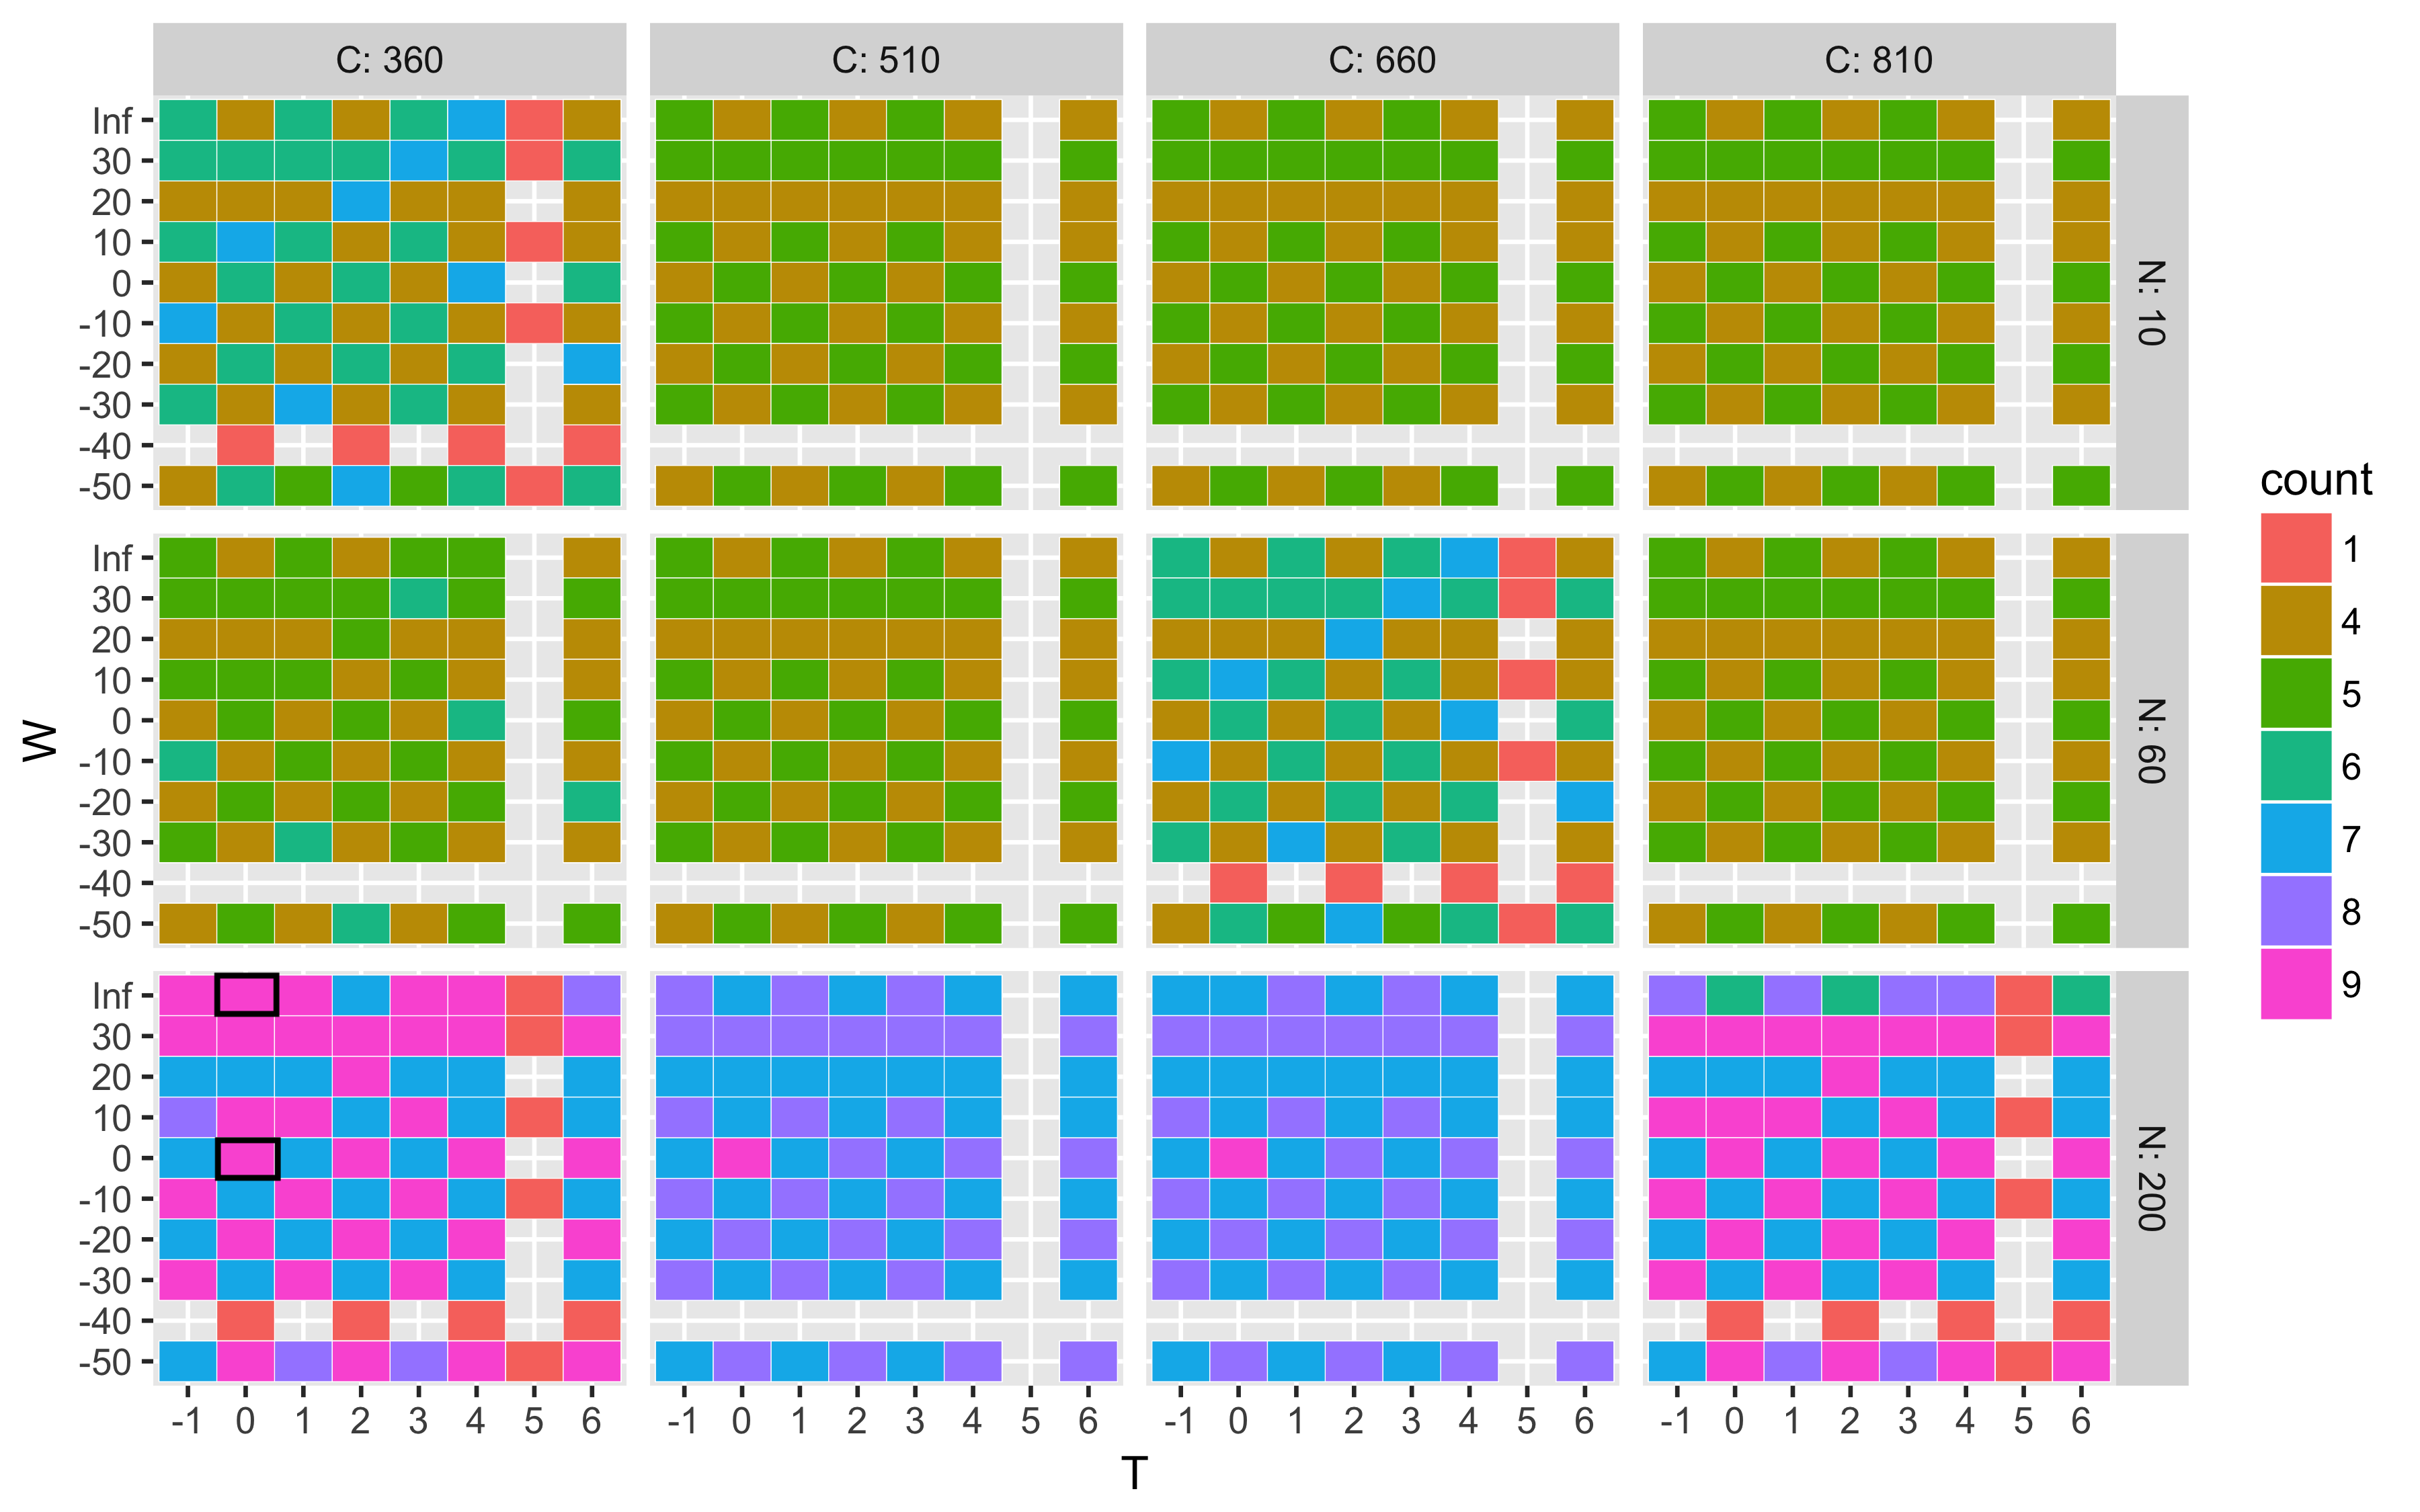
\includegraphics[width=\textwidth]{s_how_many_simulations.png}
  \caption{
  Heatmap illustrates number of model simulations provided for each of the scenarios in the variable space. 
  The max number is 9, the number of models included in the emulator analysis (excluding three models not included in the emulator analysis). 
  Normalized error calculations are run over scenarios with max number of models.
  }
  \label{fig:numbersims}
\end{figure}

\clearpage
\section{Cultivation areas}
\begin{figure}[h!]
\centering
\begin{minipage}{.45\textwidth}
    \centering
    \vspace{0pt}
    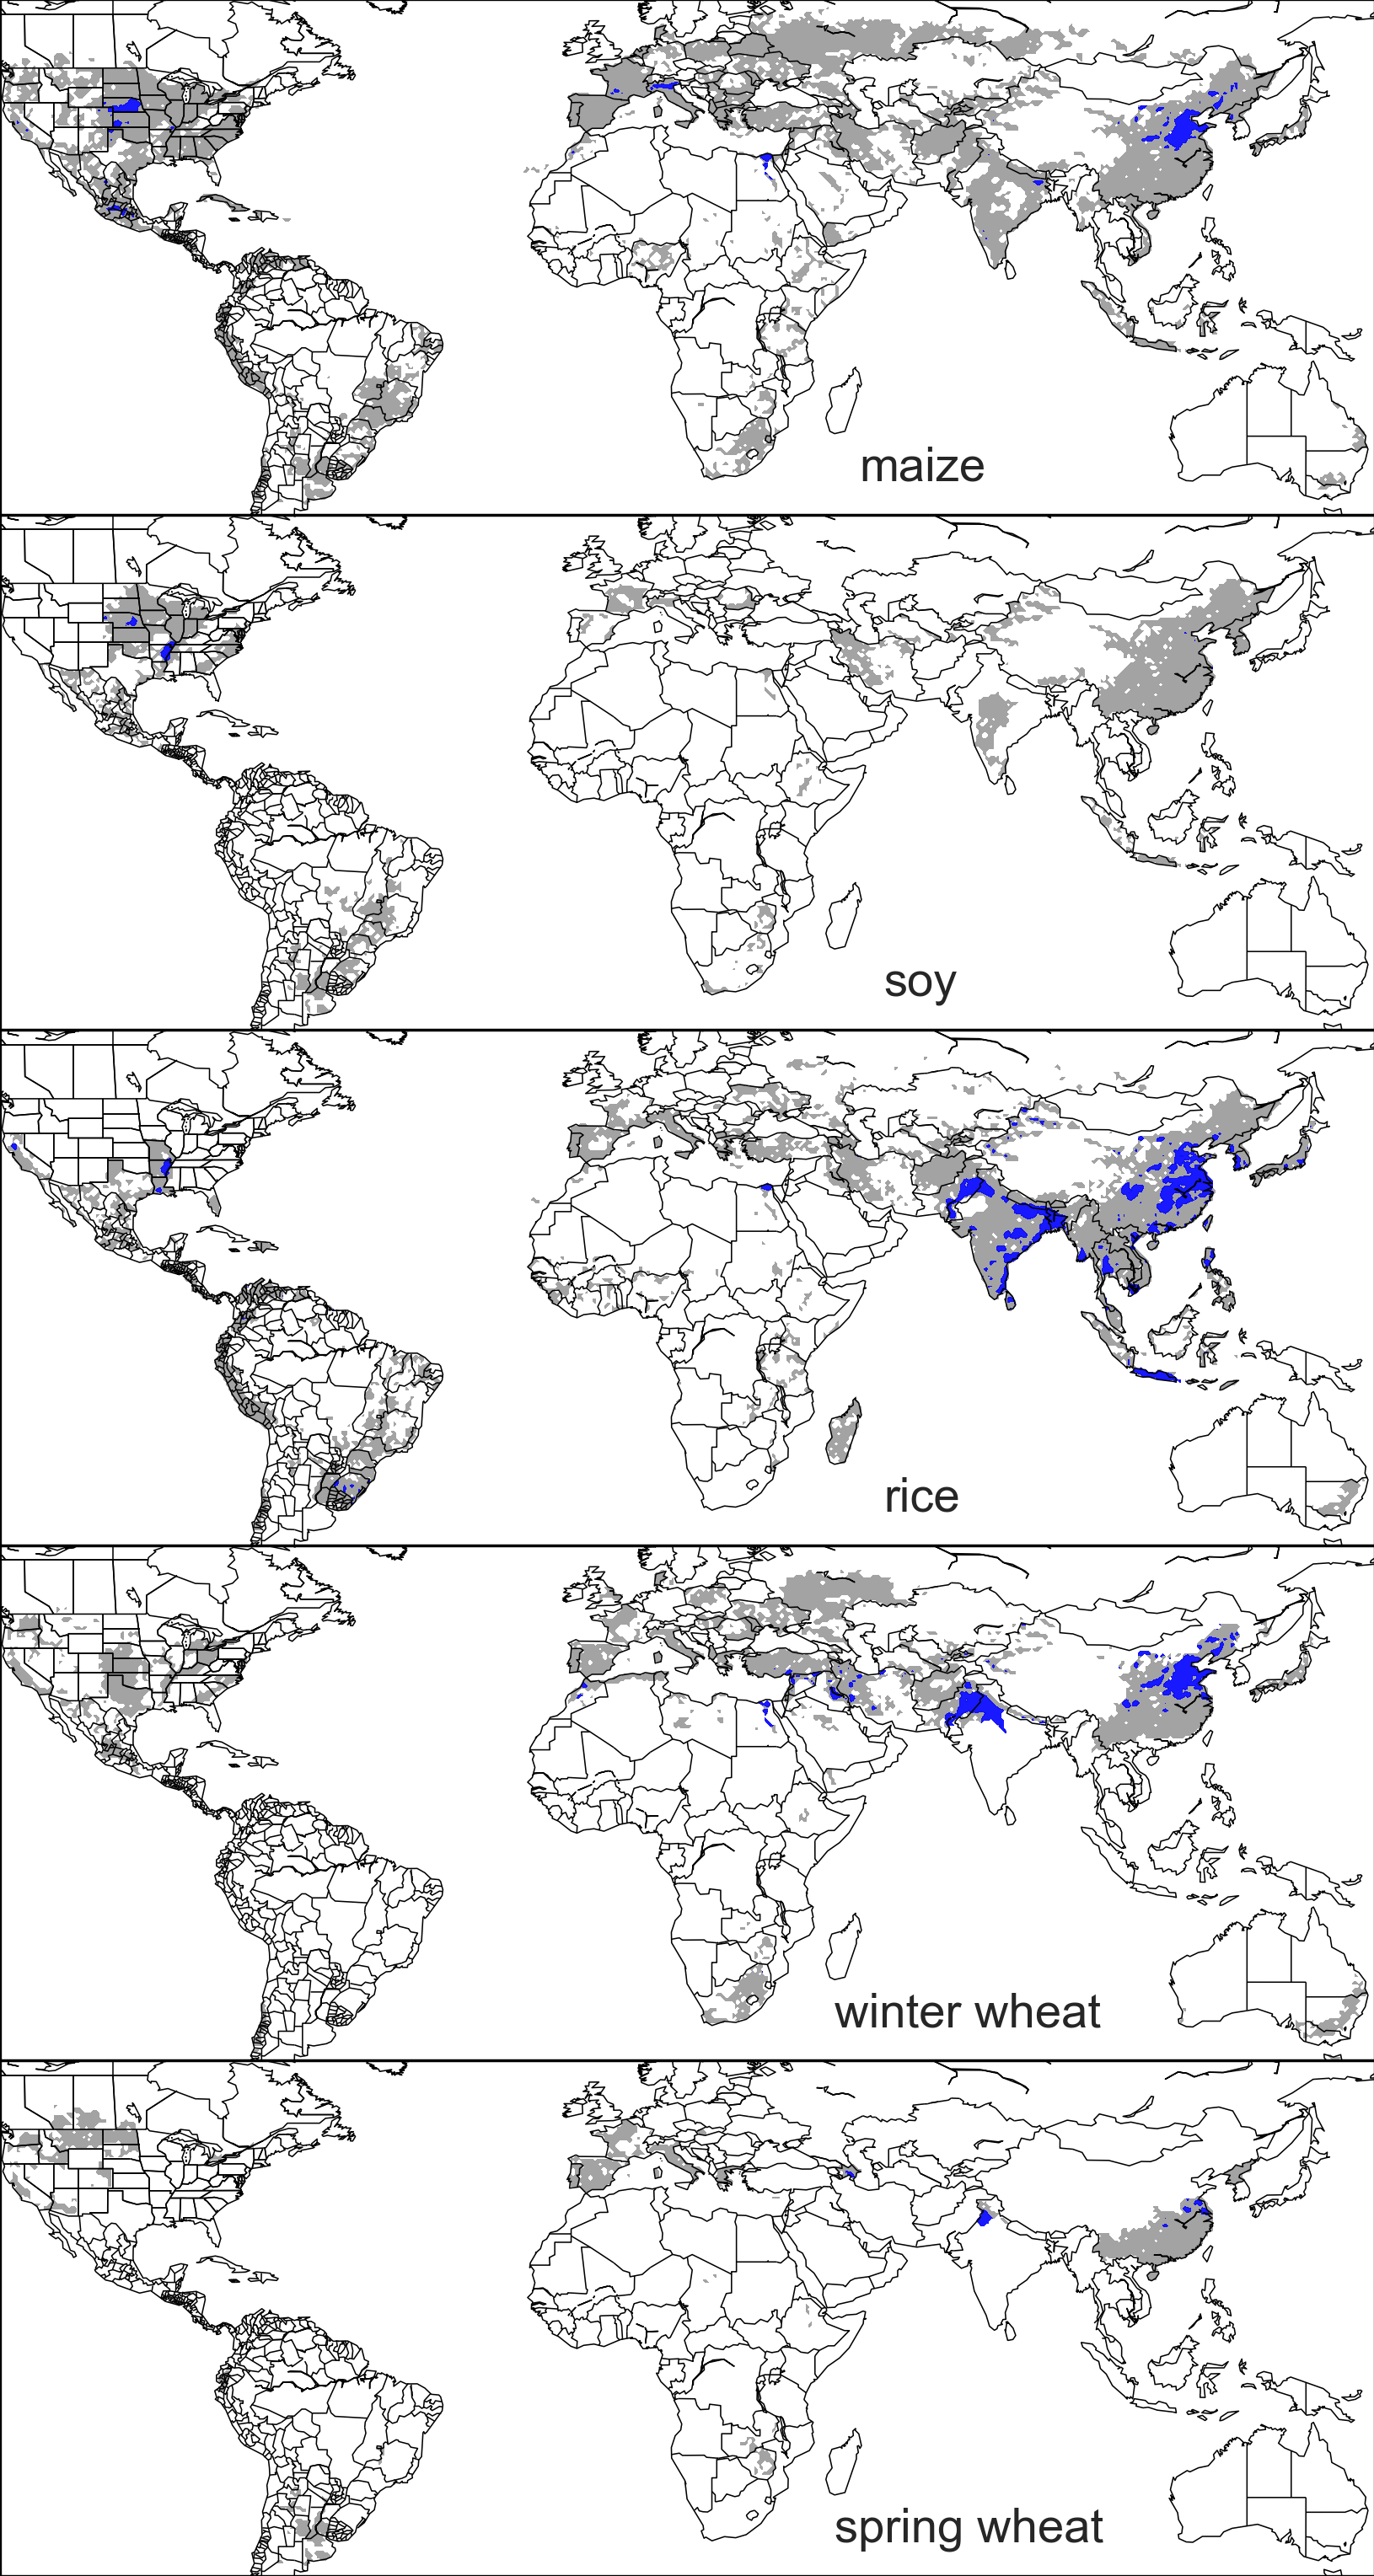
\includegraphics[width=\textwidth]{s_croparea_irr.png}\\
    \caption{
    Presently cultivated area for irrigated crops in the real world. 
    The blue contour area indicates grid-cells with more that 20,00 hectares of crop cultivated. 
    The gray contour shows area with more that 10 hectares cultivated. Data from the MIRCA2000 data set for maize, rice, and soy. 
    Winter and spring wheat areas are adapted from MIRCA2000 data and sorted by growing season
    }
    \label{fig:irrarea}
\end{minipage}
\hspace{.05\linewidth}
%S2
\begin{minipage}{.45\textwidth}
    \centering
    \vspace{-19mm}
    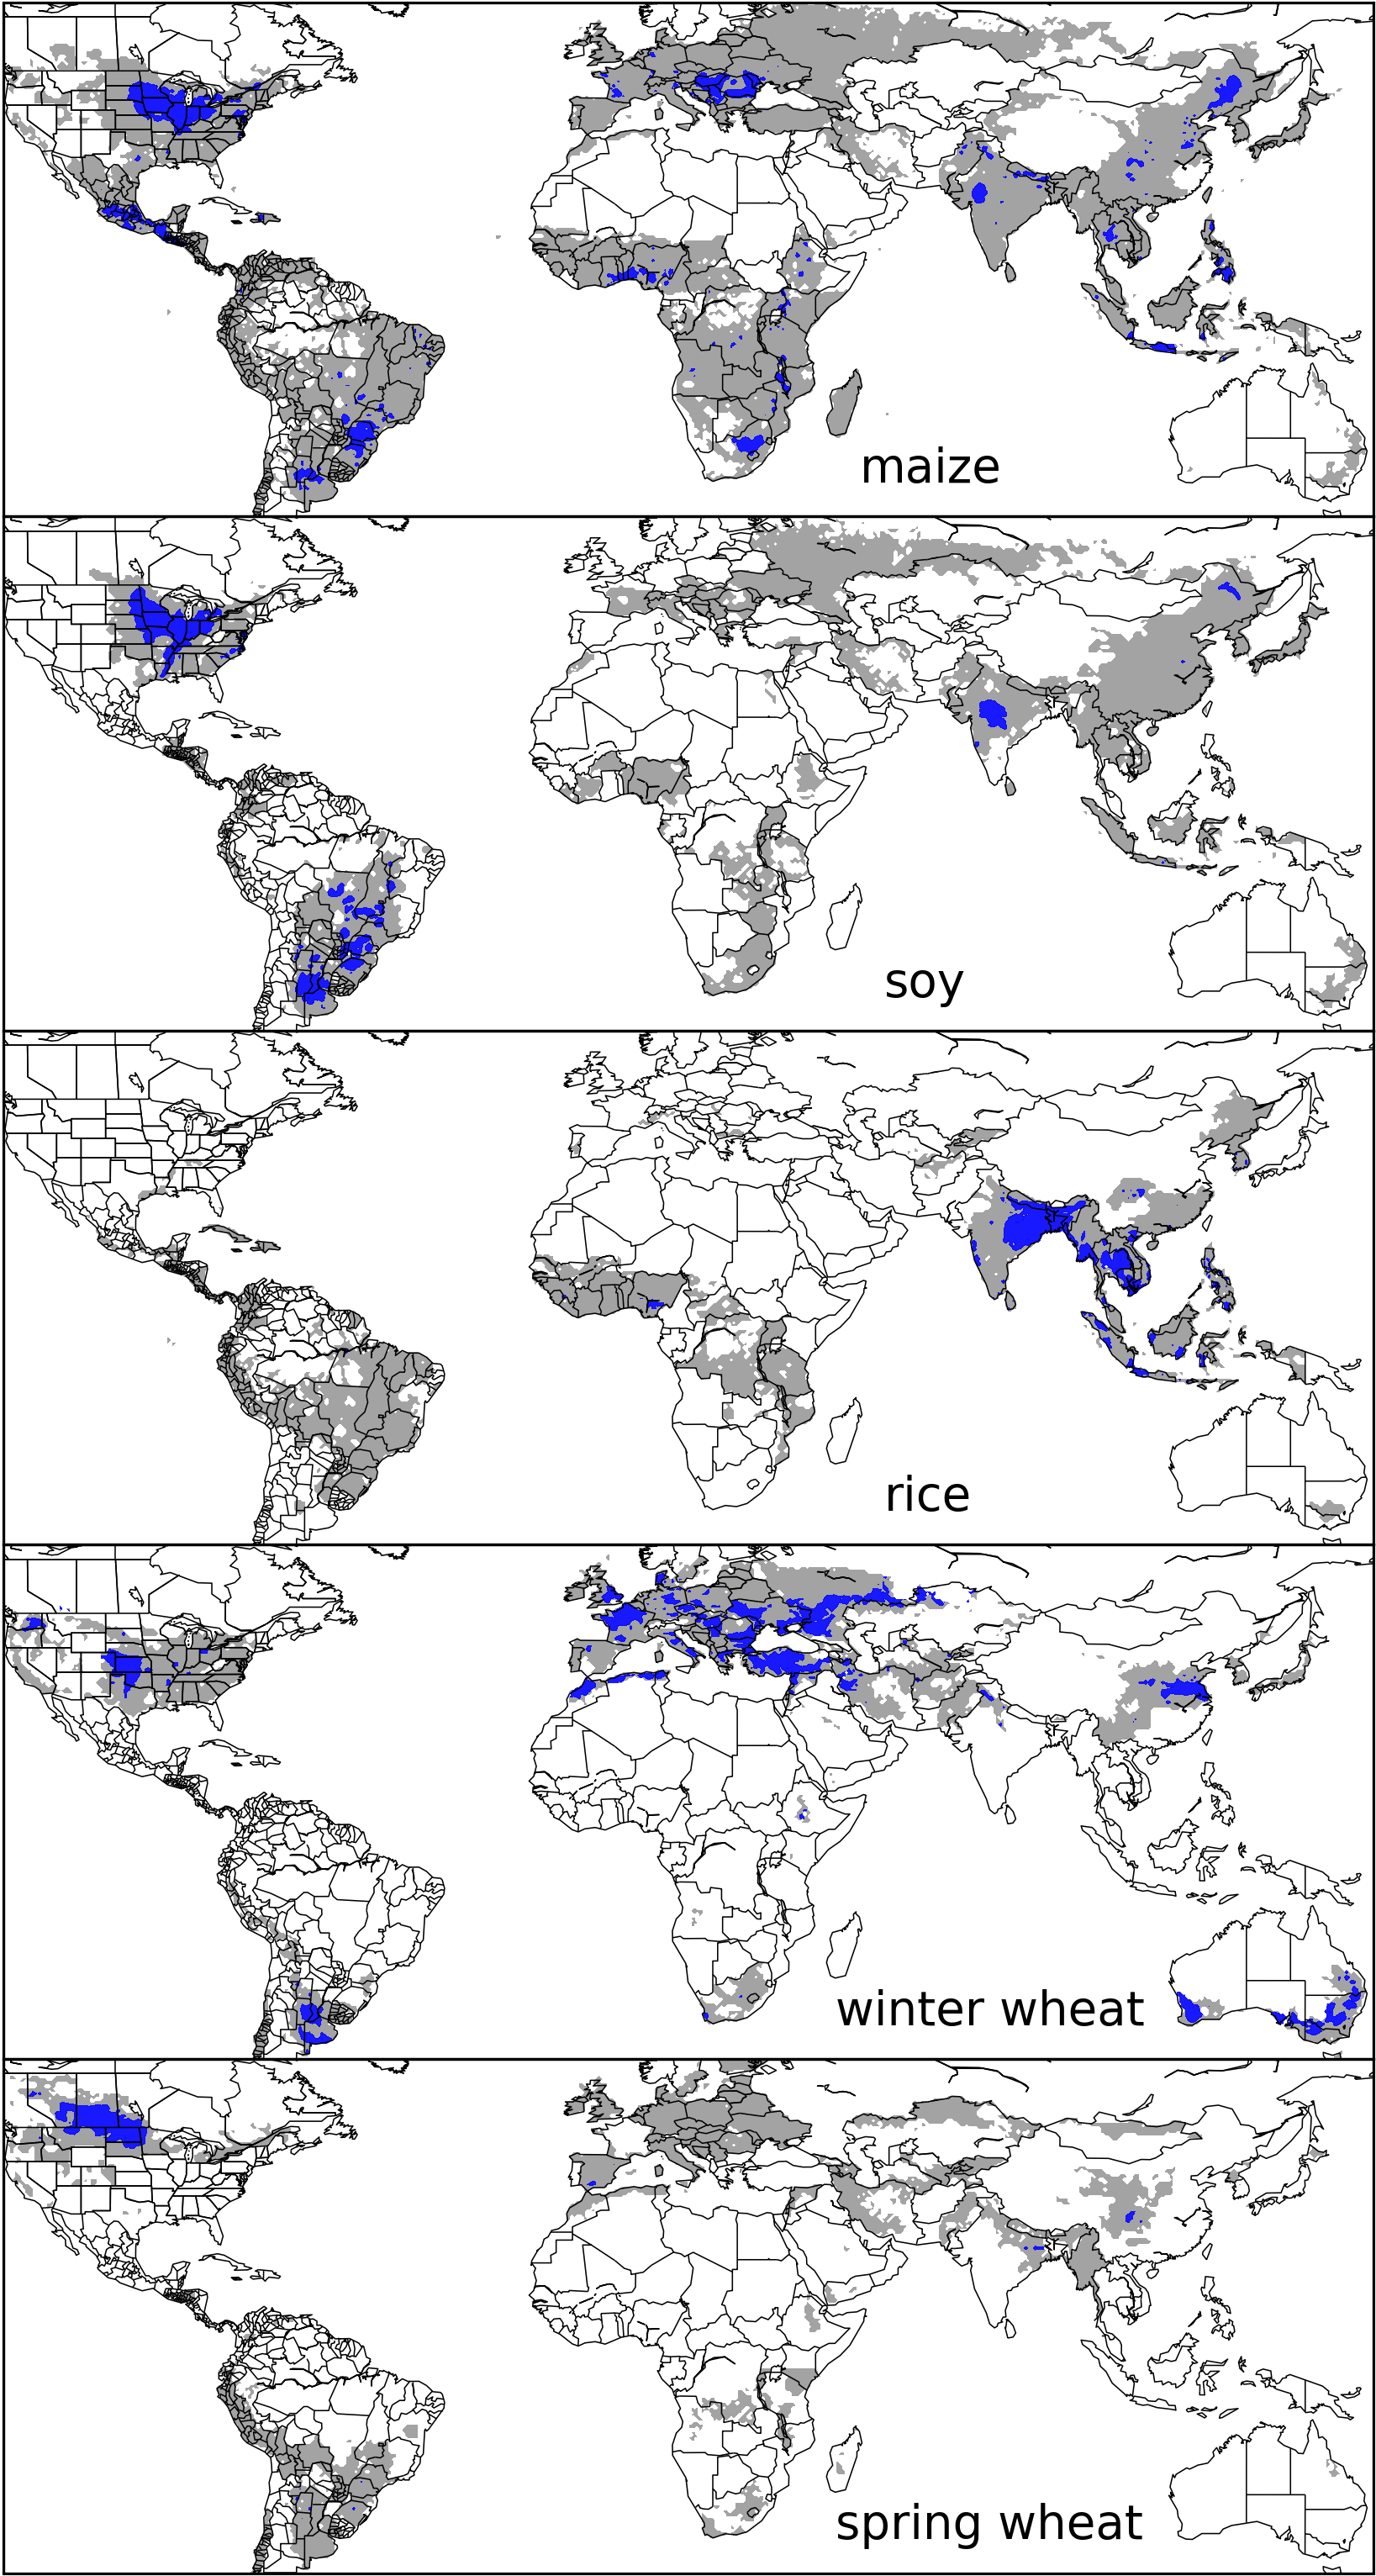
\includegraphics[width=\textwidth]{s_croparea.png}\\
    \caption{Presently cultivated area for rain fed crops in the real world. Conventions as in Figure S1.}
    \label{fig:rainfed}
\end{minipage}
\end{figure}

%%%%%%%%%%%%%%%%%%%%%%%%%%%%%%%%%%%%%%%%%%%%%%%%%%%%%%%%%%%%%%%%%%%%%%%%%%%%%%%%%%%%%%%
%%%%%%%%%%%%%%%%%%%%%%%%%%%%%%%%%%%%%%%%%%%%%%%%%%%%%%%%%%%%%%%%%%%%%%%%%%%%%%%%%%%%%%%
%%%%%%%%%%%%%%%%%%%%%%%%%%%%%%%%%%%%%%%%%%%%%%%%%%%%%%%%%%%%%%%%%%%%%%%%%%%%%%%%%%%%%%%
\clearpage
\section{Yield response for A1 simulations}
\begin{figure}[h!]
\centering
    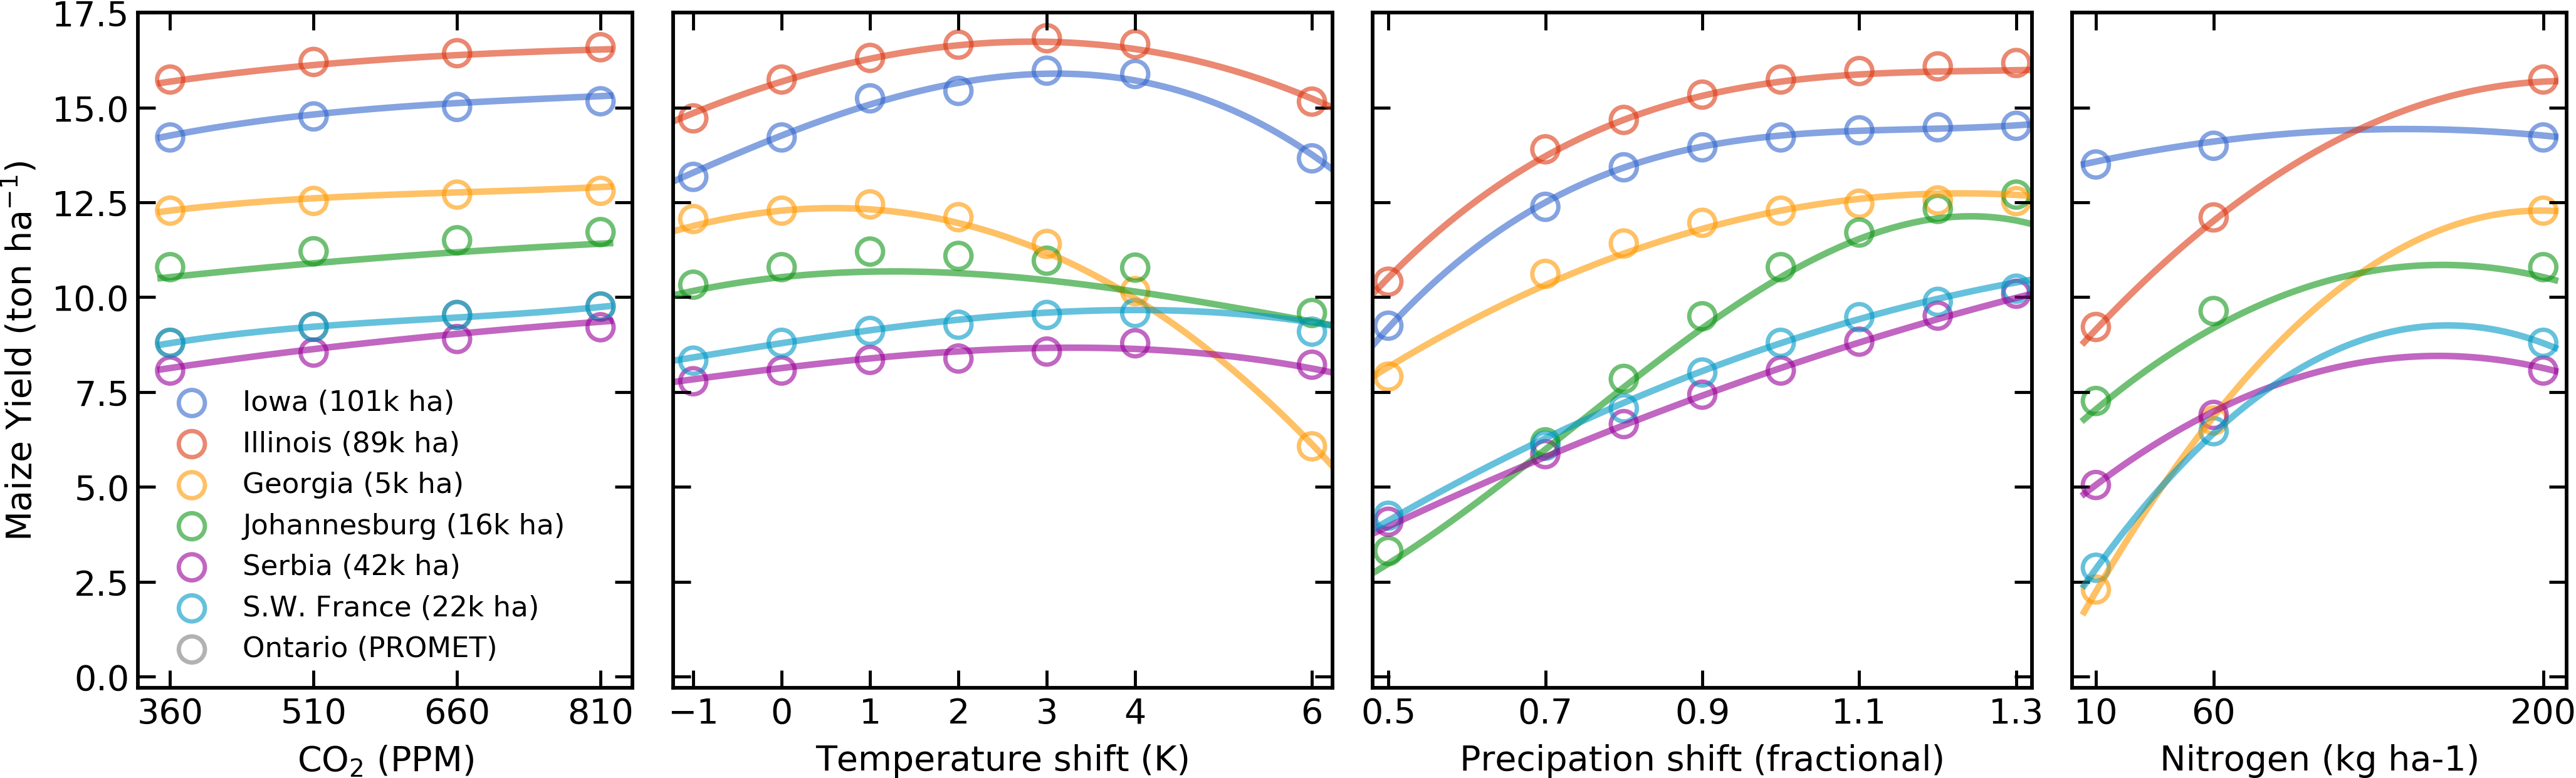
\includegraphics[width=16.3cm]{regression_exampleA1.png}
    \caption{
    Illustration of spatial variations in yield response, which are successfully captured by the emulator for the A1 simulations. 
    Panels show simulations (points) and emulations (lines) of rainfed maize in the pDSSAT model in six example locations selected to represent high-cultivation areas around the globe. 
    Legend includes hectares cultivated in each selected grid cell. 
    Each panel shows variation along a single variable, with others held at baseline values. 
    }
   \label{fig:regression}
\end{figure}

\begin{figure}[h!]
\centering
    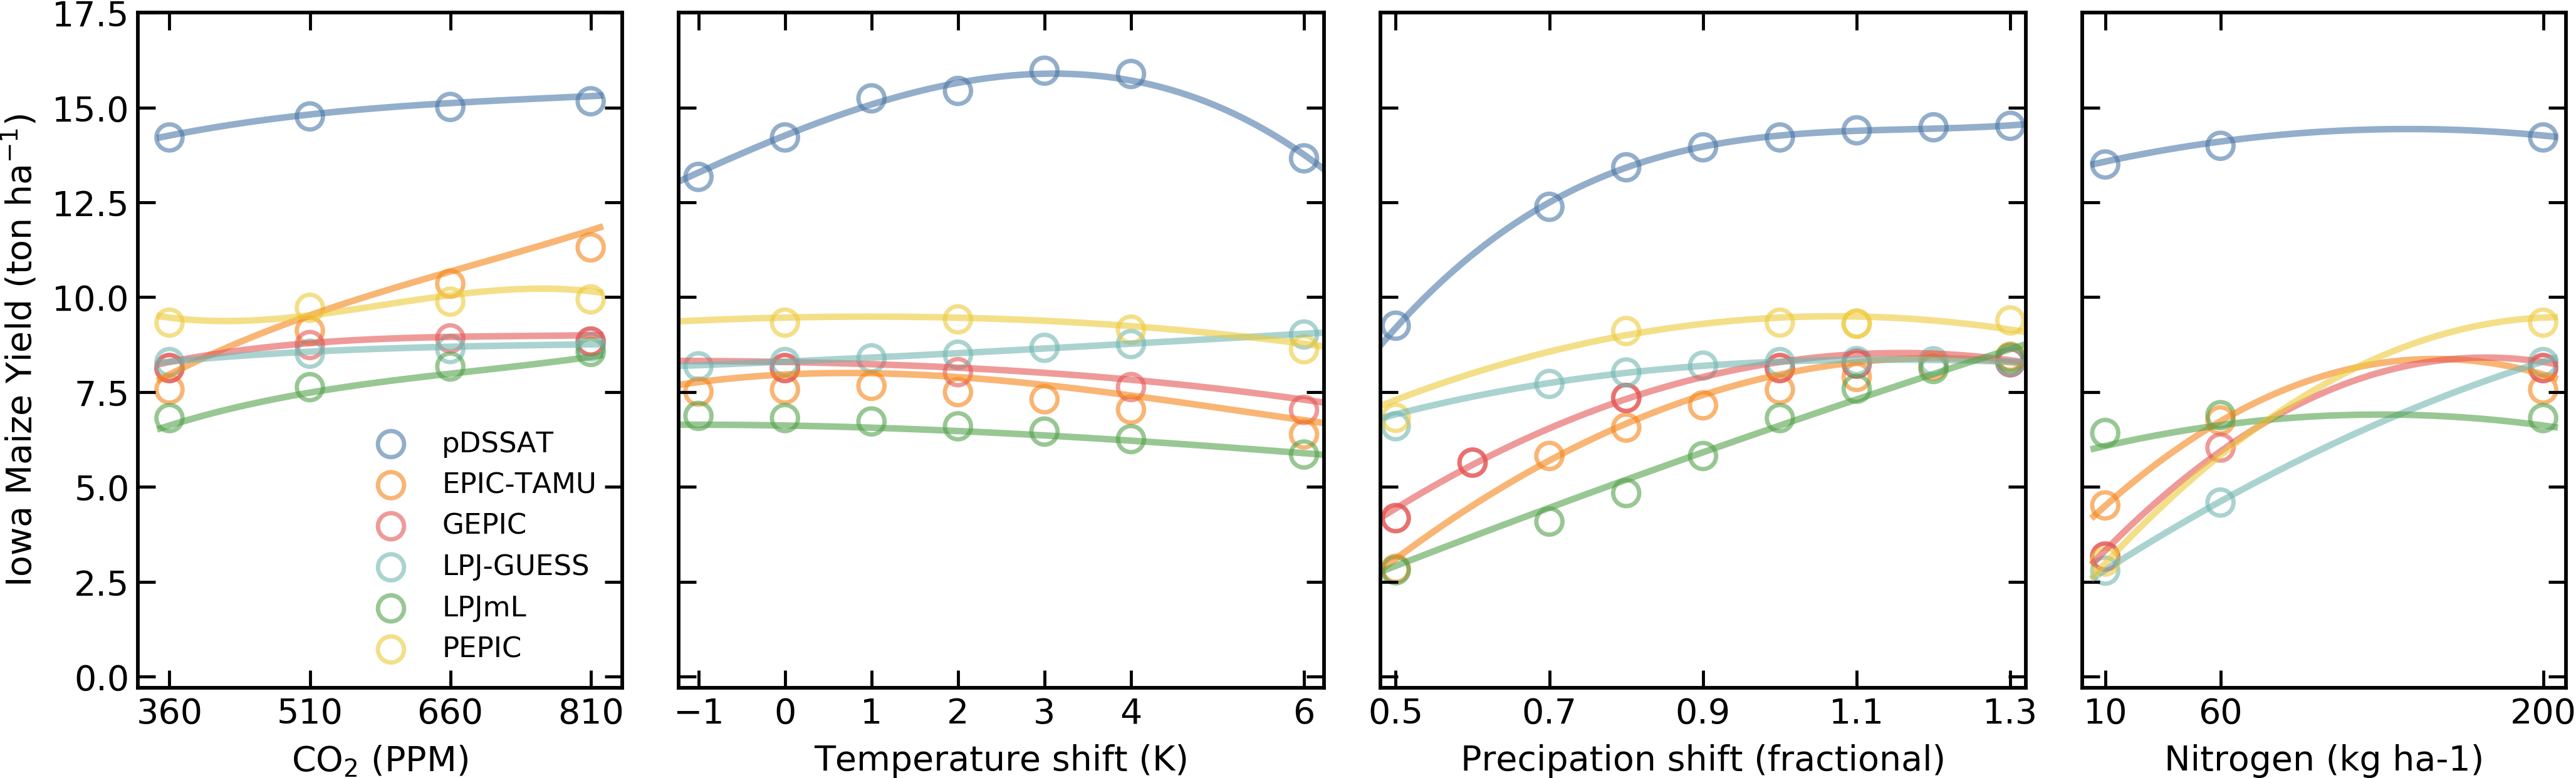
\includegraphics[width=16.3cm]{regression_exampleA1_2.png}
    \caption{
    Illustration of variations in yield response across models, again successfully captured by the emulator. 
    Panels show simulations and emulations from six representative GGCMI models for rainfed maize in the same Iowa grid cell shown above, with the same plot conventions. 
    Three models (PROMET, JULES, and CARAIB) that do not simulate the nitrogen dimension are omitted for clarity. 
    Models are uncalibrated, producing spread in absolute yields. 
    }
   \label{fig:regression_2}
\end{figure}

%%%%%%%%%%%%%%%%%%%%%%%%%%%%%%%%%%%%%%%%%%%%%%%%%%%%%%%%%%%%%%%%%%%%%%%%%%%%%%%%%%%%%%%
%%%%%%%%%%%%%%%%%%%%%%%%%%%%%%%%%%%%%%%%%%%%%%%%%%%%%%%%%%%%%%%%%%%%%%%%%%%%%%%%%%%%%%%
%%%%%%%%%%%%%%%%%%%%%%%%%%%%%%%%%%%%%%%%%%%%%%%%%%%%%%%%%%%%%%%%%%%%%%%%%%%%%%%%%%%%%%%

\clearpage
\section{Normalized error for other cases}

\begin{figure}[h!]
  \centering
  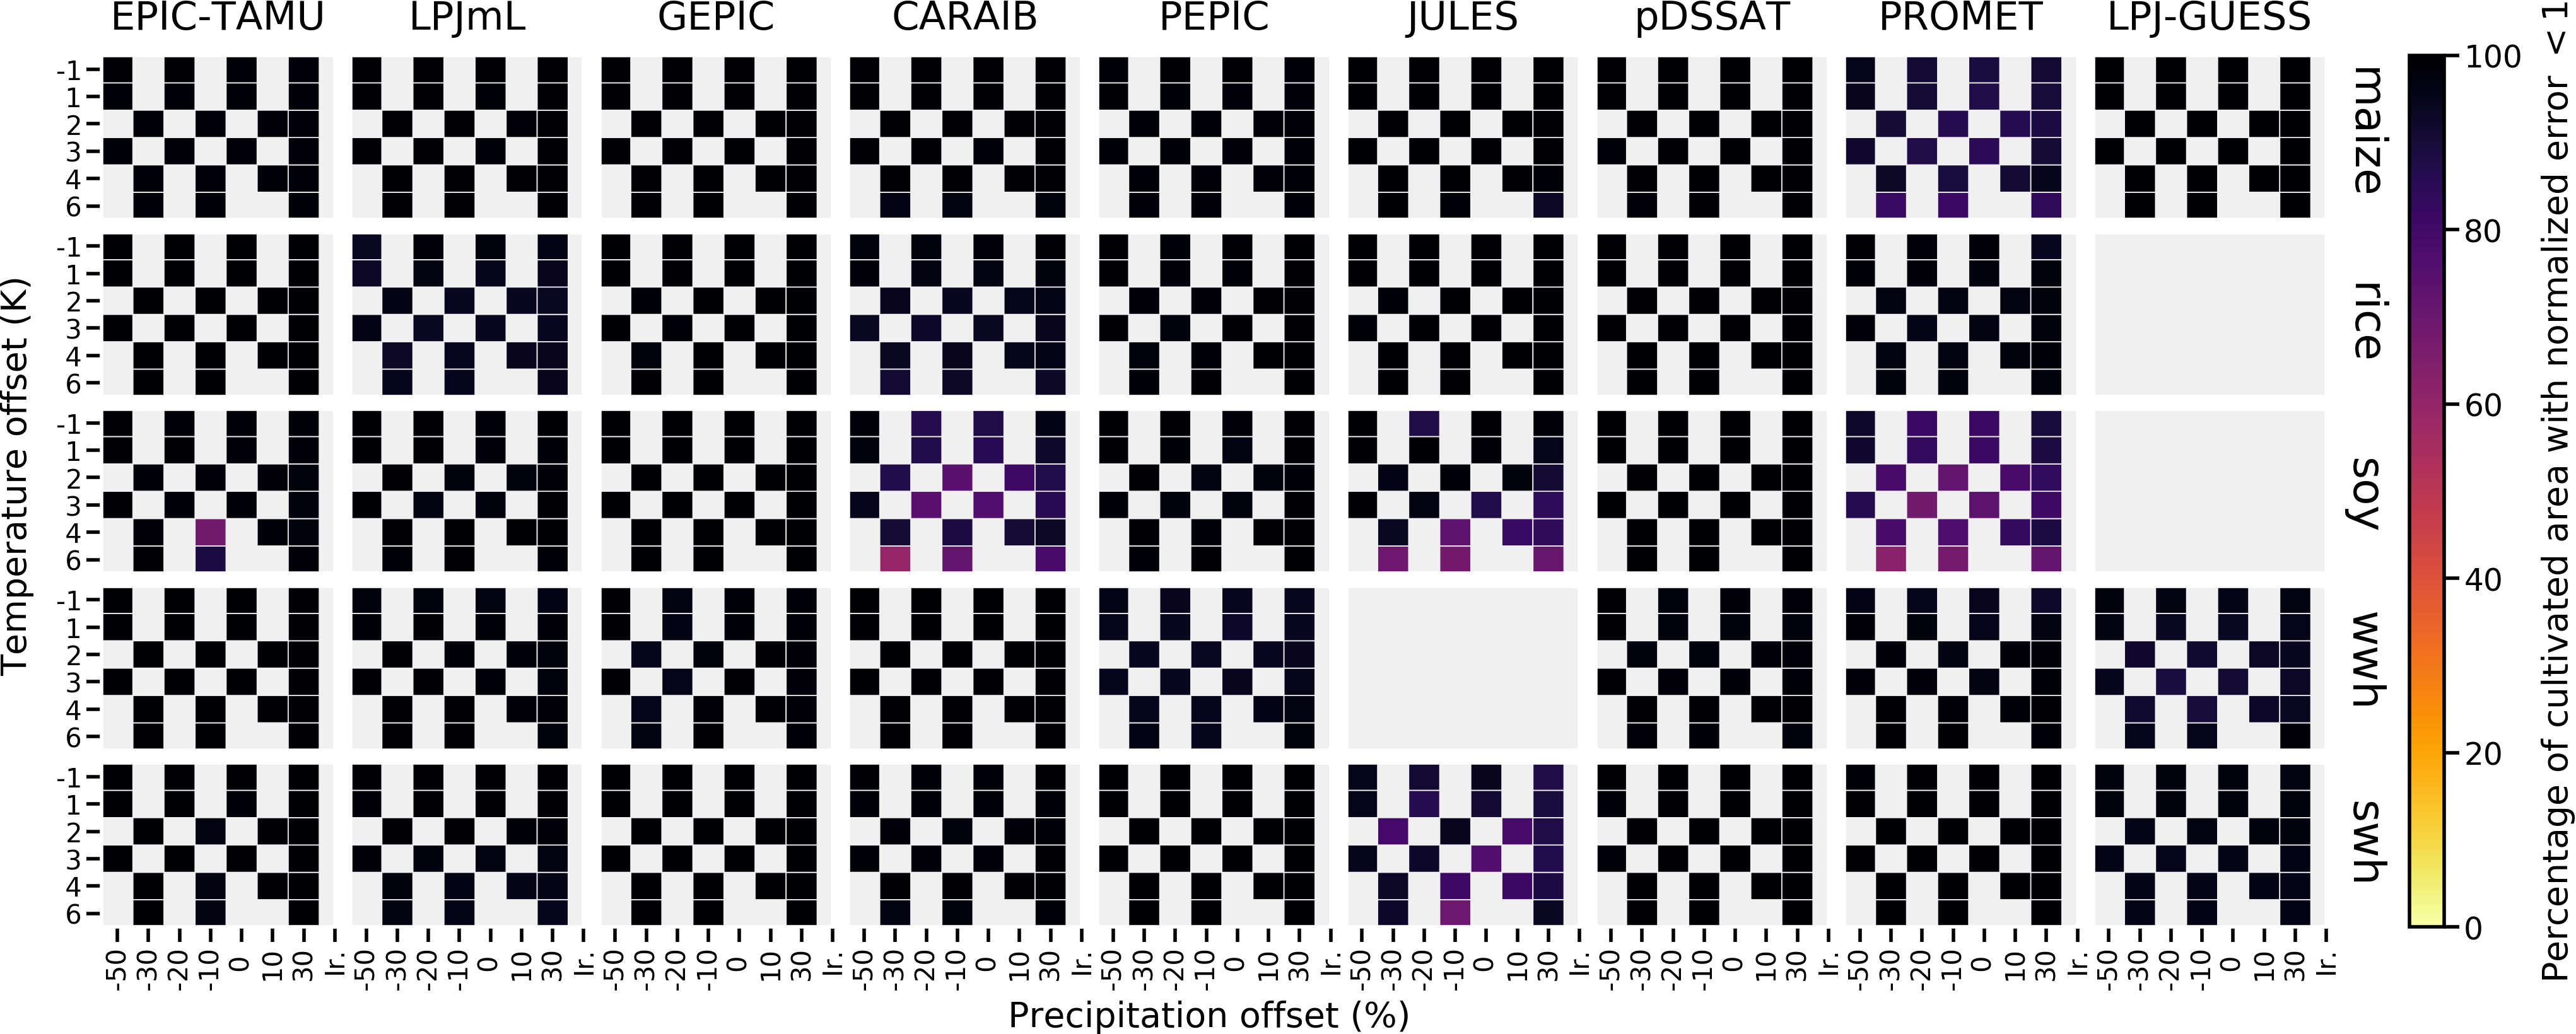
\includegraphics[width=15.5cm]{error_grid_810.png}
  \caption{
  The fraction of currently cultivated hectares with normalized emulation error less than 1 for the CO$_2$=810 ppm and 200 kg~N ha$^{-1}$ yr$^{-1}$ case for the temperature and precipitation perturbations scenarios provided by all 9 models included in the emulator analysis. 
  The yield response is generally easy to emulate over currently cultivated areas (black regions).
  }
  \label{fig:error810}
\end{figure}

\begin{figure}[h!]
  \centering
  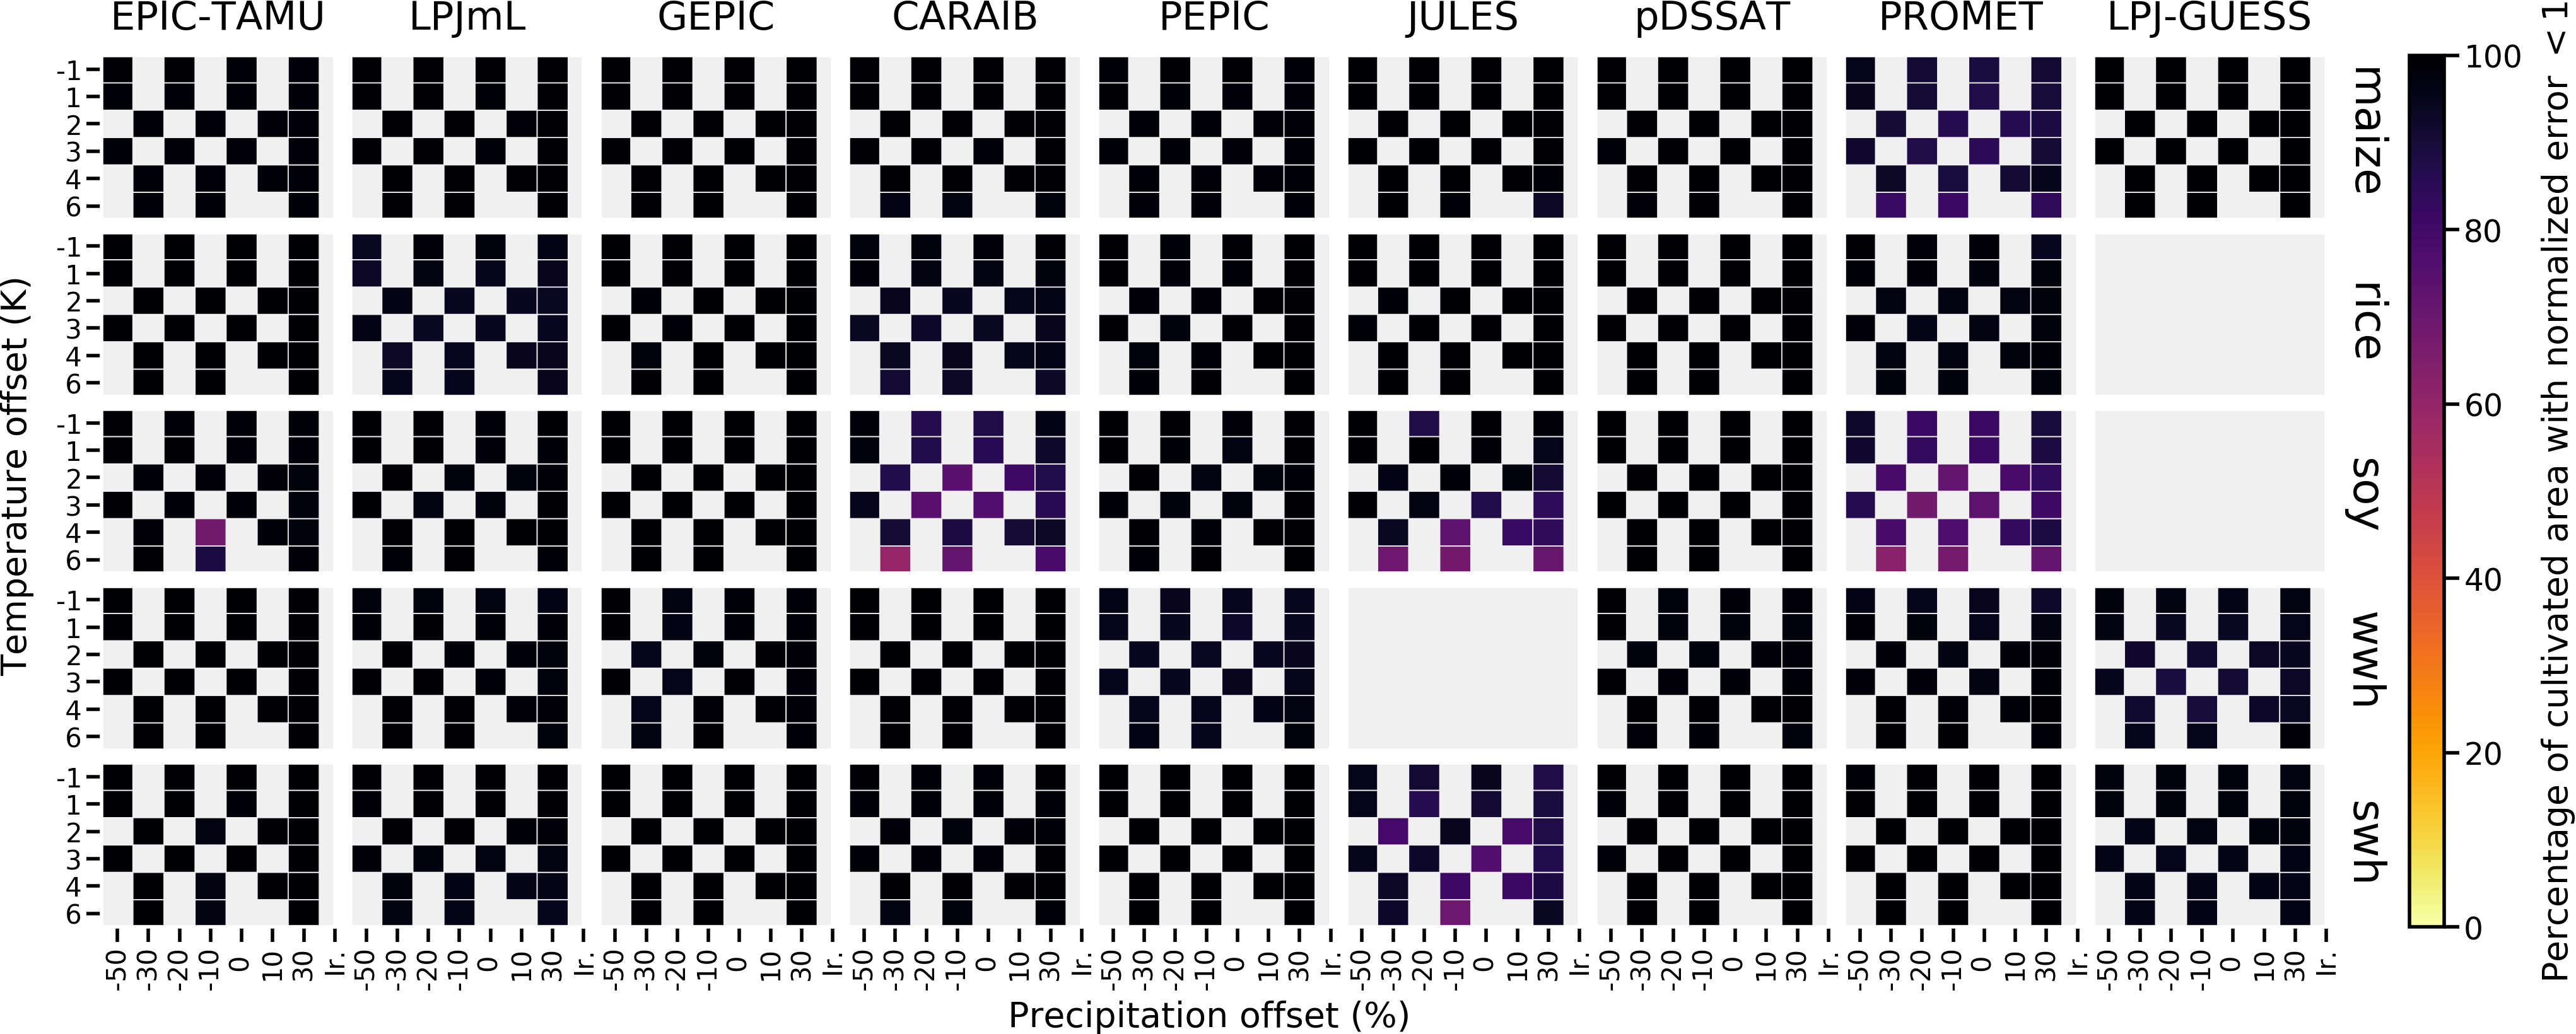
\includegraphics[width=15.5cm]{error_grid_810.png}
  \caption{
  The fraction of currently cultivated hectares with normalized emulation error less than 1 for A1 (growing season adaptation) simulations for CO$_2$=360 ppm and 200 kg~N ha$^{-1}$ yr$^{-1}$ case for the temperature and precipitation perturbations scenarios provided by all 9 models included in the emulator analysis. 
  The yield response is generally easy to emulate over currently cultivated areas (black regions).
  }
  \label{fig:error810}
\end{figure}

\begin{figure}[h!]
  \centering
  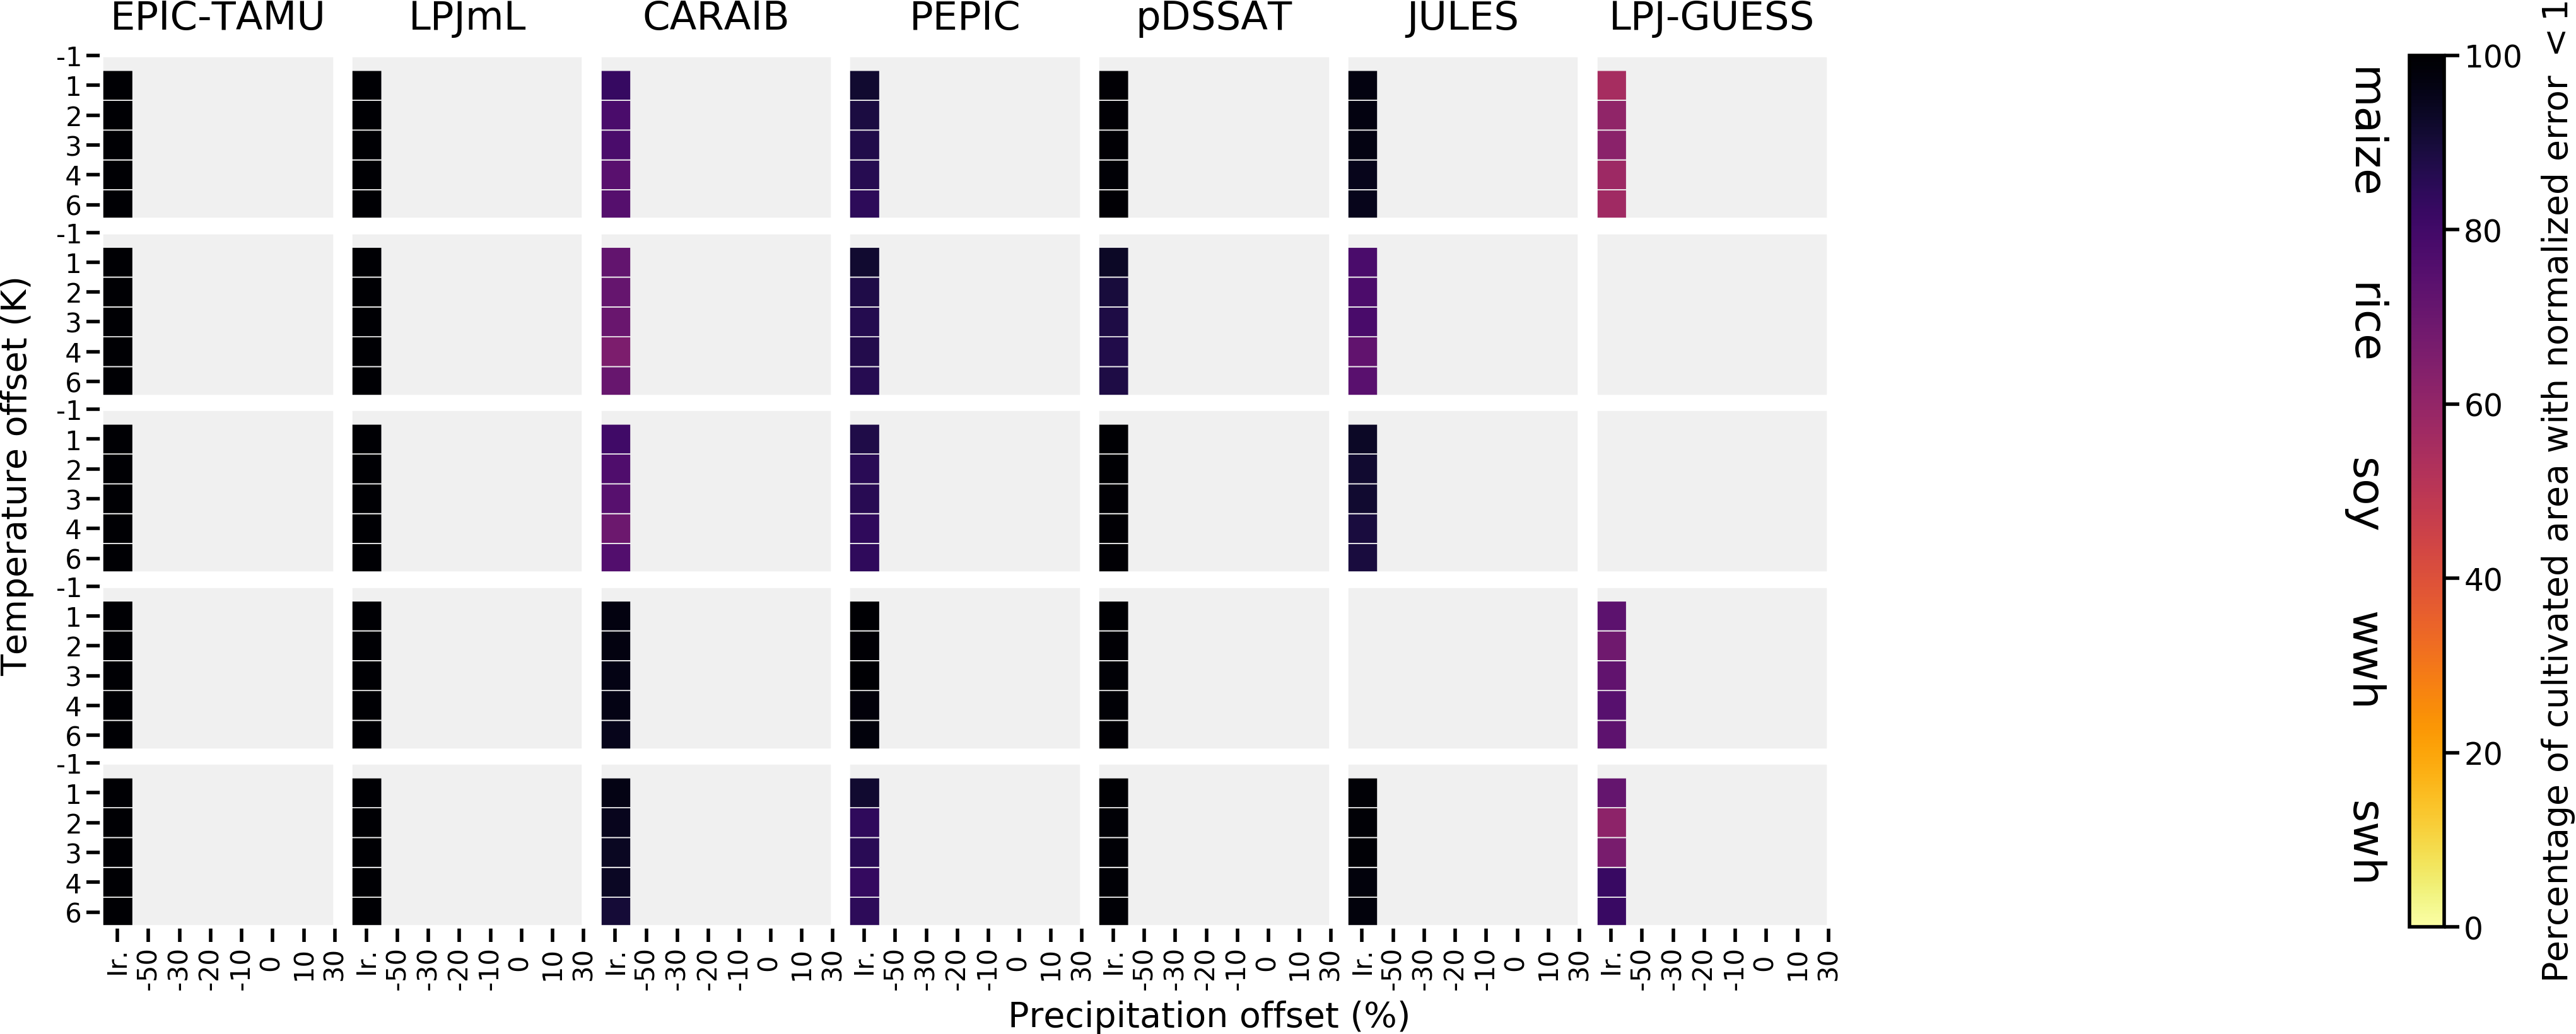
\includegraphics[width=15.5cm]{error_grid_360_cultivated_IWD.png}
  \caption{
  The fraction of currently cultivated hectares with normalized emulation error less than 1 for irrigated water demand for CO$_2$=310 ppm and 200 kg~N ha$^{-1}$ yr$^{-1}$ case for the temperature and precipitation perturbations scenarios provided by all models included for irrigation water demand in the emulator analysis. 
  }
  \label{fig:error810}
\end{figure}

\clearpage
\section{Comparison to transient climate run simulation}
\begin{figure}[h!]
  \centering
  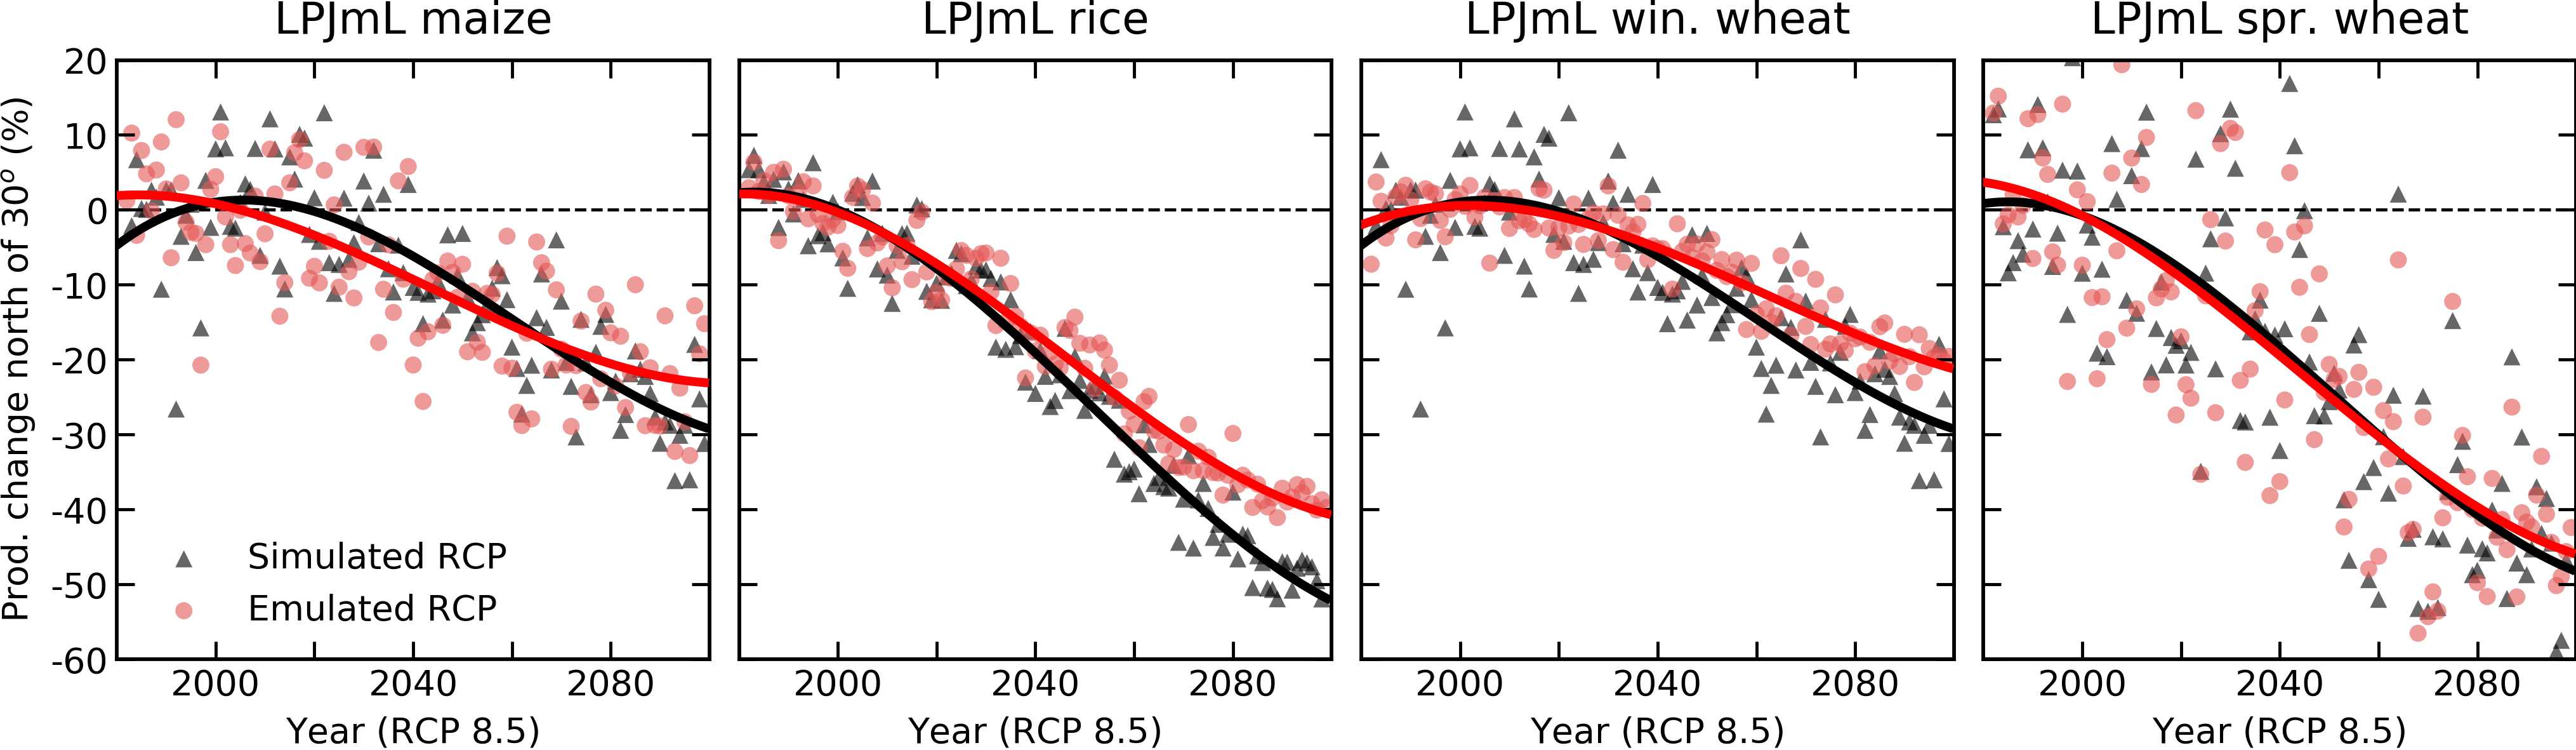
\includegraphics[width = 16.3cm]{LPJMLRCP85comp_30N.png}
  \caption{
  Same as main text Figure 9 except now only for crops north of 30N latitude.
  }
  \label{fig:lpjmlrcp}
\end{figure}

\begin{figure}[h!]
  \centering
  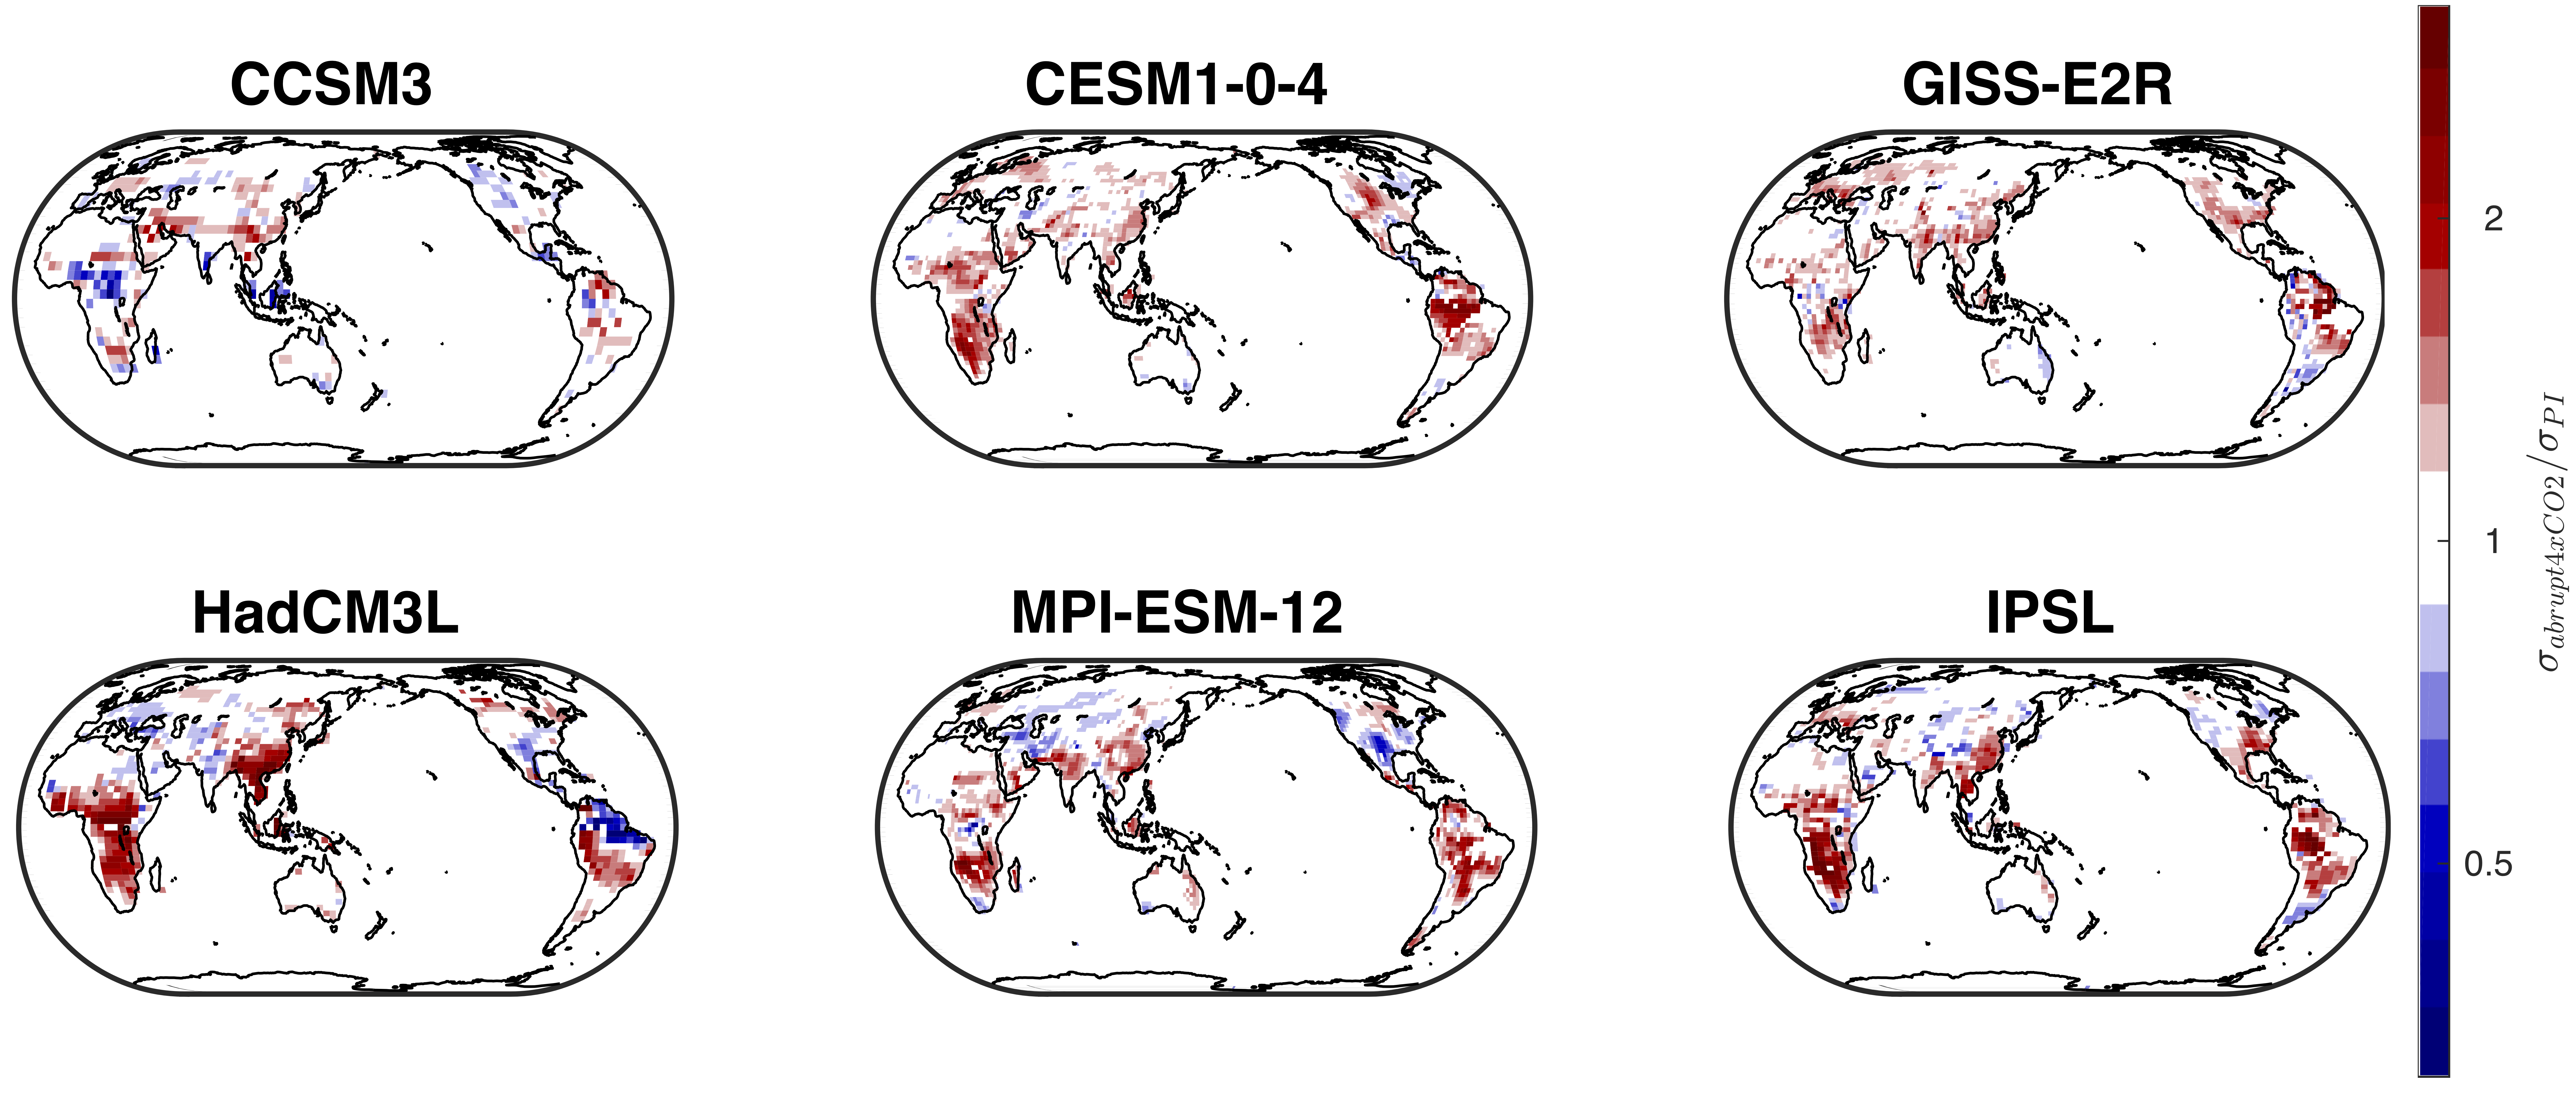
\includegraphics[width = 16.3cm]{tas_Amon_LRM6_abrupt4x_control_LF_maps_JJA_final.png}
  \caption{
  Change in hemispheric-summer variability for some CMIP-5 models for an abrupt 4x CO$_2$ forcing. Ratio in standard deviation in temperature compared to preindustrial values. 
  The HadCM3 model shows relatively strong variability changes. Model disagreement about changes in variability is large.
  }
  \label{fig:lpjmlrcp}
\end{figure}


\clearpage
\section{Emulator products}
\begin{figure}[h!]
  \centering
  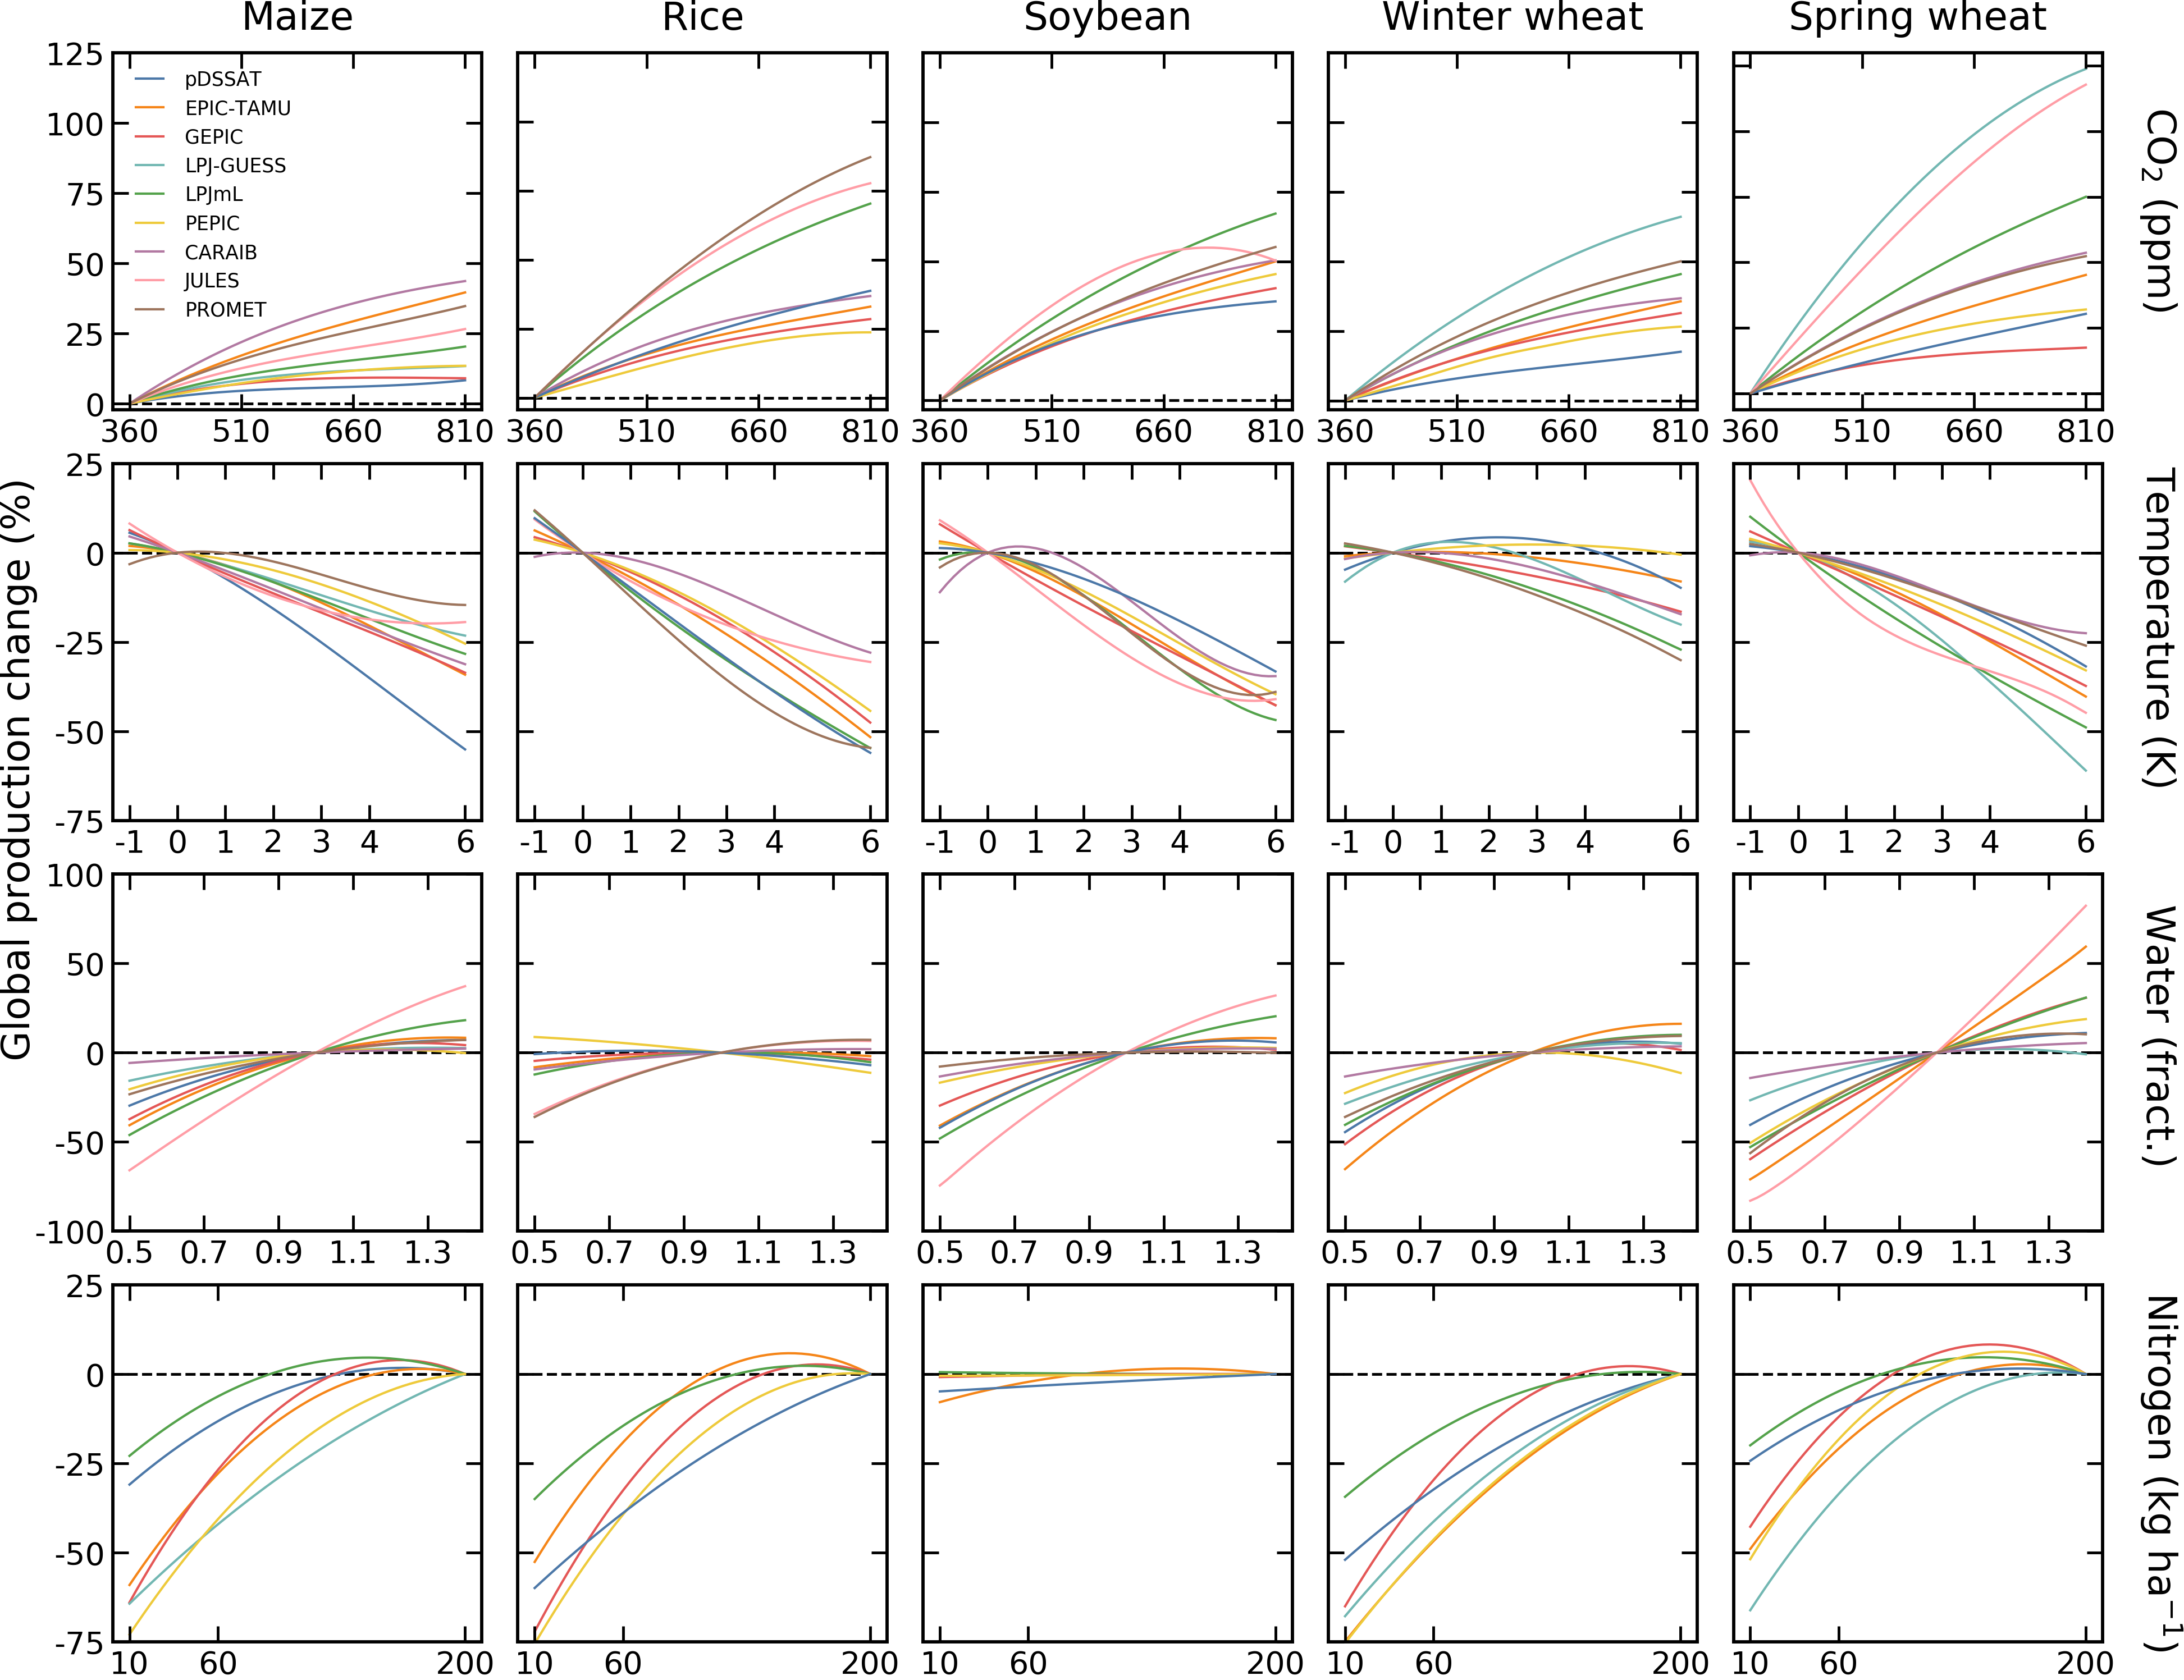
\includegraphics[width = 16.3cm]{em_CTWN_all_crops_color.png}
  \caption{
  Same as main text Figure 10 except now each model is shown in color.
  }
  \label{fig:all_dims}
\end{figure*}

\begin{figure}[h!]
  \centering
  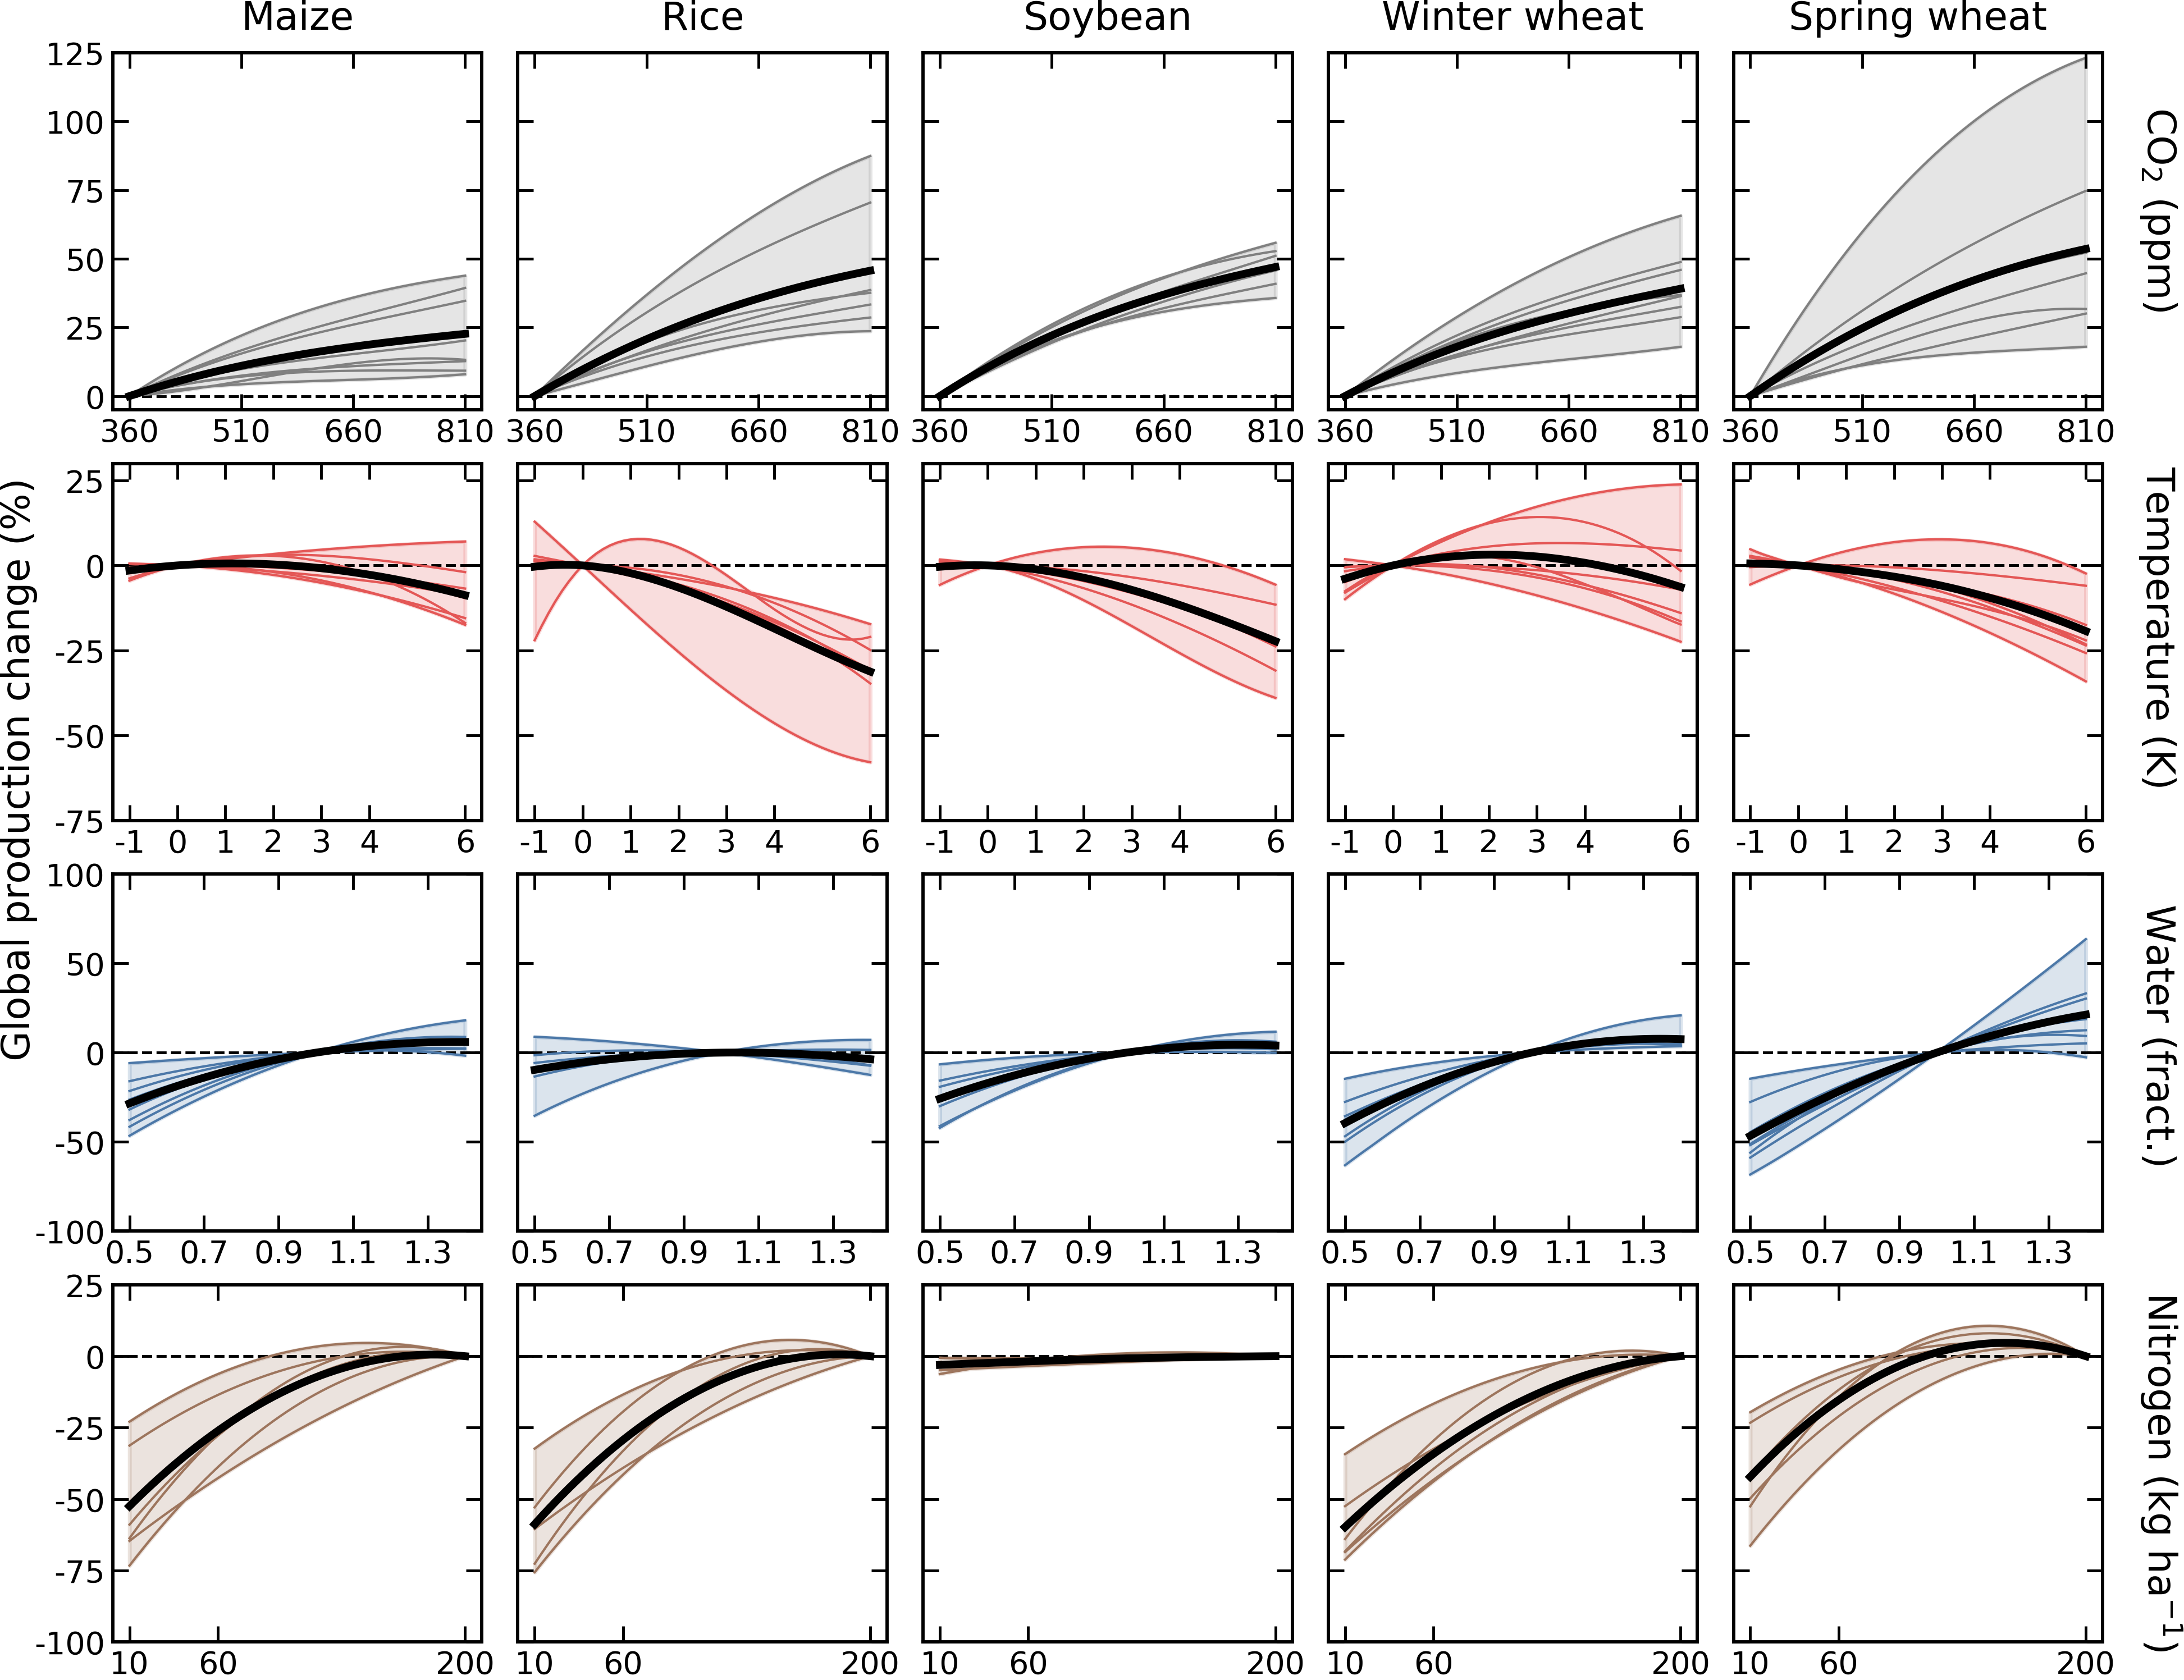
\includegraphics[width = 16.3cm]{em_CTWN_all_crops_A1.png}
  \caption{
  Emulated damage functions for rainfed crops for A1 simulations. Note: JULES does not provide A1 simulations.
  }
  \label{fig:all_dims}
\end{figure}

\begin{figure}[h!]
  \centering
  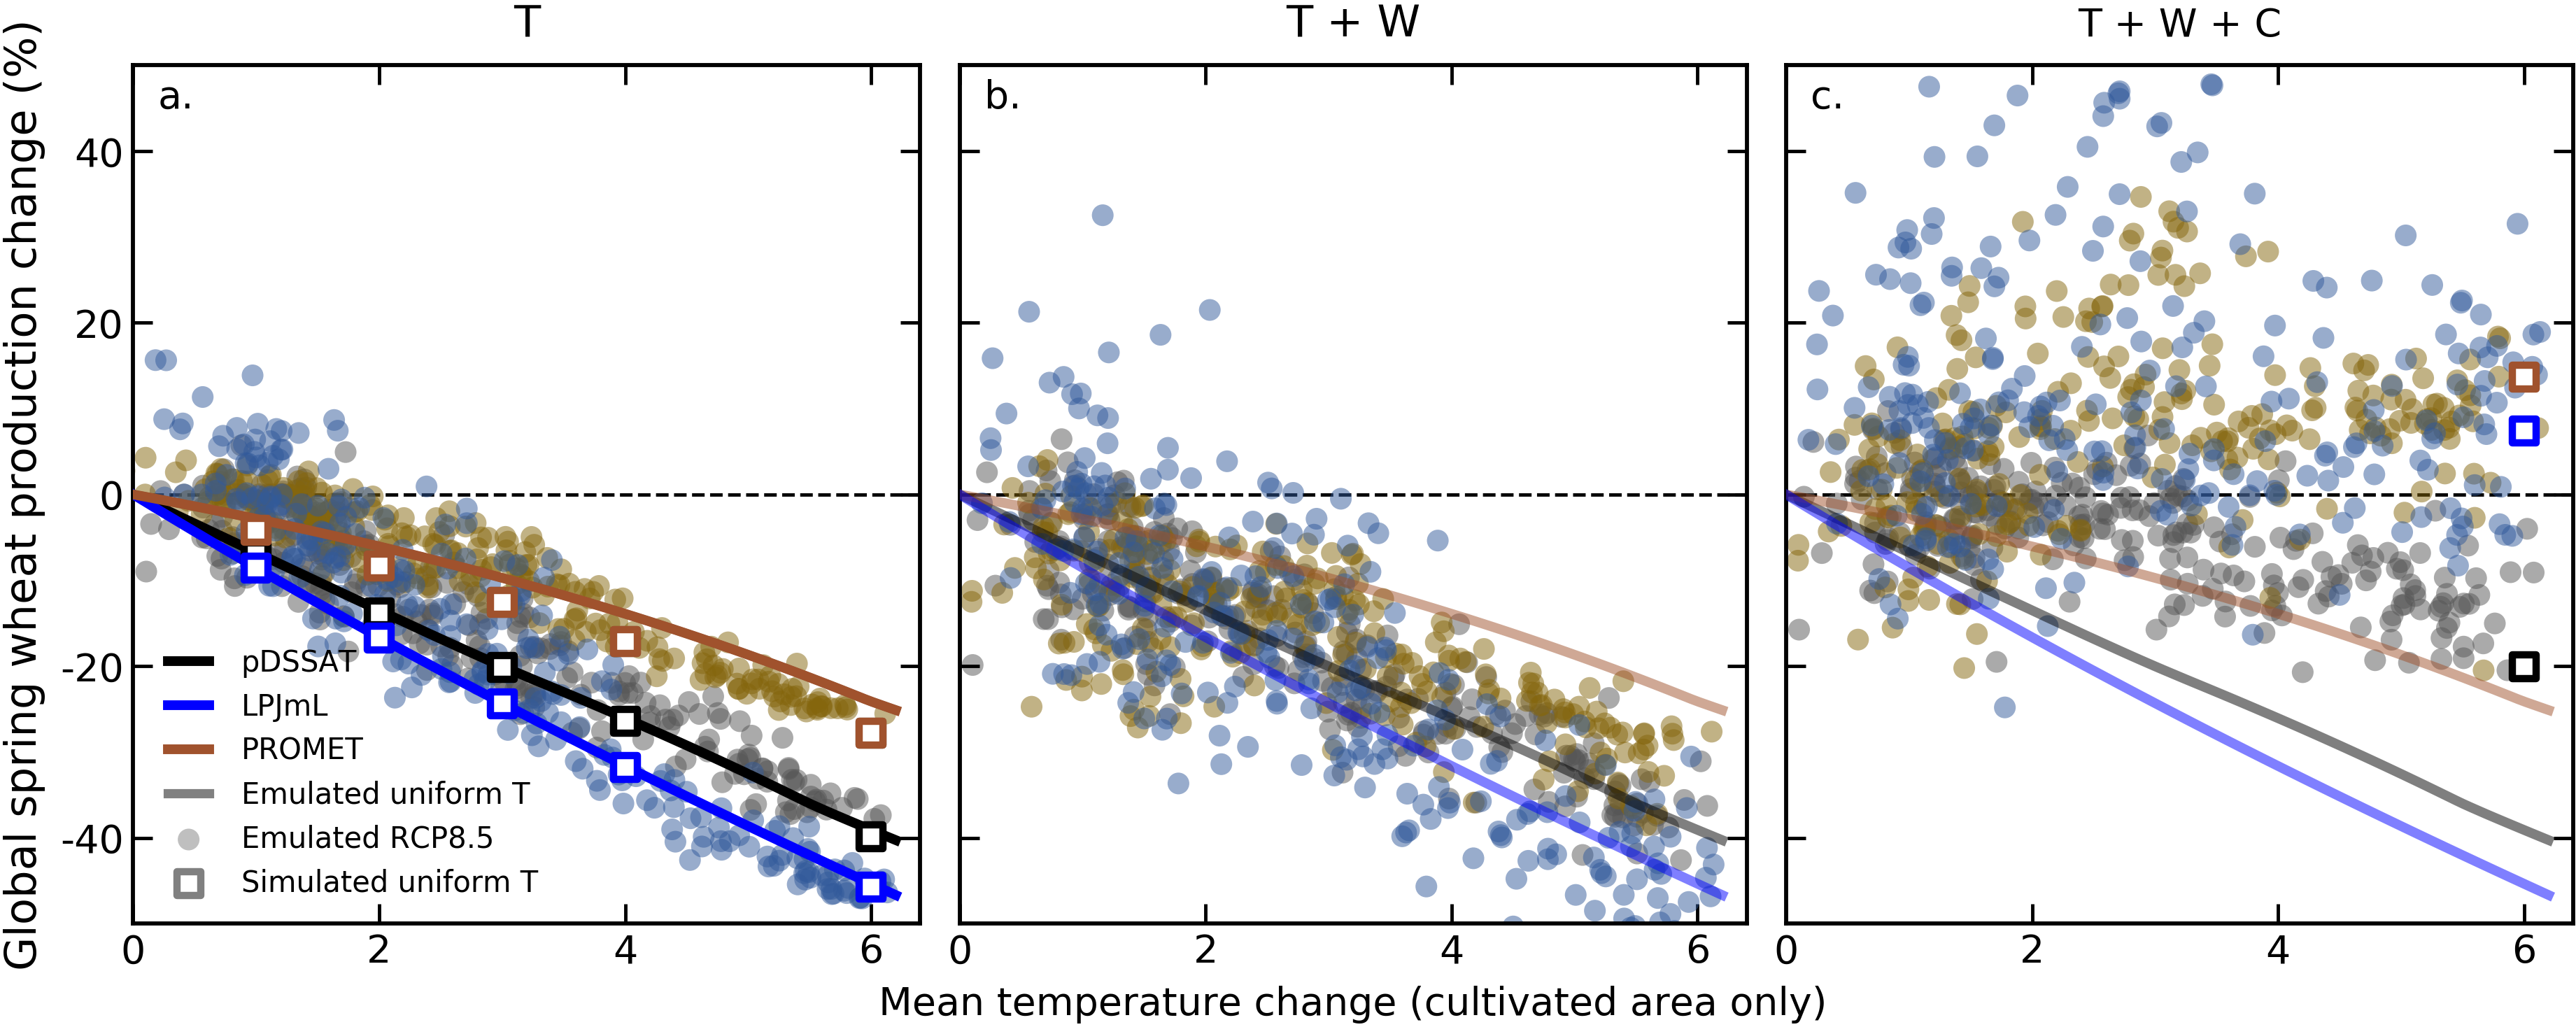
\includegraphics[width = 16.3cm]{LPJmL_pDSSAT_PROMET_RCP85_all_cases_spring_wheat.png}
  \caption{
  Illustration of the factors affecting yields in more realistic climate scenarios for spring wheat. Same convention main text Figure 11.
  }
\end{figure}

\begin{figure}[h!]
  \centering
  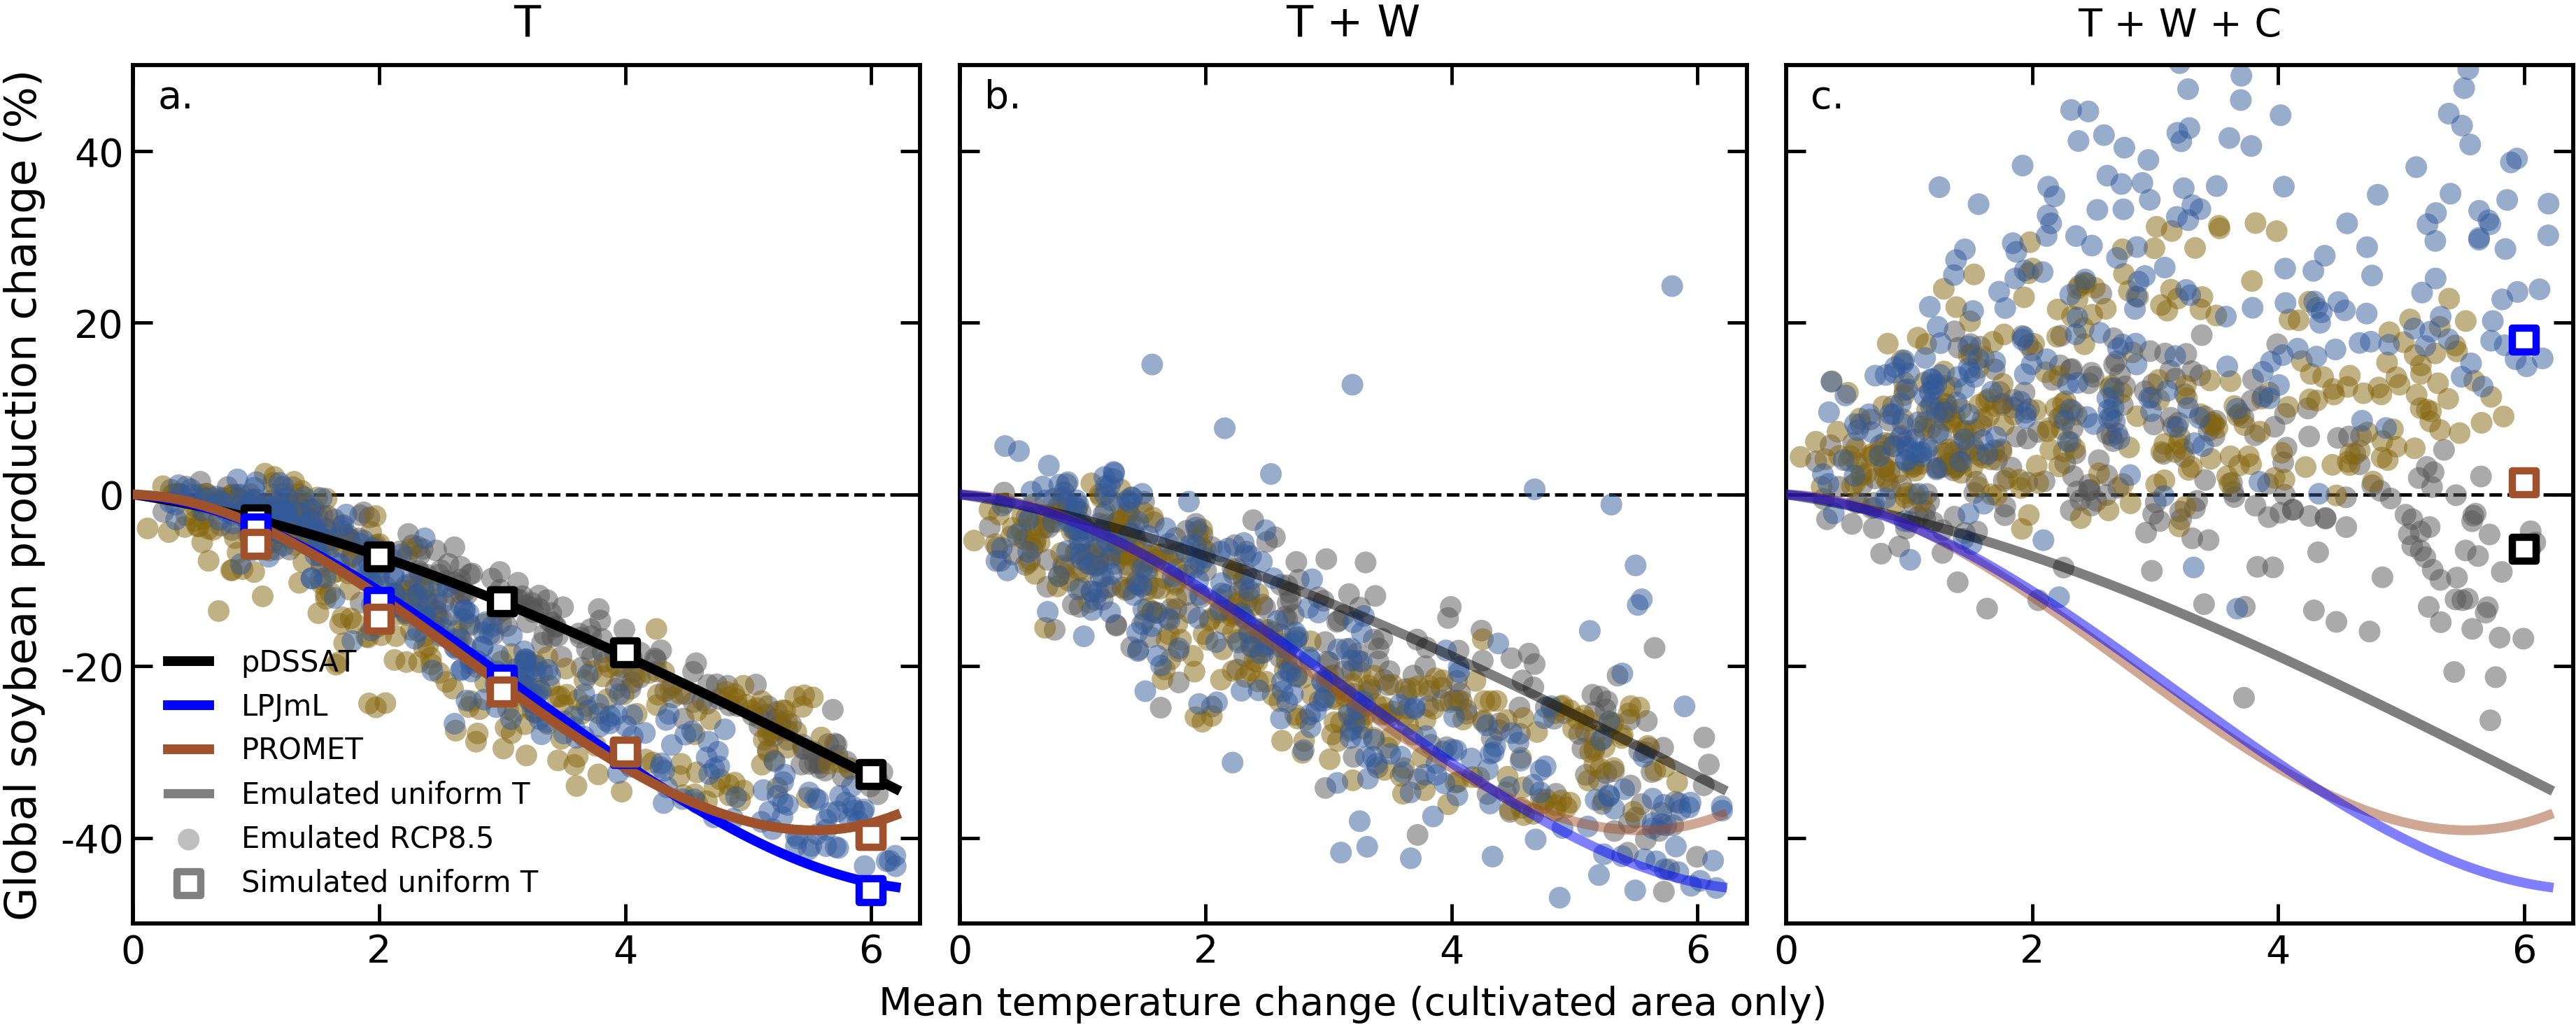
\includegraphics[width = 16.3cm]{LPJmL_pDSSAT_PROMET_RCP85_all_cases_soy.png}
  \caption{
  Illustration of the factors affecting yields in more realistic climate scenarios for soy. Same convention main text Figure 11.
  }
\end{figure}


\clearpage
\section{Reduced specification (23-term) emulator examples}
\smallskip
\begin{flushleft}
In this section we present some parallel figures for the reduced-form emulator (23-term). 
Issues with the reduced-form model are most prominent in PROMET for rice and soy, and JULES soy and spring wheat. 
Some potential causes behind this difference in ease of emulation are as follows.
First, we do not emulate PROMET or JULES in the nitrogen dimension (CARAIB is the other model that does not do N). 
Both JULES and PROMET models are land system process models, originally developed with a broad focus, and have relatively recently (2015) been adapted for managed vegetation (i.e. agriculture).
PROMET is the most sensitive model of all the models for rice in C, T, and W. 
PROMET is the quantitatively lowest performing model for soybeans when compared to the historical FAO data for the top 10 producing countries. 
JULES is the most sensitive model of all the models for soybeans in C, T, and W. 
For spring wheat, JULES is a high outlier in C, the most sensitive model in W and T, and shows an extra inflection point in the global temperature response not seen in any of the other models. 
CARAIB on the other hand (the other model that does not do nitrogen), was originally developed as a vegetation model in the early 90's and has a longer history of agricultural focus. It is the least sensitive model in T for rice and spring wheat, and is nearest to the ensemble mean in maize and winter wheat. 
In W, it is the least sensitive model for maize, and the wheats, the second least sensitive model for soybeans, and nearest to the ensemble mean for rice. 
For C, it is the nearest to the ensemble mean for the wheats and soy and unremarkable for rice. 
However, CARAIB is the most sensitive model for maize in the C dimension (though this is relatively less sensitive than most other responses for other models the other crops).
\end{flushleft}

\begin{figure}[h!]
  \centering
  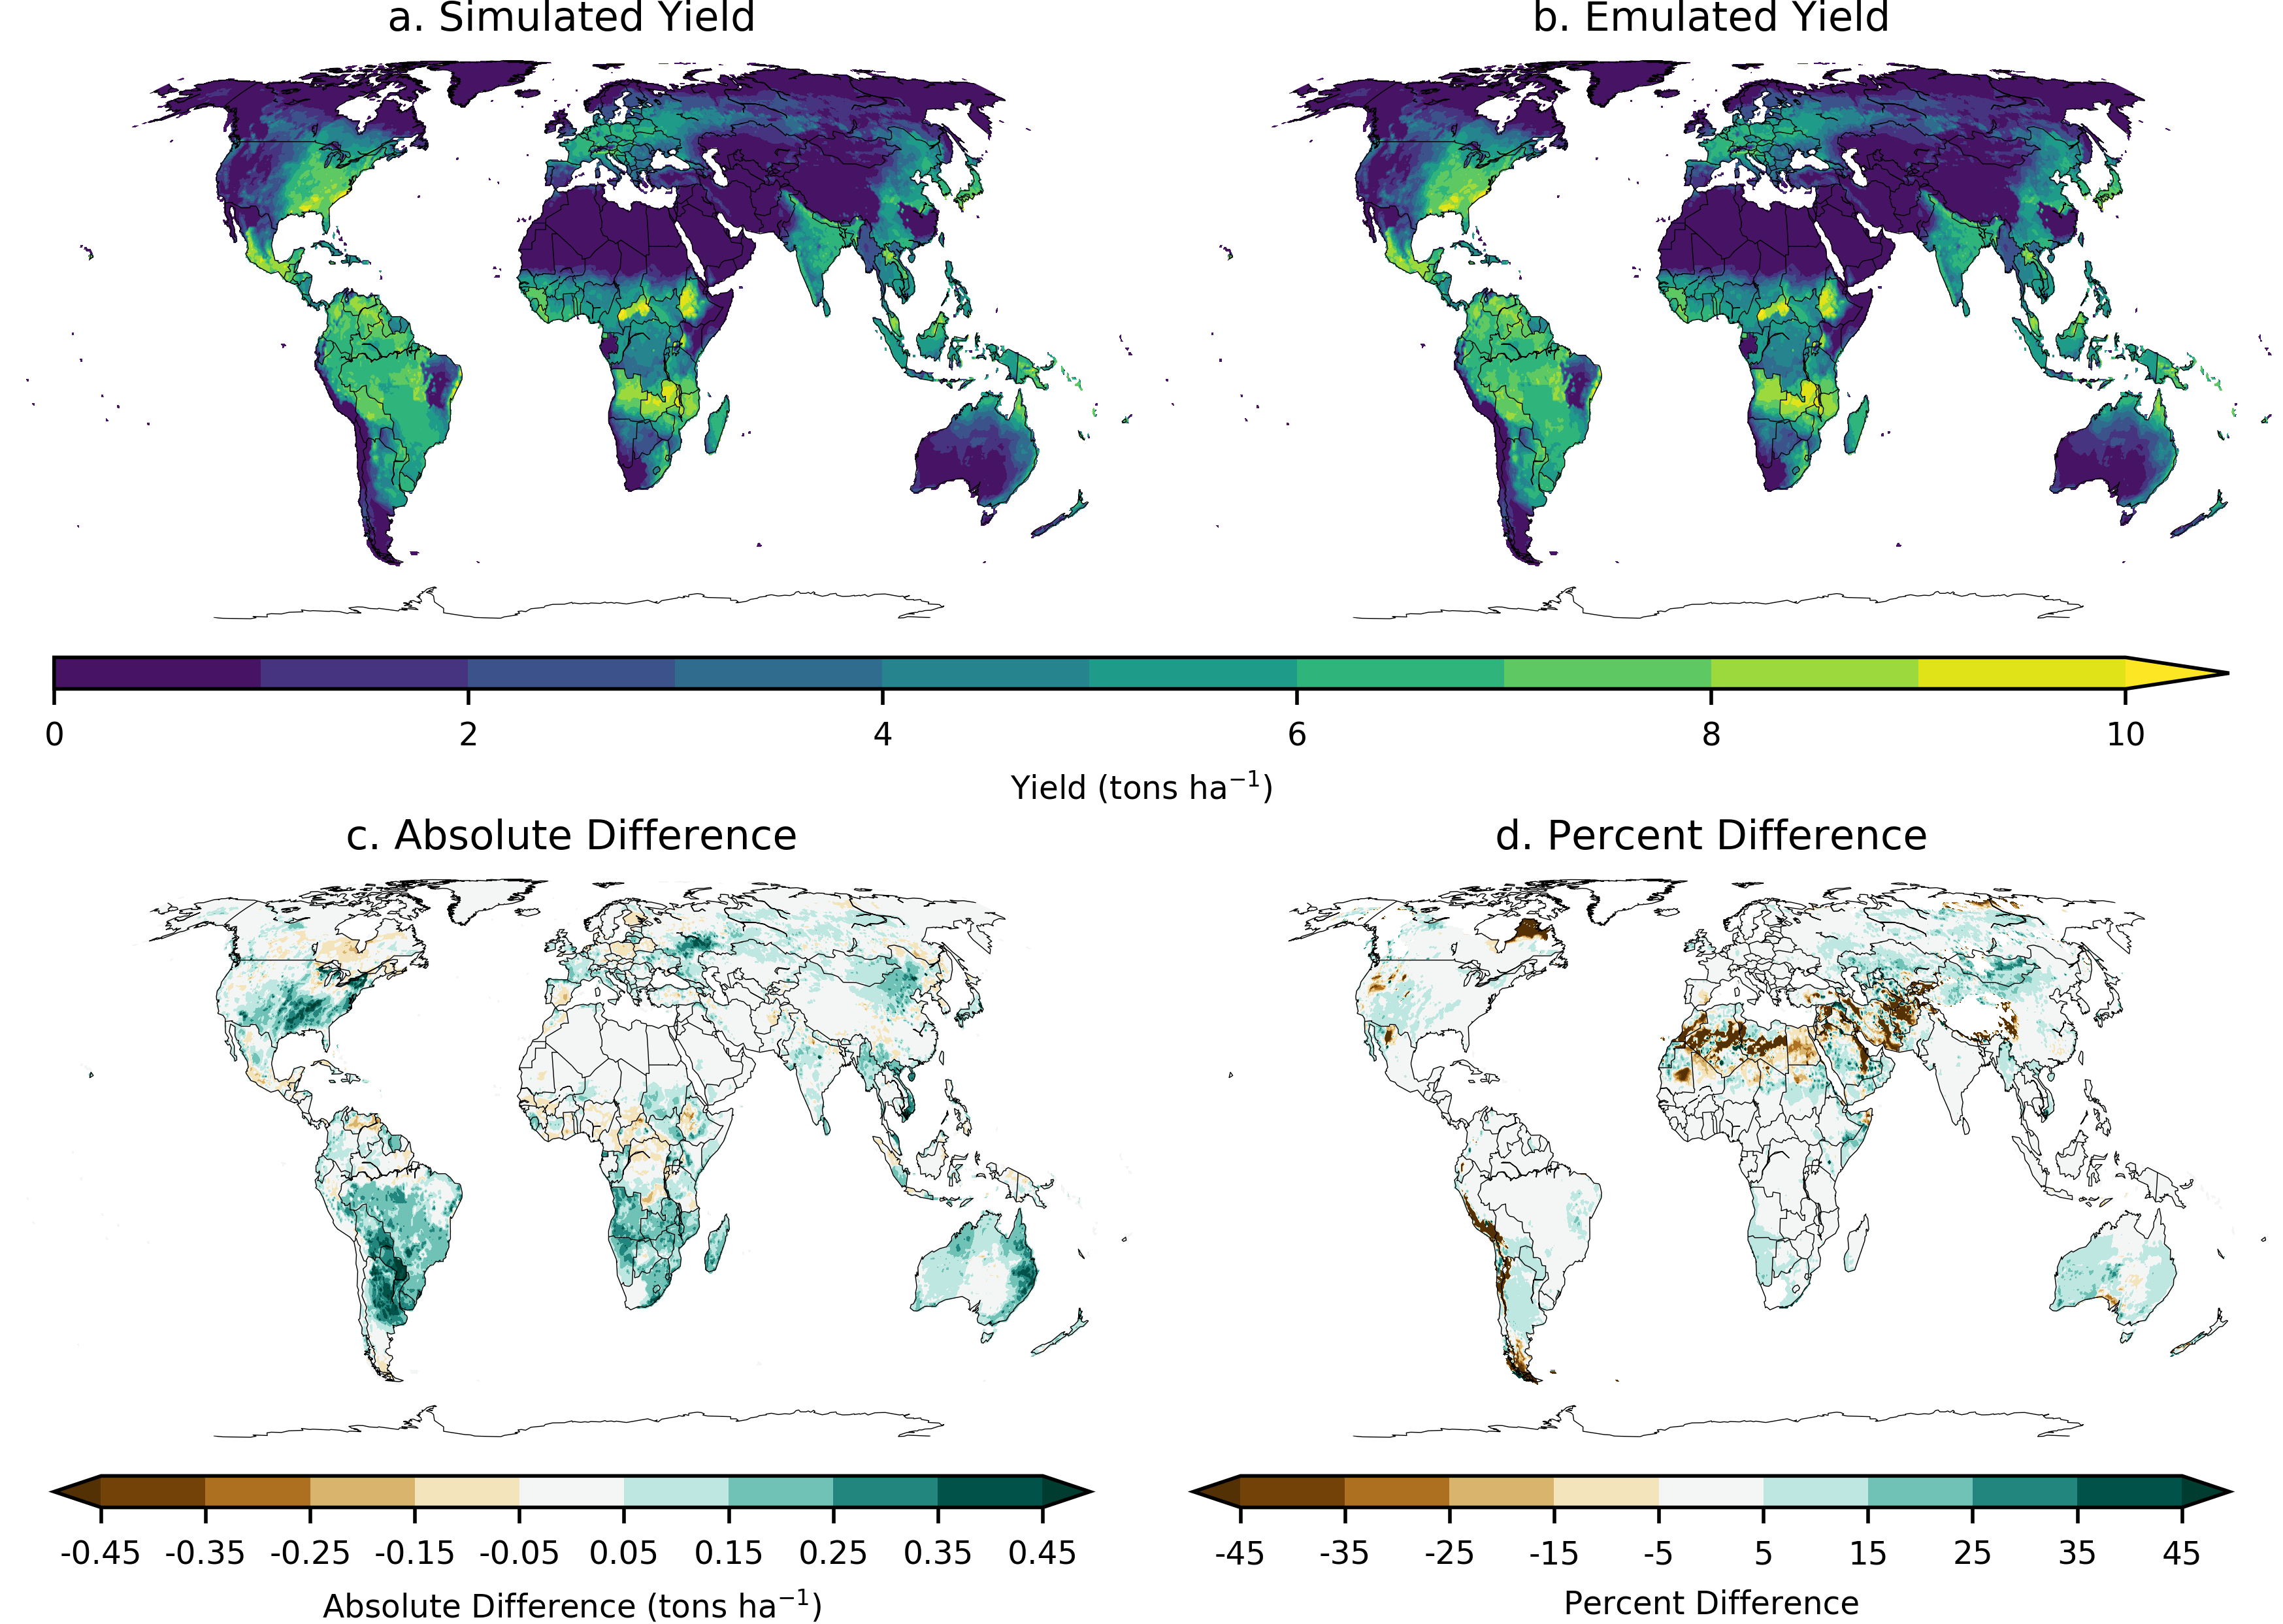
\includegraphics[width=15.5cm]{reduced_lpjml_maize.png}
  \caption{Same convention as Figure 4 in the main text except now with the reduced (23-term) emulator specification.}
  \label{fig:reducedlpjml}
\end{figure}

\begin{figure}[h!]
  \centering
  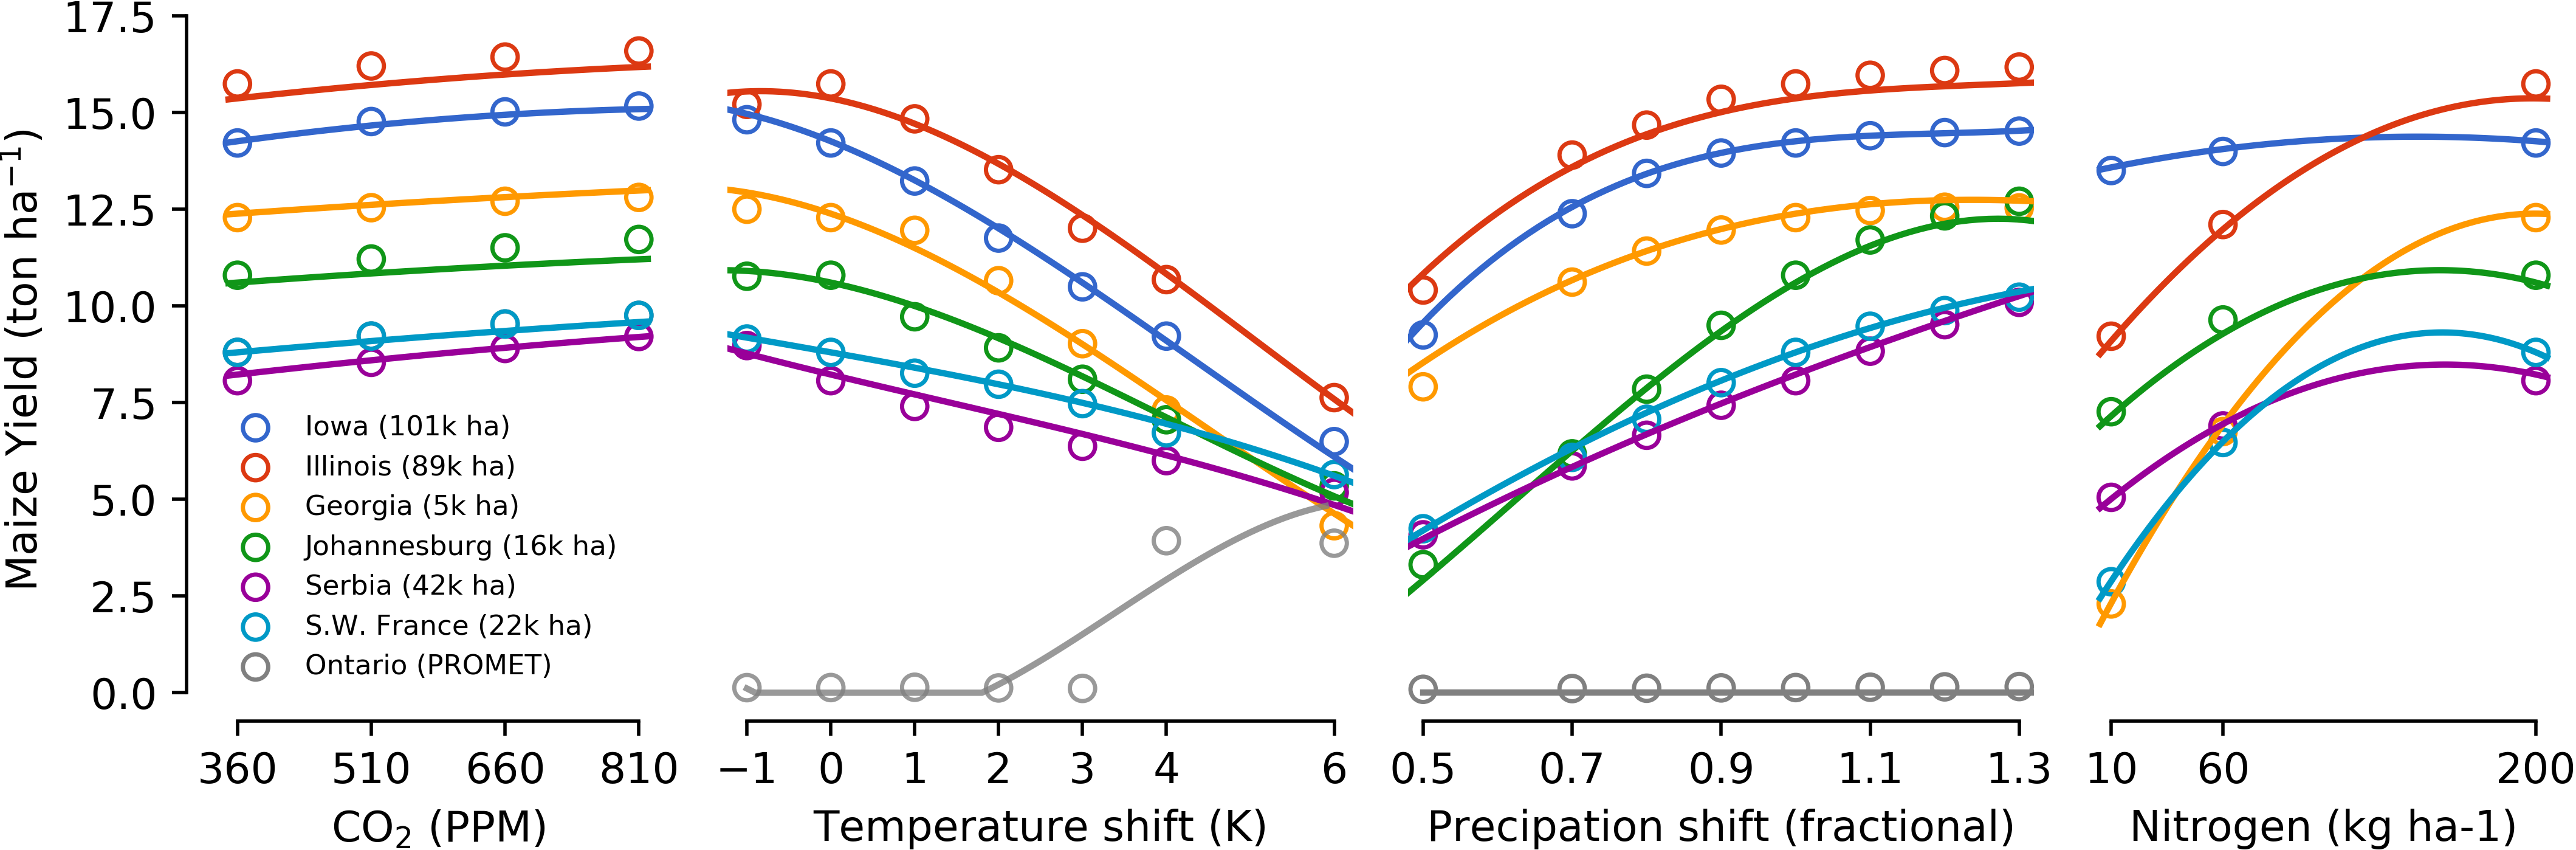
\includegraphics[width=15.5cm]{reduced_regression_example_1.png}
  \caption{Same convention as Figure 5 in the main text except now with the reduced (23-term) emulator specification.}
  \label{fig:reducedareas}
\end{figure}

\begin{figure}[h!]
  \centering
  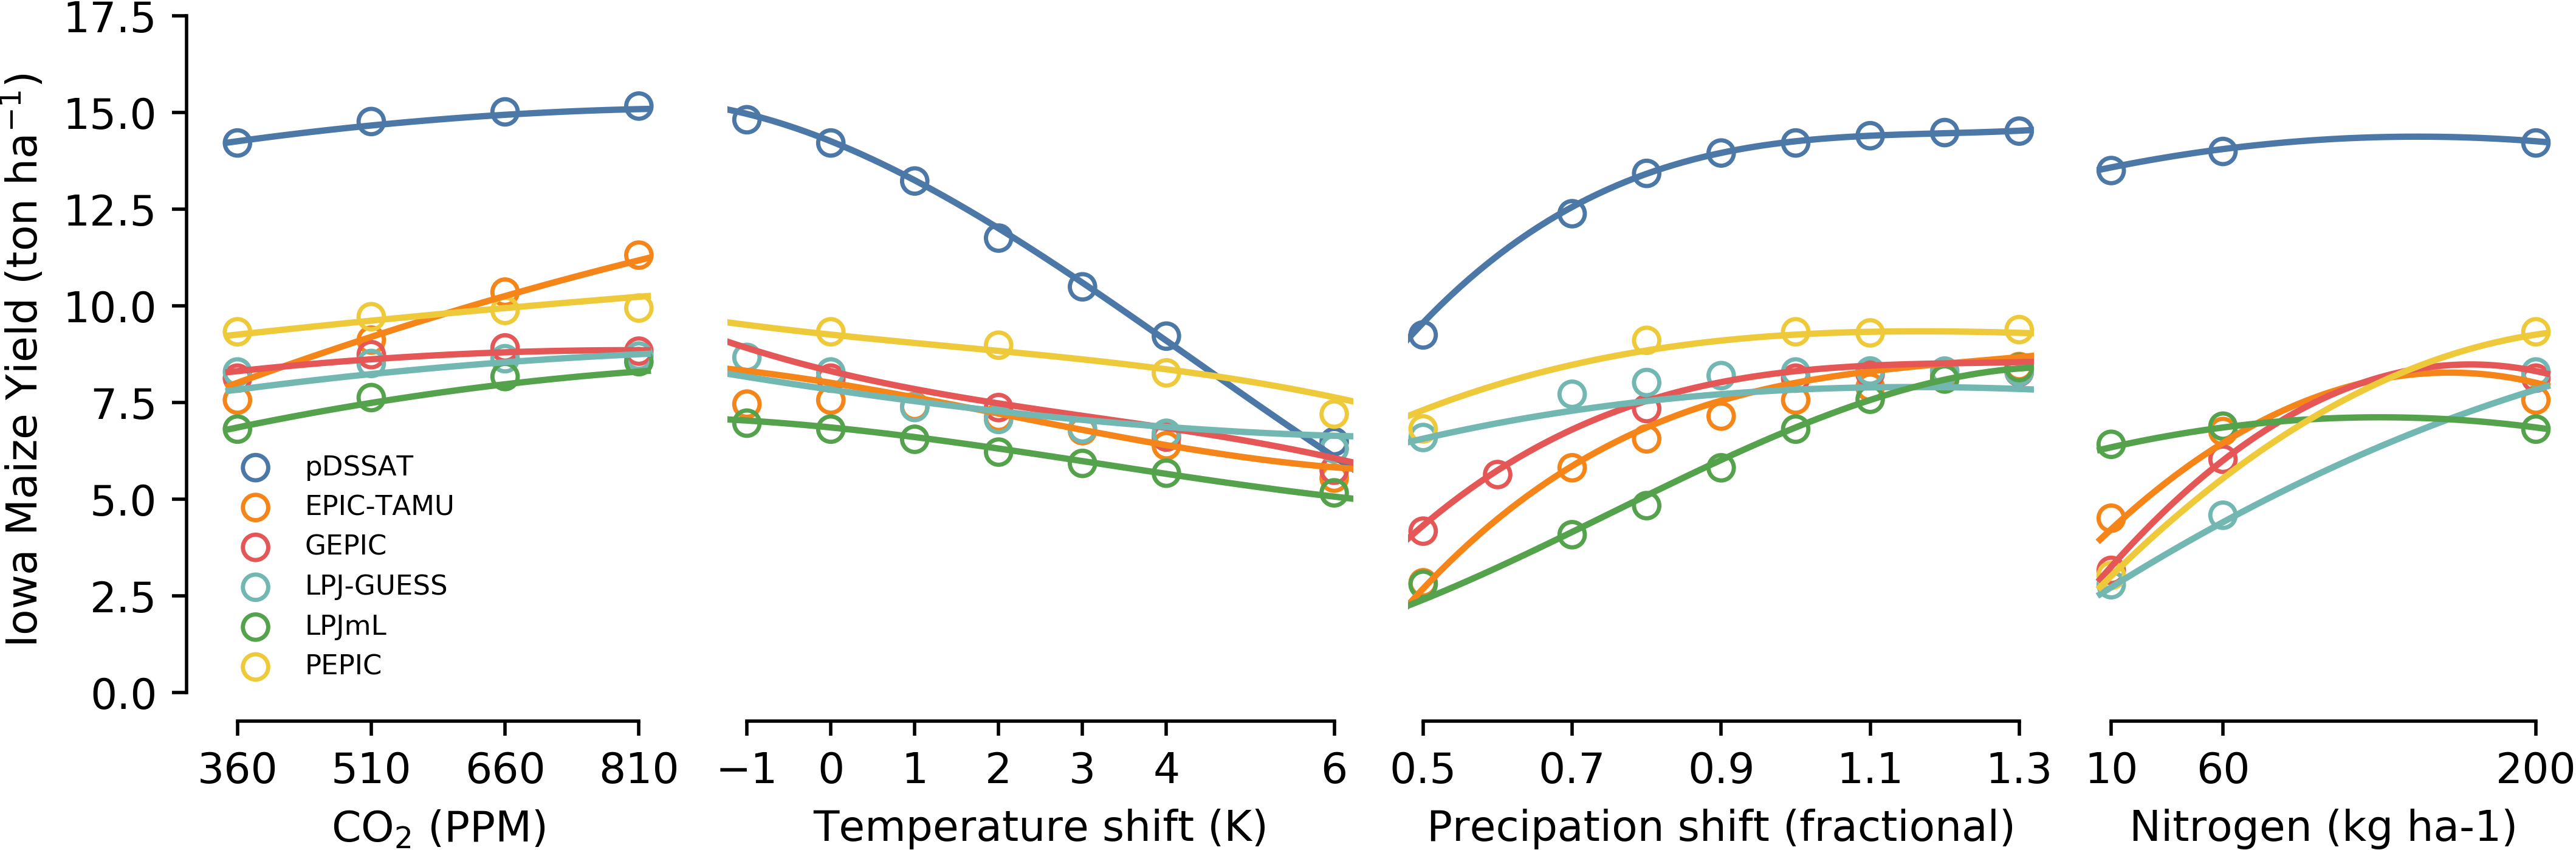
\includegraphics[width=15.5cm]{reduced_regression_example_2.png}
  \caption{Same convention as Figure 6 in the main text except now with the reduced (23-term) emulator specification.}
  \label{fig:reducedmodels}
\end{figure}

\begin{figure}[h!]
  \centering
  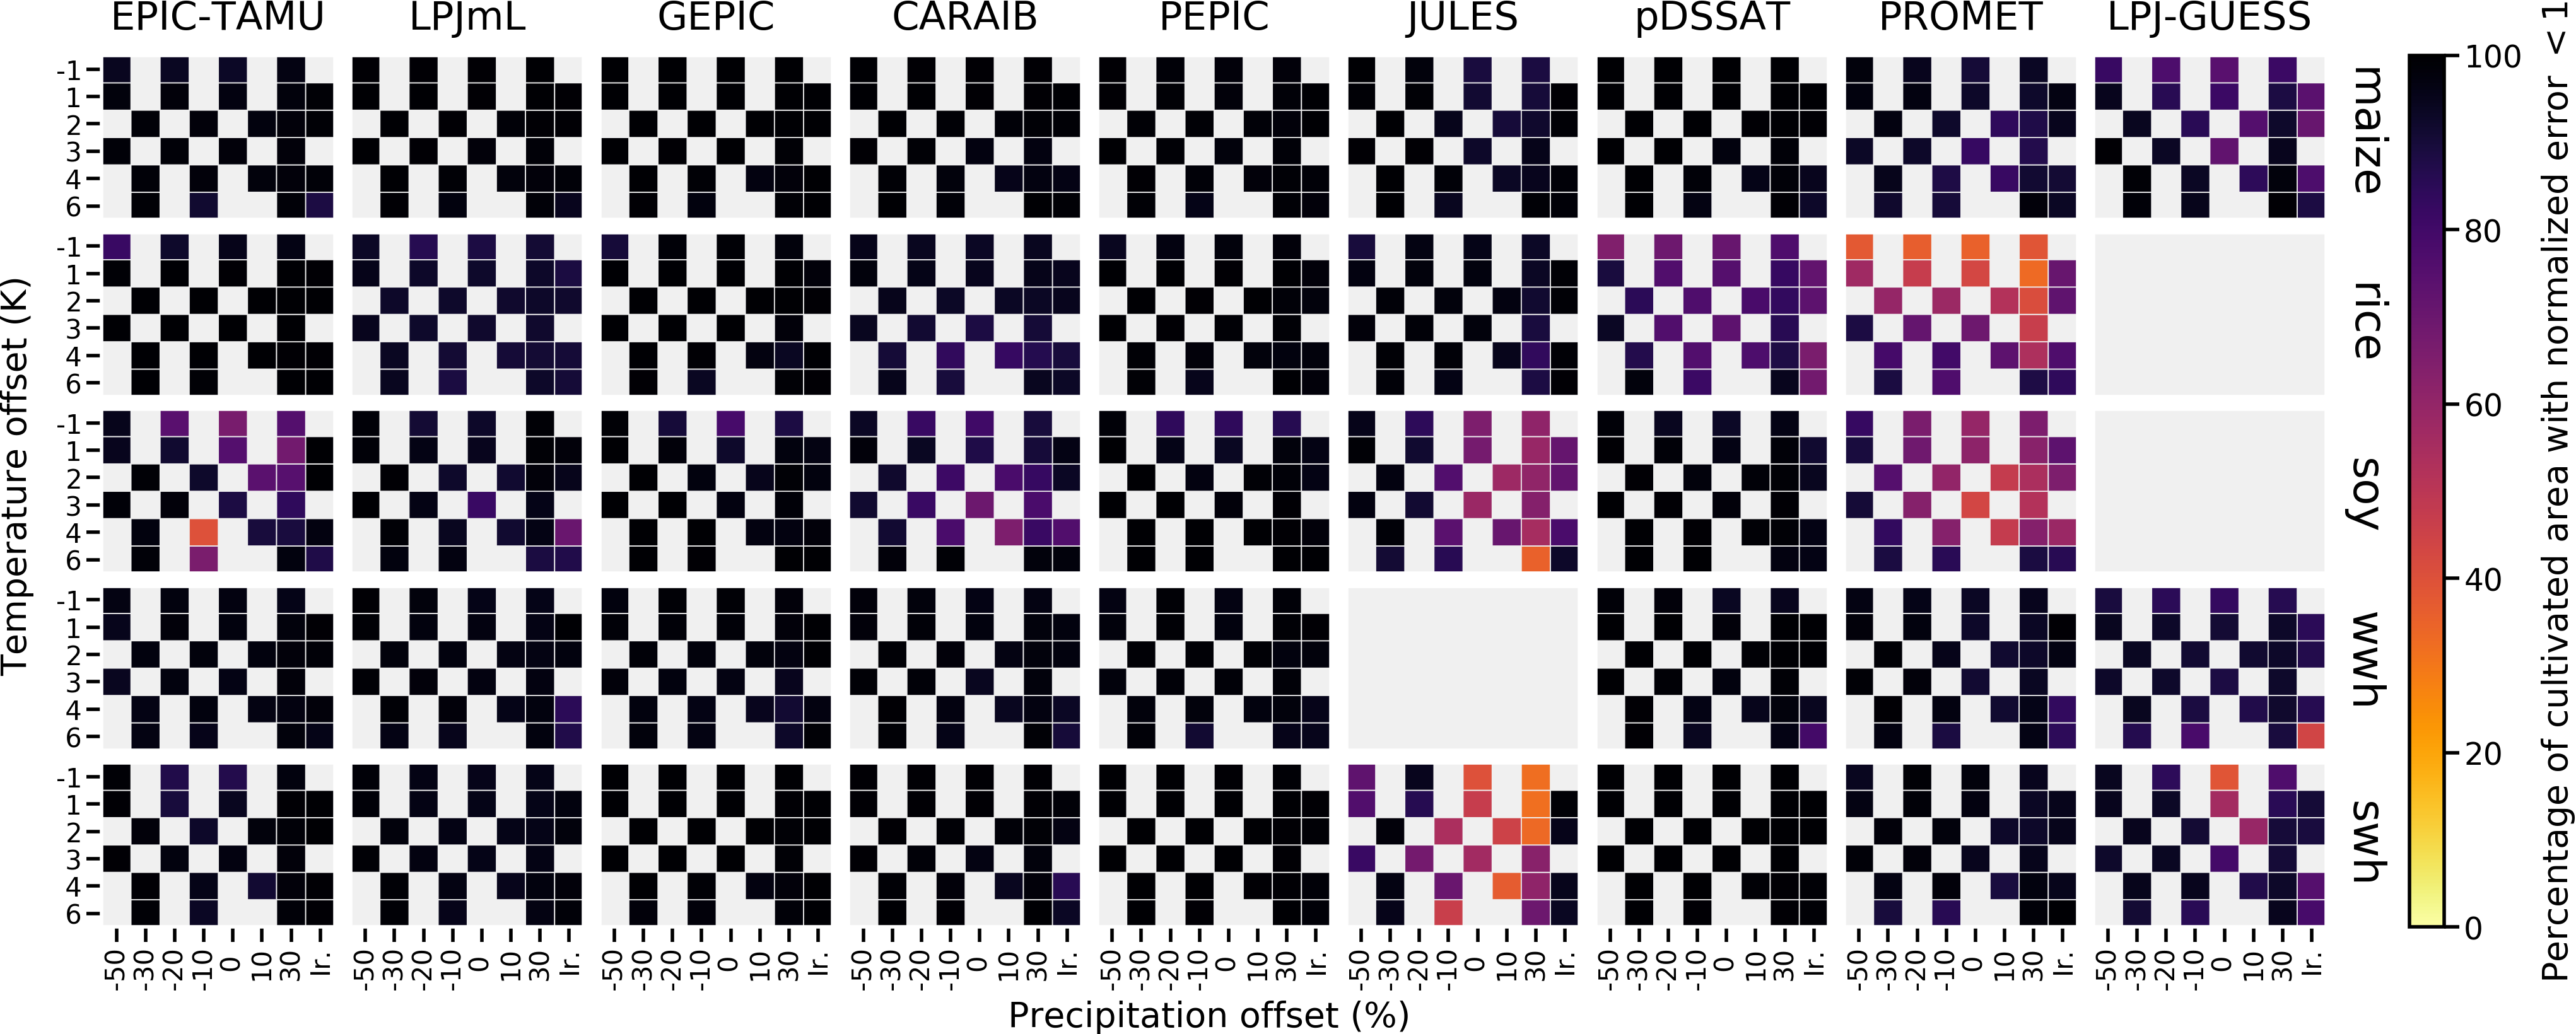
\includegraphics[width=15.5cm]{reduced_error_grid.png}
  \caption{
  Same convention as Figure 7 in the main text except now with the reduced (23-term) emulator specification.
  }
  \label{fig:reducedgrid}
\end{figure}

\begin{figure}[h!]
  \centering
  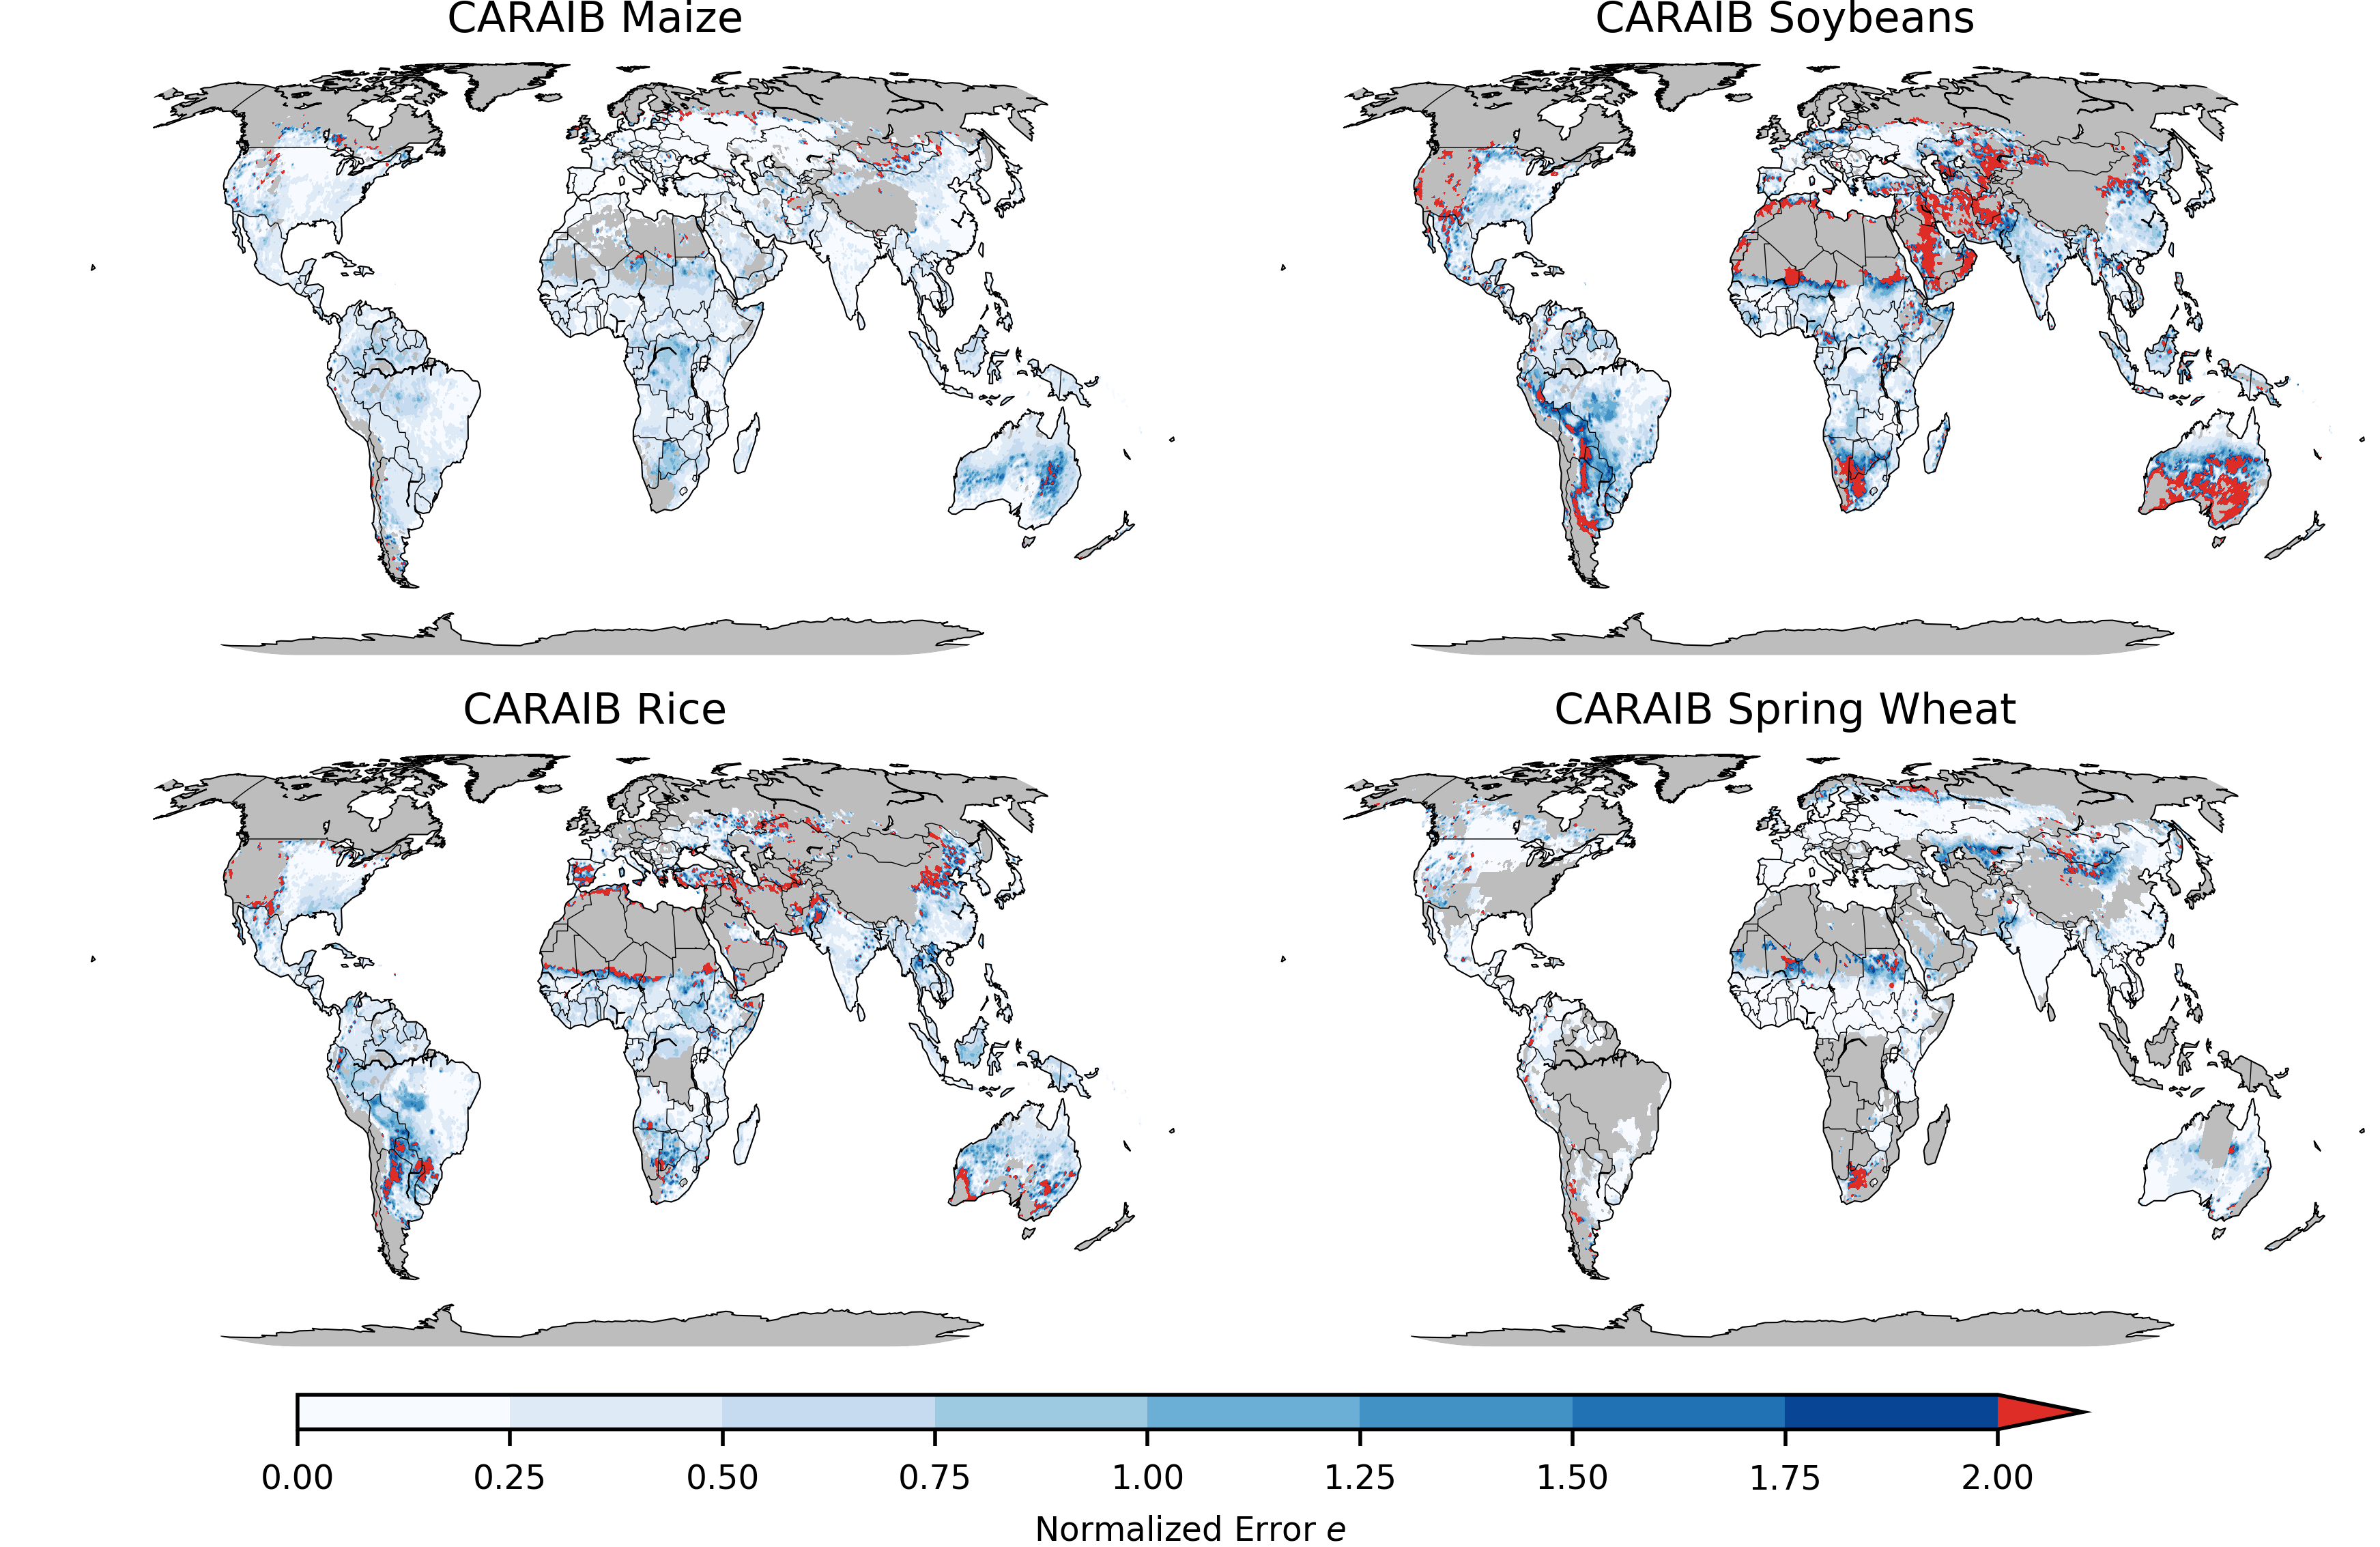
\includegraphics[width=15.5cm]{reduced_CARAIB_spatial_error.png}
  \caption{
  Same convention as Figure 8 in the main text except now with the reduced (23-term) emulator specification.
  }
  \label{fig:reducedcaraib}
\end{figure}

\begin{figure}[h!]
  \centering
  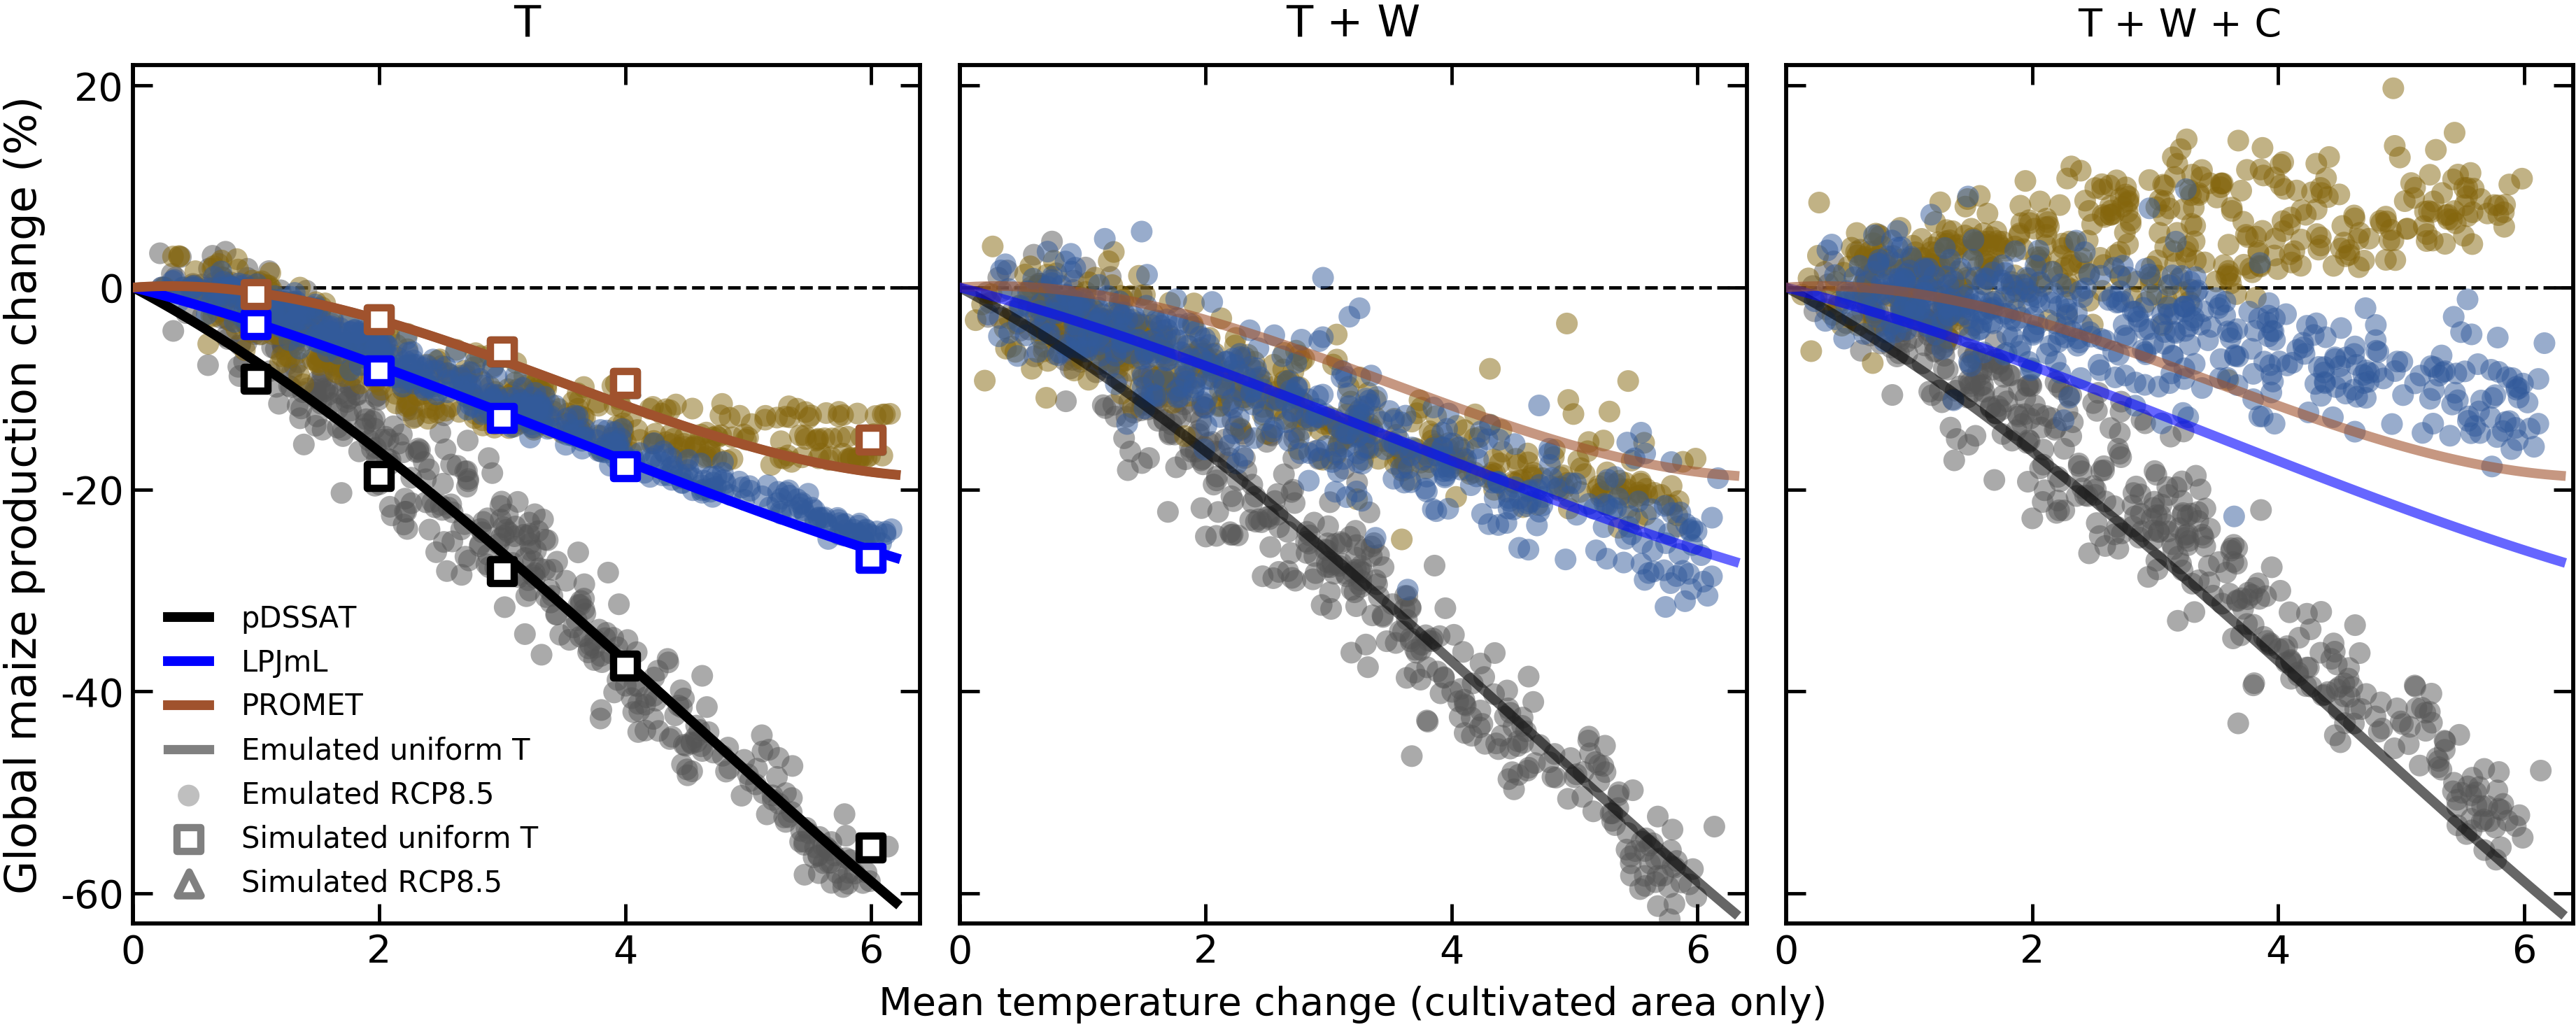
\includegraphics[width = 16.3cm]{reduced_global_em_maize.png}
  \caption{
  Same convention as Figure 11 in the main text except now with the reduced (23-term) emulator specification.
  }
\end{figure}

\begin{figure}[h!]
  \centering
  \includegraphics[width=14cm]{JULES_soy_bad.png}
  \caption{
  Example of emulator failure. 
  Simulated and emulated values for JULES soybean in Southern Germany. RMSE = 41\% of baseline yield for the reduced form (23-term) emulator.
  The downturn in yields as C and W increase can only be captured by the higher order C interaction terms. 
  }
  \label{fig:lpjmlrice}
\end{figure}

\begin{figure}[h!]
  \centering
  \includegraphics[width=14cm]{PROMET_rice_bad.png}
  \caption{
  Example of emulator failure. Simulated and emulated values for PROMET rice in Arunachal Pradesh. RMSE = 132\% of baseline yield for red (reduced fit).
  The step change in the yields around 0 K at higher water specifications cannot be captured by any third order polynomial. 
  Both emulator specifications fail in this example.
  }
  \label{fig:lpjmlrice}
\end{figure}

%%%%%%%%%%%%%%%%%%%%%%%%%%%%%%%%%%%%%%%%%%%%%%%%%%%%%%%%%%%%%%%%%%%%%%%%%%%%%%%%%%%%%%%%%%%%%%%%%%%%%%%%%%%%%%%%
%%%%%%%%%%%%%%%%%%%%%%%%%%%%%%%%%%%%%%%%%%%%%%%%%%%%%%%%%%%%%%%%%%%%%%%%%%%%%%%%%%%%%%%%%%%%%%%%%%%%%%%%%%%%%%%%
%%%%%%%%%%%%%%%%%%%%%%%%%%%%%%%%%%%%%%%%%%%%%%%%%%%%%%%%%%%%%%%%%%%%%%%%%%%%%%%%%%%%%%%%%%%%%%%%%%%%%%%%%%%%%%%%
%%%%%%%%%%%%%%%%%%%%%%%%%%%%%%%%%%%%%%%%%%%%%%%%%%%%%%%%%%%%%%%%%%%%%%%%%%%%%%%%%%%%%%%%%%%%%%%%%%%%%%%%%%%%%%%%
%%%%%%%%%%%%%%%%%%%%%%%%%%%%%%%%%%%%%%%%%%%            %%%%%%%%%%%%%%%%%%%%%%%%%%%%%%%%%%%%%%%%%%%%%%%%%%%%%%%%%
%%%%%%%%%%%%%%%%%%%%%%%%%%%%%%%%%%%%%%%%%%%   Part 2   %%%%%%%%%%%%%%%%%%%%%%%%%%%%%%%%%%%%%%%%%%%%%%%%%%%%%%%%%
%%%%%%%%%%%%%%%%%%%%%%%%%%%%%%%%%%%%%%%%%%%            %%%%%%%%%%%%%%%%%%%%%%%%%%%%%%%%%%%%%%%%%%%%%%%%%%%%%%%%%
%%%%%%%%%%%%%%%%%%%%%%%%%%%%%%%%%%%%%%%%%%%%%%%%%%%%%%%%%%%%%%%%%%%%%%%%%%%%%%%%%%%%%%%%%%%%%%%%%%%%%%%%%%%%%%%%
%%%%%%%%%%%%%%%%%%%%%%%%%%%%%%%%%%%%%%%%%%%%%%%%%%%%%%%%%%%%%%%%%%%%%%%%%%%%%%%%%%%%%%%%%%%%%%%%%%%%%%%%%%%%%%%%
%%%%%%%%%%%%%%%%%%%%%%%%%%%%%%%%%%%%%%%%%%%%%%%%%%%%%%%%%%%%%%%%%%%%%%%%%%%%%%%%%%%%%%%%%%%%%%%%%%%%%%%%%%%%%%%%
%%%%%%%%%%%%%%%%%%%%%%%%%%%%%%%%%%%%%%%%%%%%%%%%%%%%%%%%%%%%%%%%%%%%%%%%%%%%%%%%%%%%%%%%%%%%%%%%%%%%%%%%%%%%%%%%
%%%%%%%%%%%%%%%%%%%%%%%%%%%%%%%%%%%%%%%%%%%%%%%%%%%%%%%%%%%%%%%%%%%%%%%%%%%%%%%%%%%%%%%%%%%%%%%%%%%%%%%%%%%%%%%%

\clearpage
\section{Yield Responses for other crops and models}
\begin{figure}[h!]
  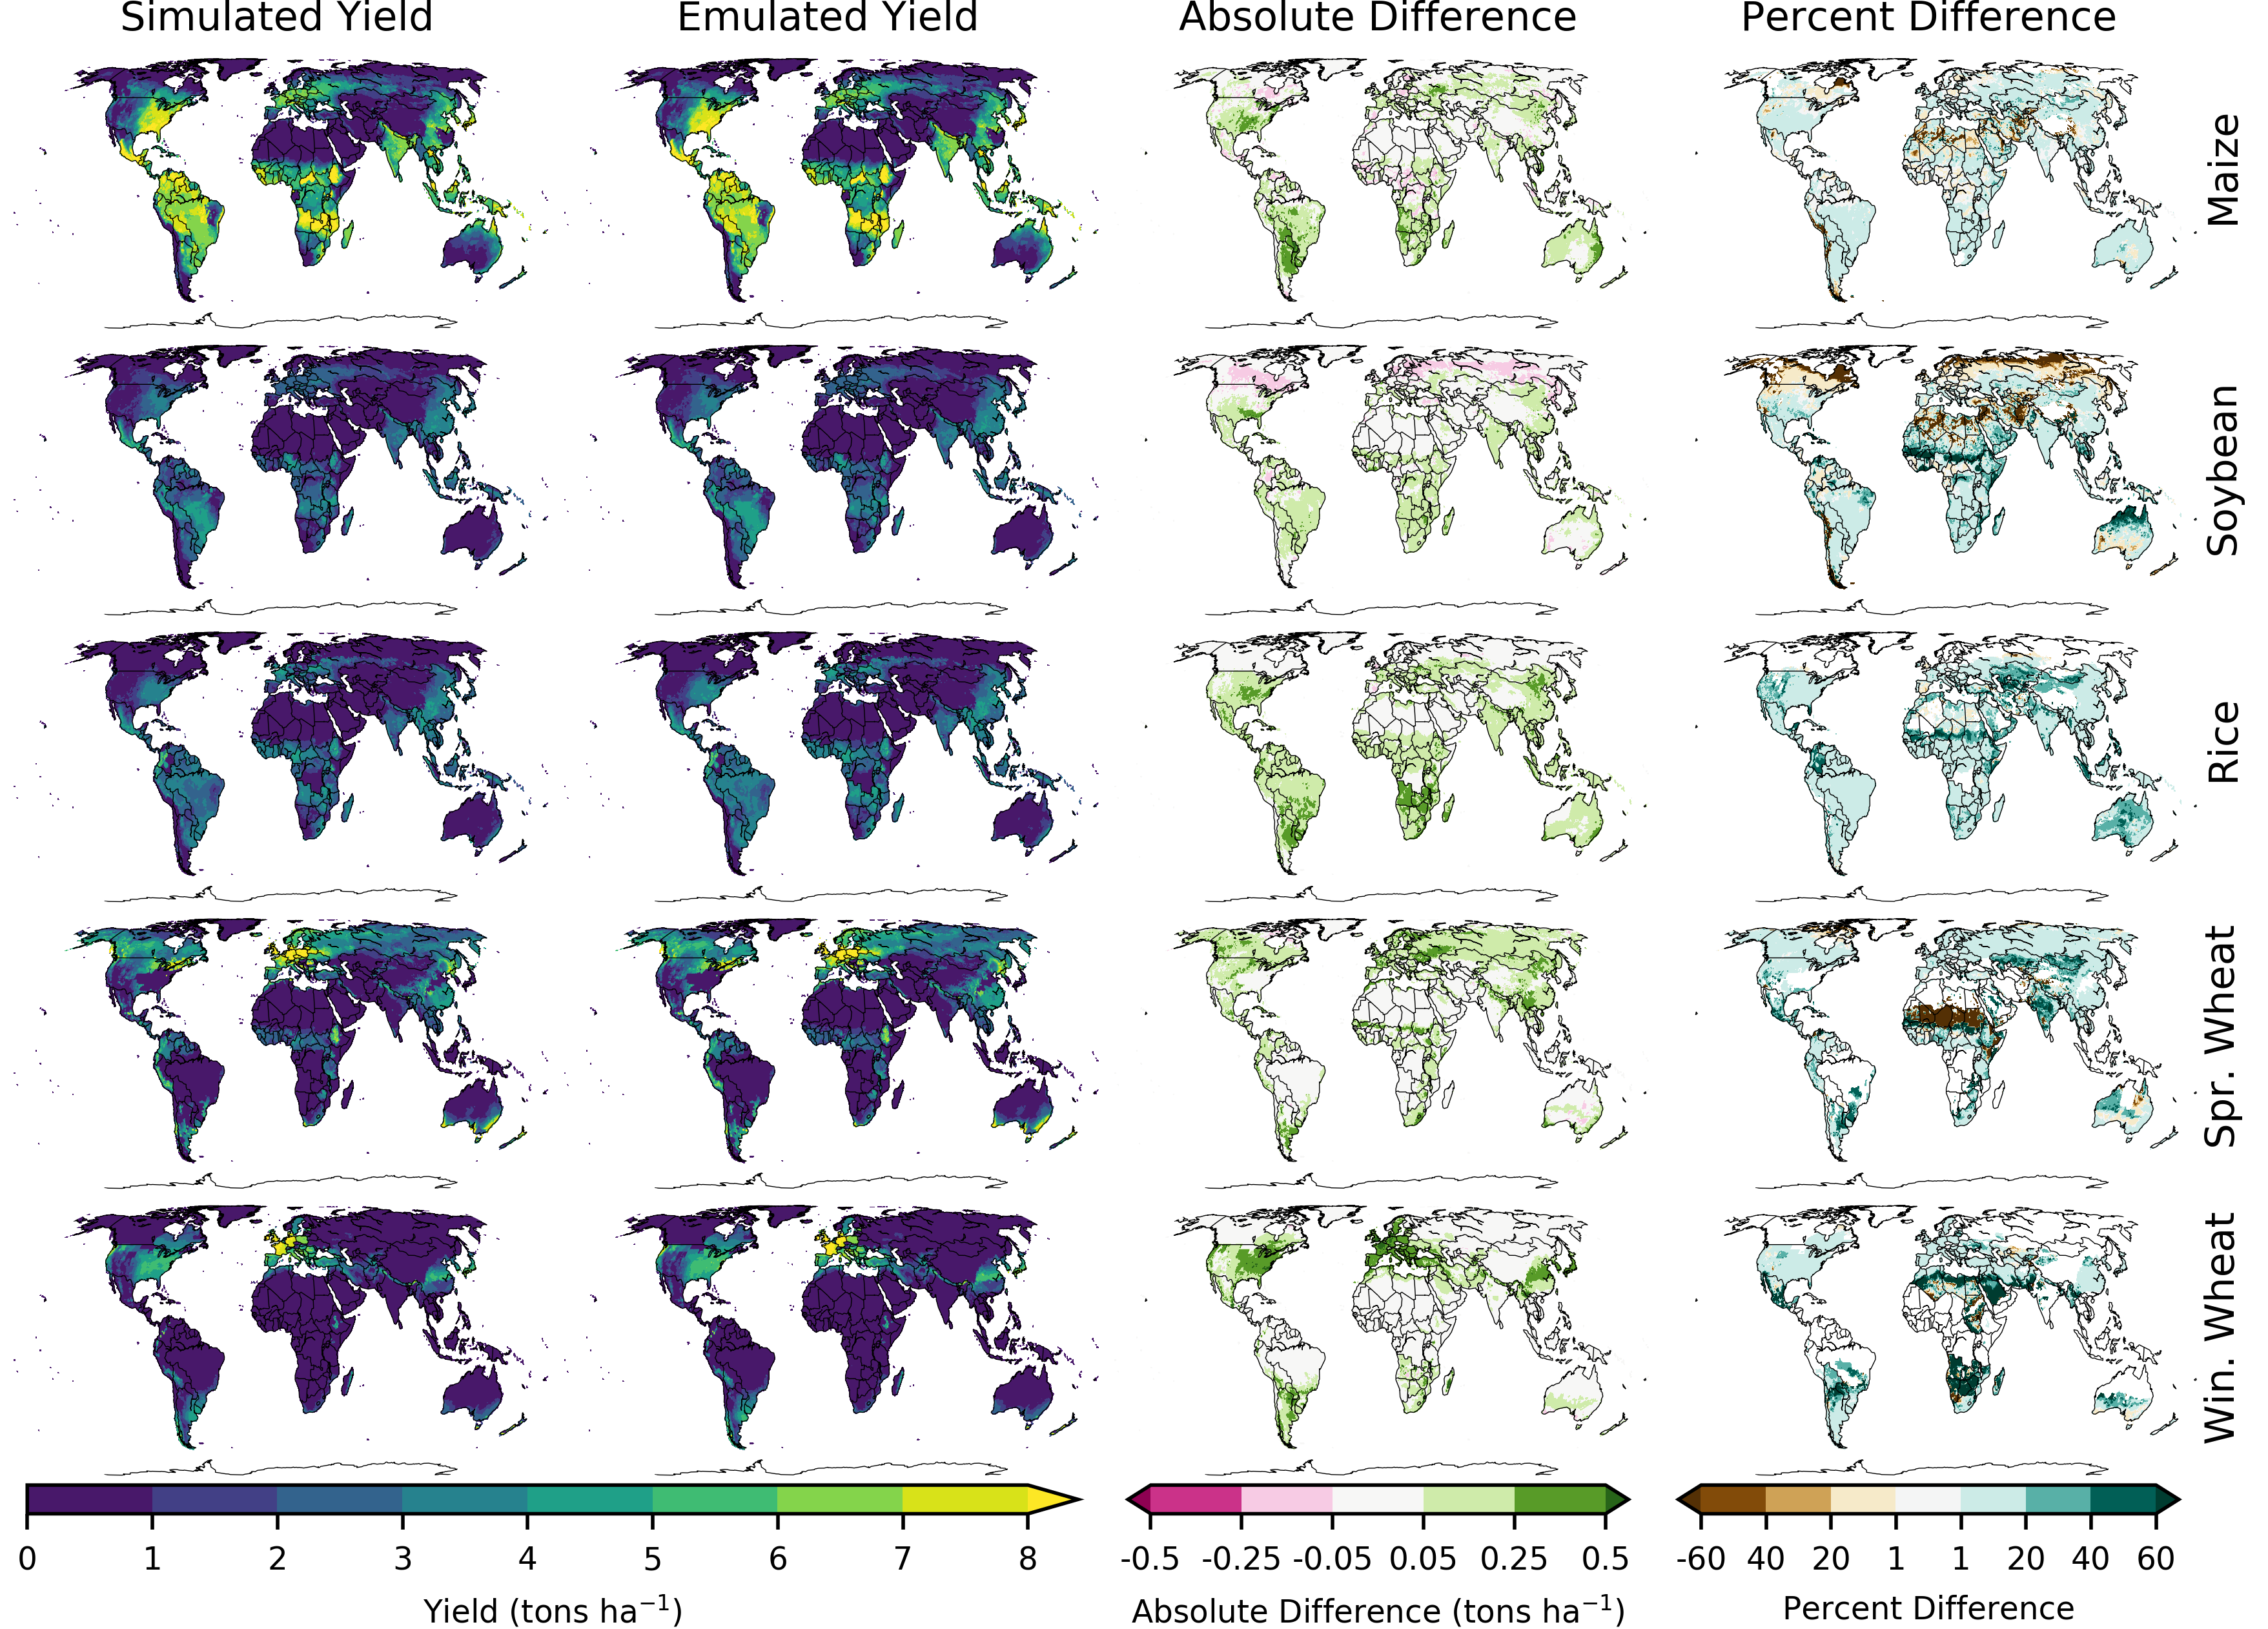
\includegraphics[width=\textwidth]{lpjml_grid.png}
  \caption{Spatial yield response and emulator error for LPJmL for all crops included in the stud. Same convention as Figure 4 in the main text.}
  \label{fig:lpjmlrice}
\end{figure}

\begin{figure}[h!]
  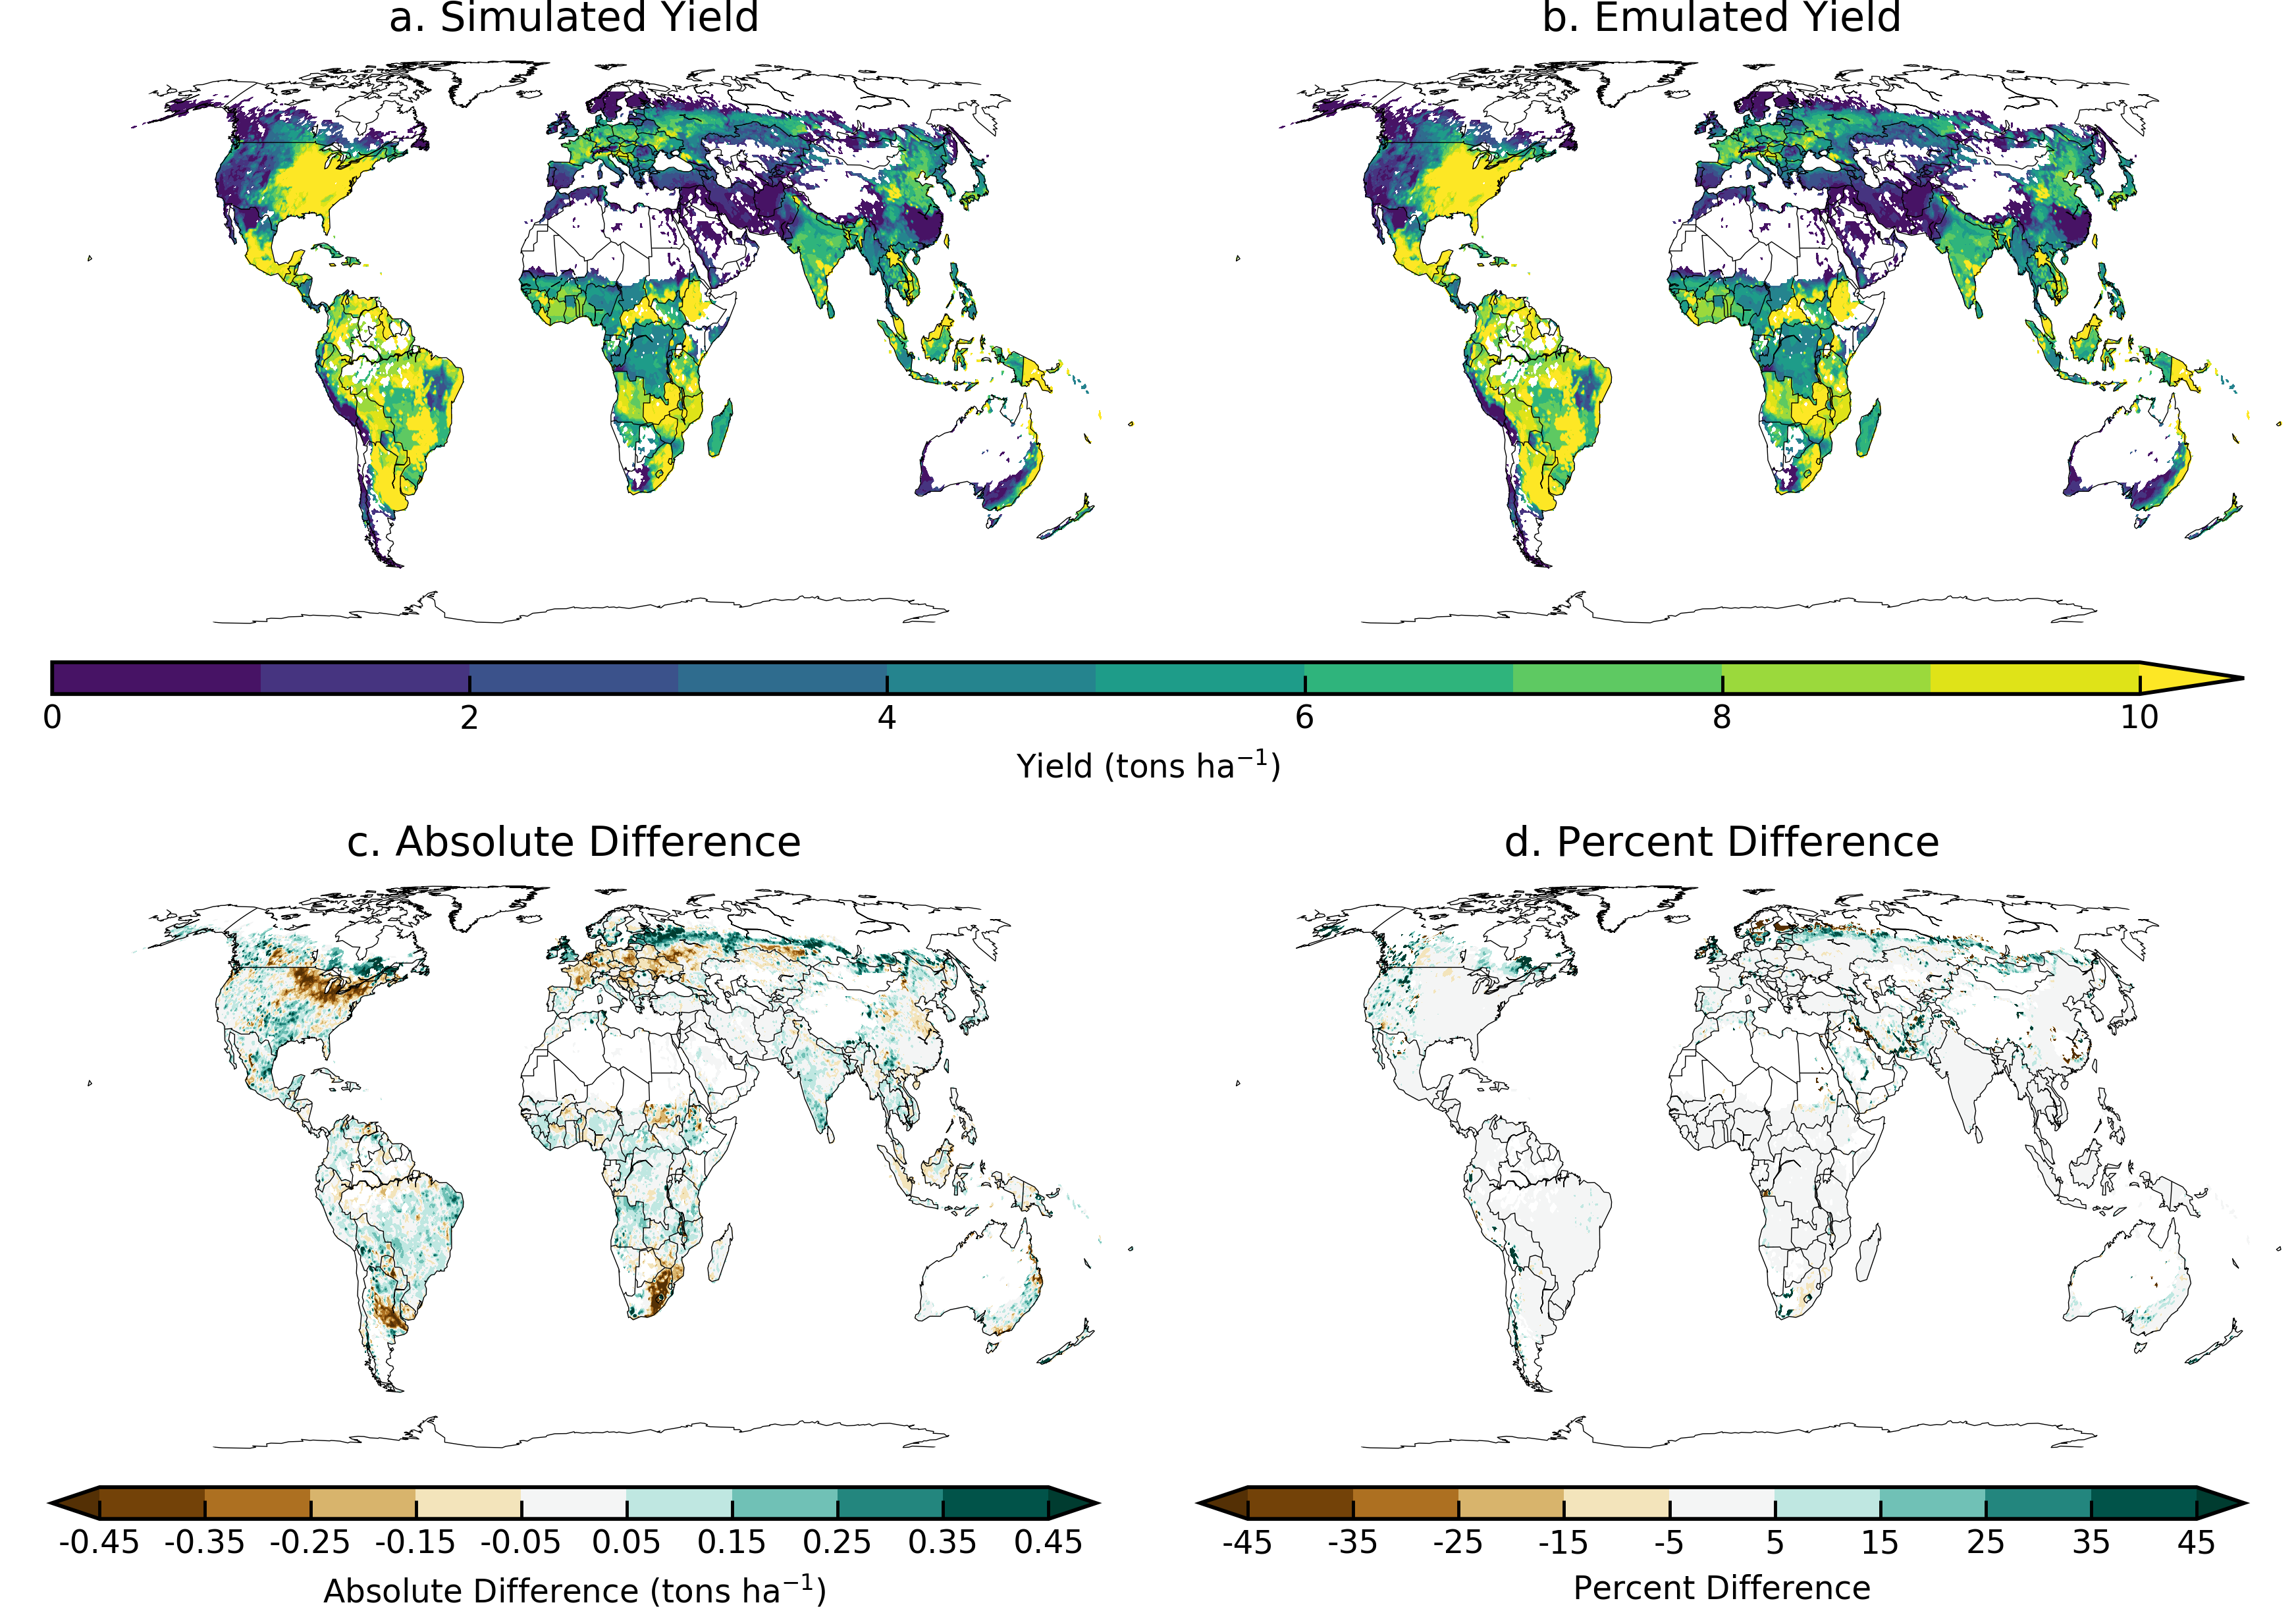
\includegraphics[width=\textwidth]{pdssat_maize.png}
  \caption{Spatial yield response and emulator error for pDSSAT for maize.Same convention as Figure 4 in the main text.}
  \label{fig:lpjmlrice}
\end{figure}

%%%%%%%%%%%%%%%%%%%%%%%%%%%%%%%%%%%%%%%%%%%%%%%%%%%%%%%%%%%%%%%%%%%%%%%%%%%%%%%%%%%%%%%
%%%%%%%%%%%%%%%%%%%%%%%%%%%%%%%%%%%%%%%%%%%%%%%%%%%%%%%%%%%%%%%%%%%%%%%%%%%%%%%%%%%%%%%
%%%%%%%%%%%%%%%%%%%%%%%%%%%%%%%%%%%%%%%%%%%%%%%%%%%%%%%%%%%%%%%%%%%%%%%%%%%%%%%%%%%%%%%

\clearpage
\section{Normalized Error for all models}

\begin{figure}[h!]
  \centering
  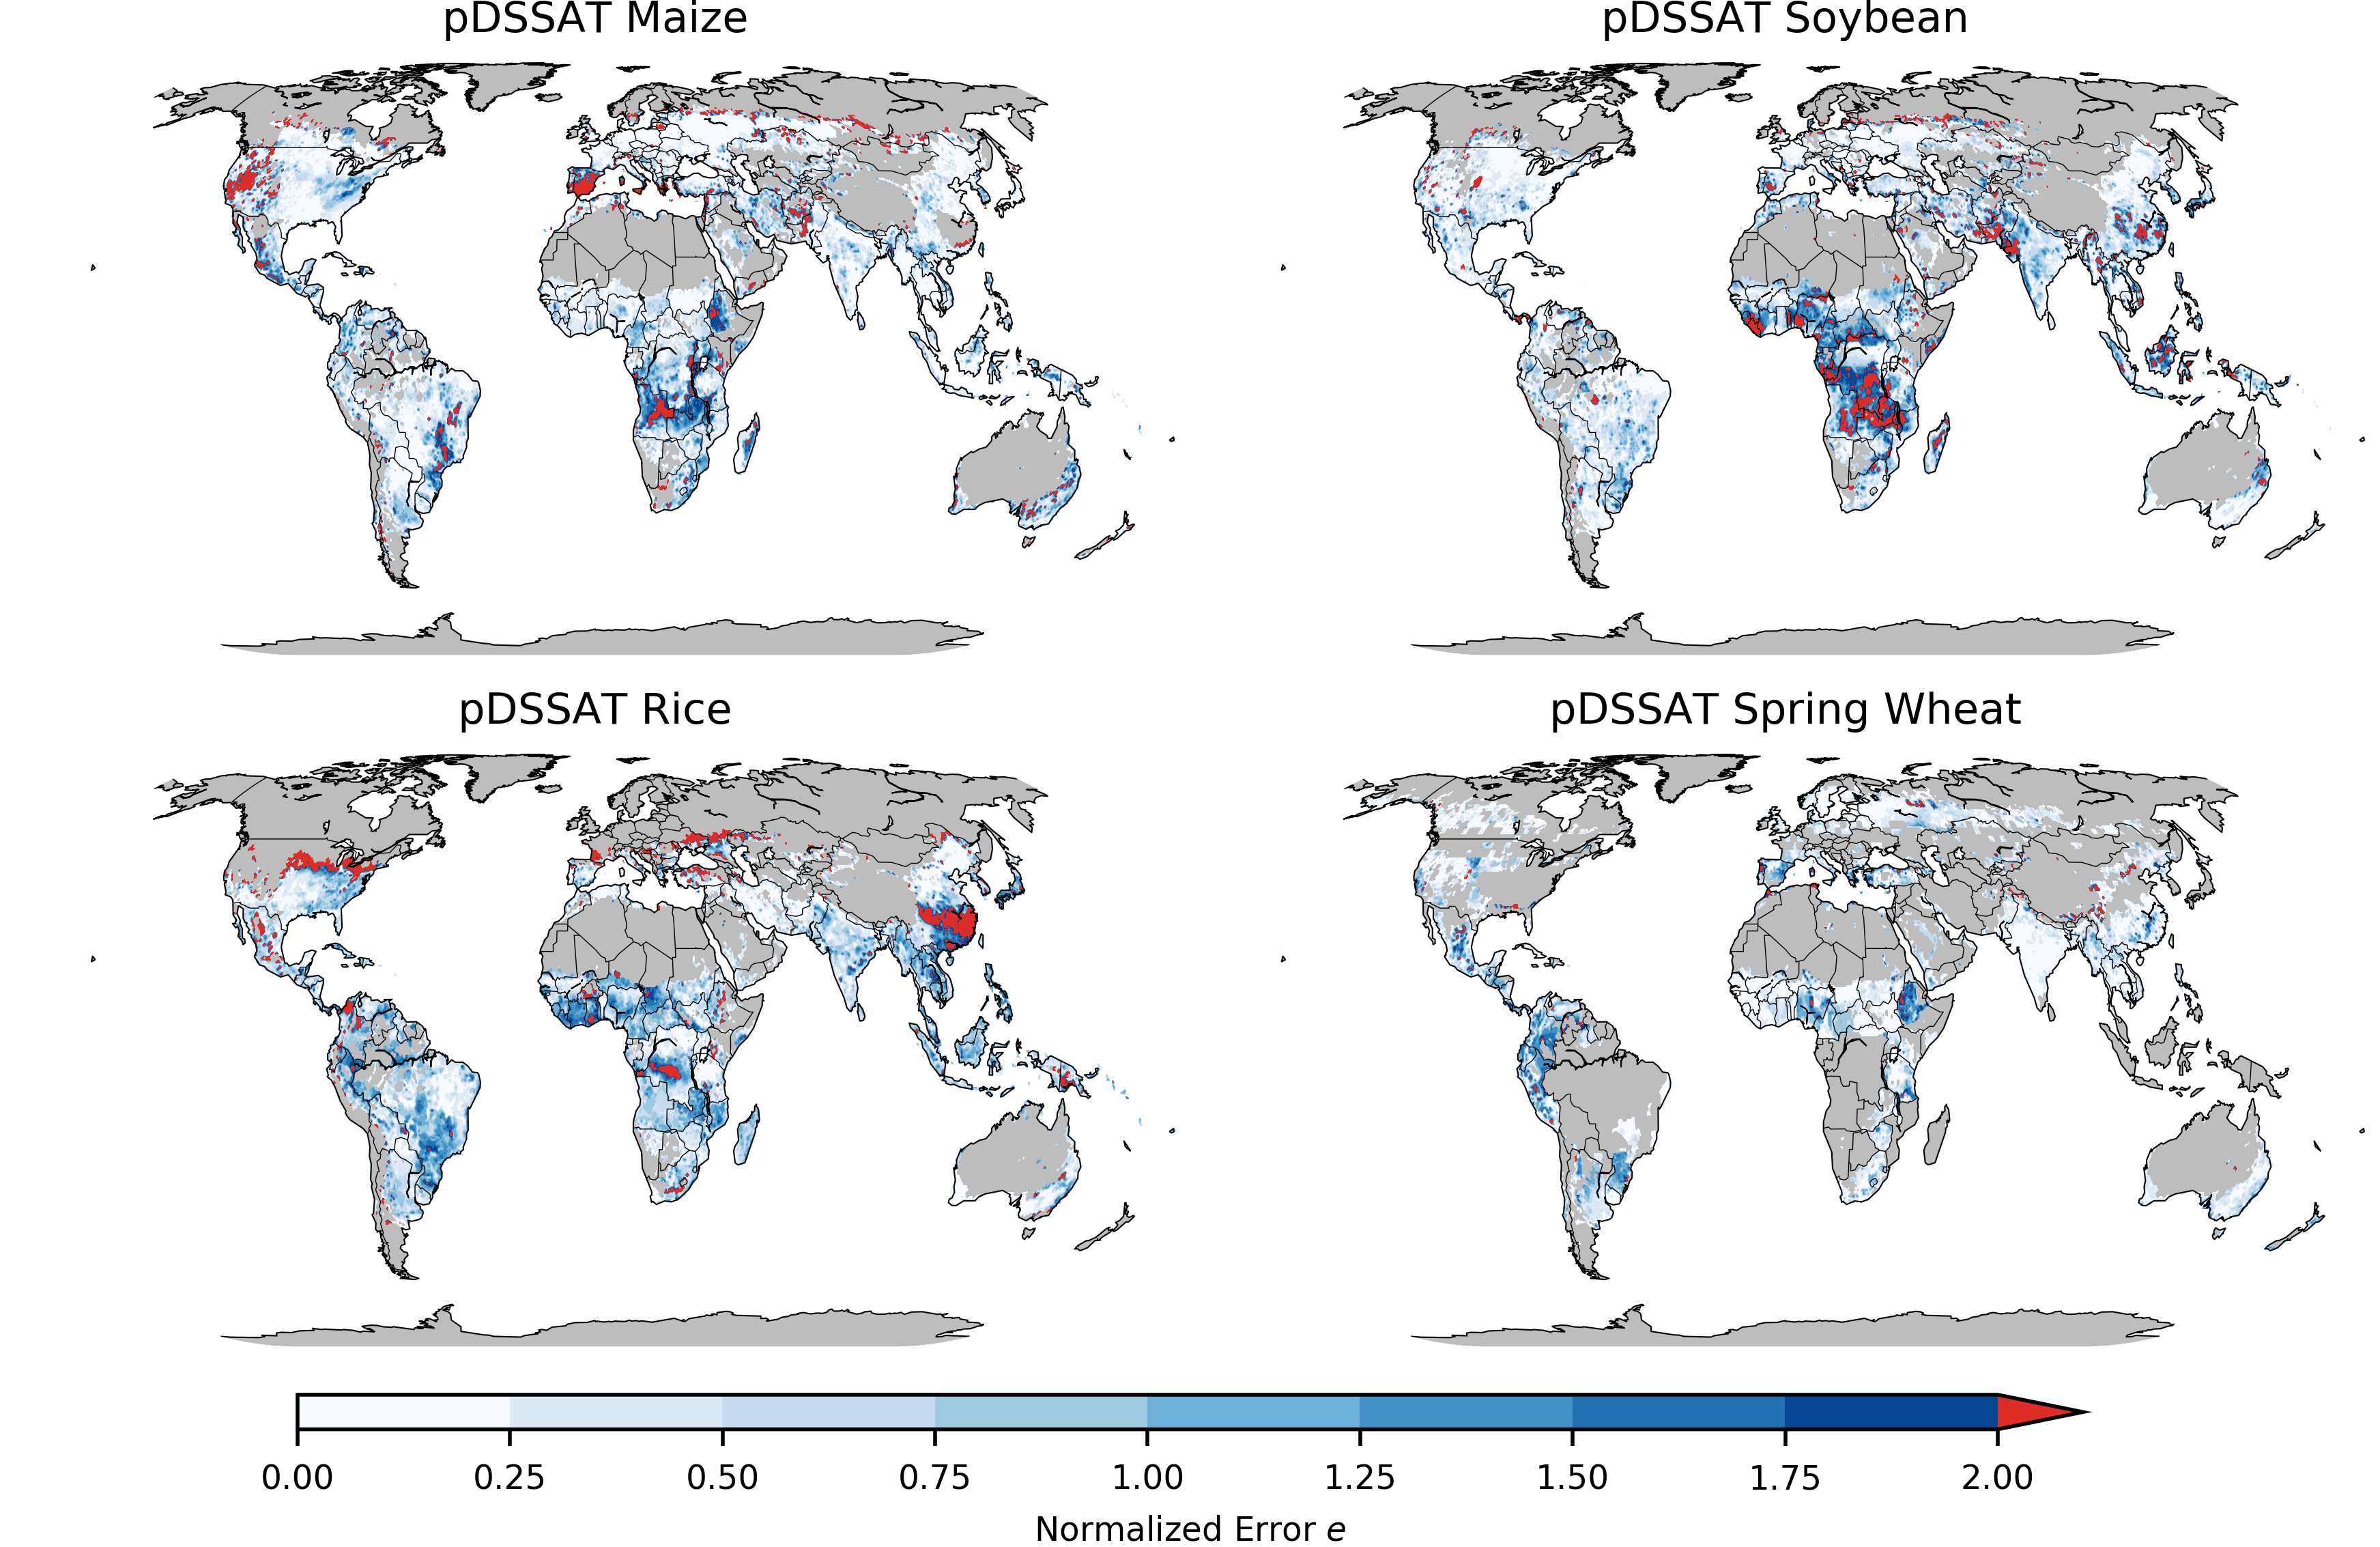
\includegraphics[width=15.5cm]{pDSSAT_spatial_error.png}
  \caption{Normalized error $e$ for pDSSAT. Same convention as main text Figure 8.}
\end{figure}

\begin{figure}[h!]
  \centering
  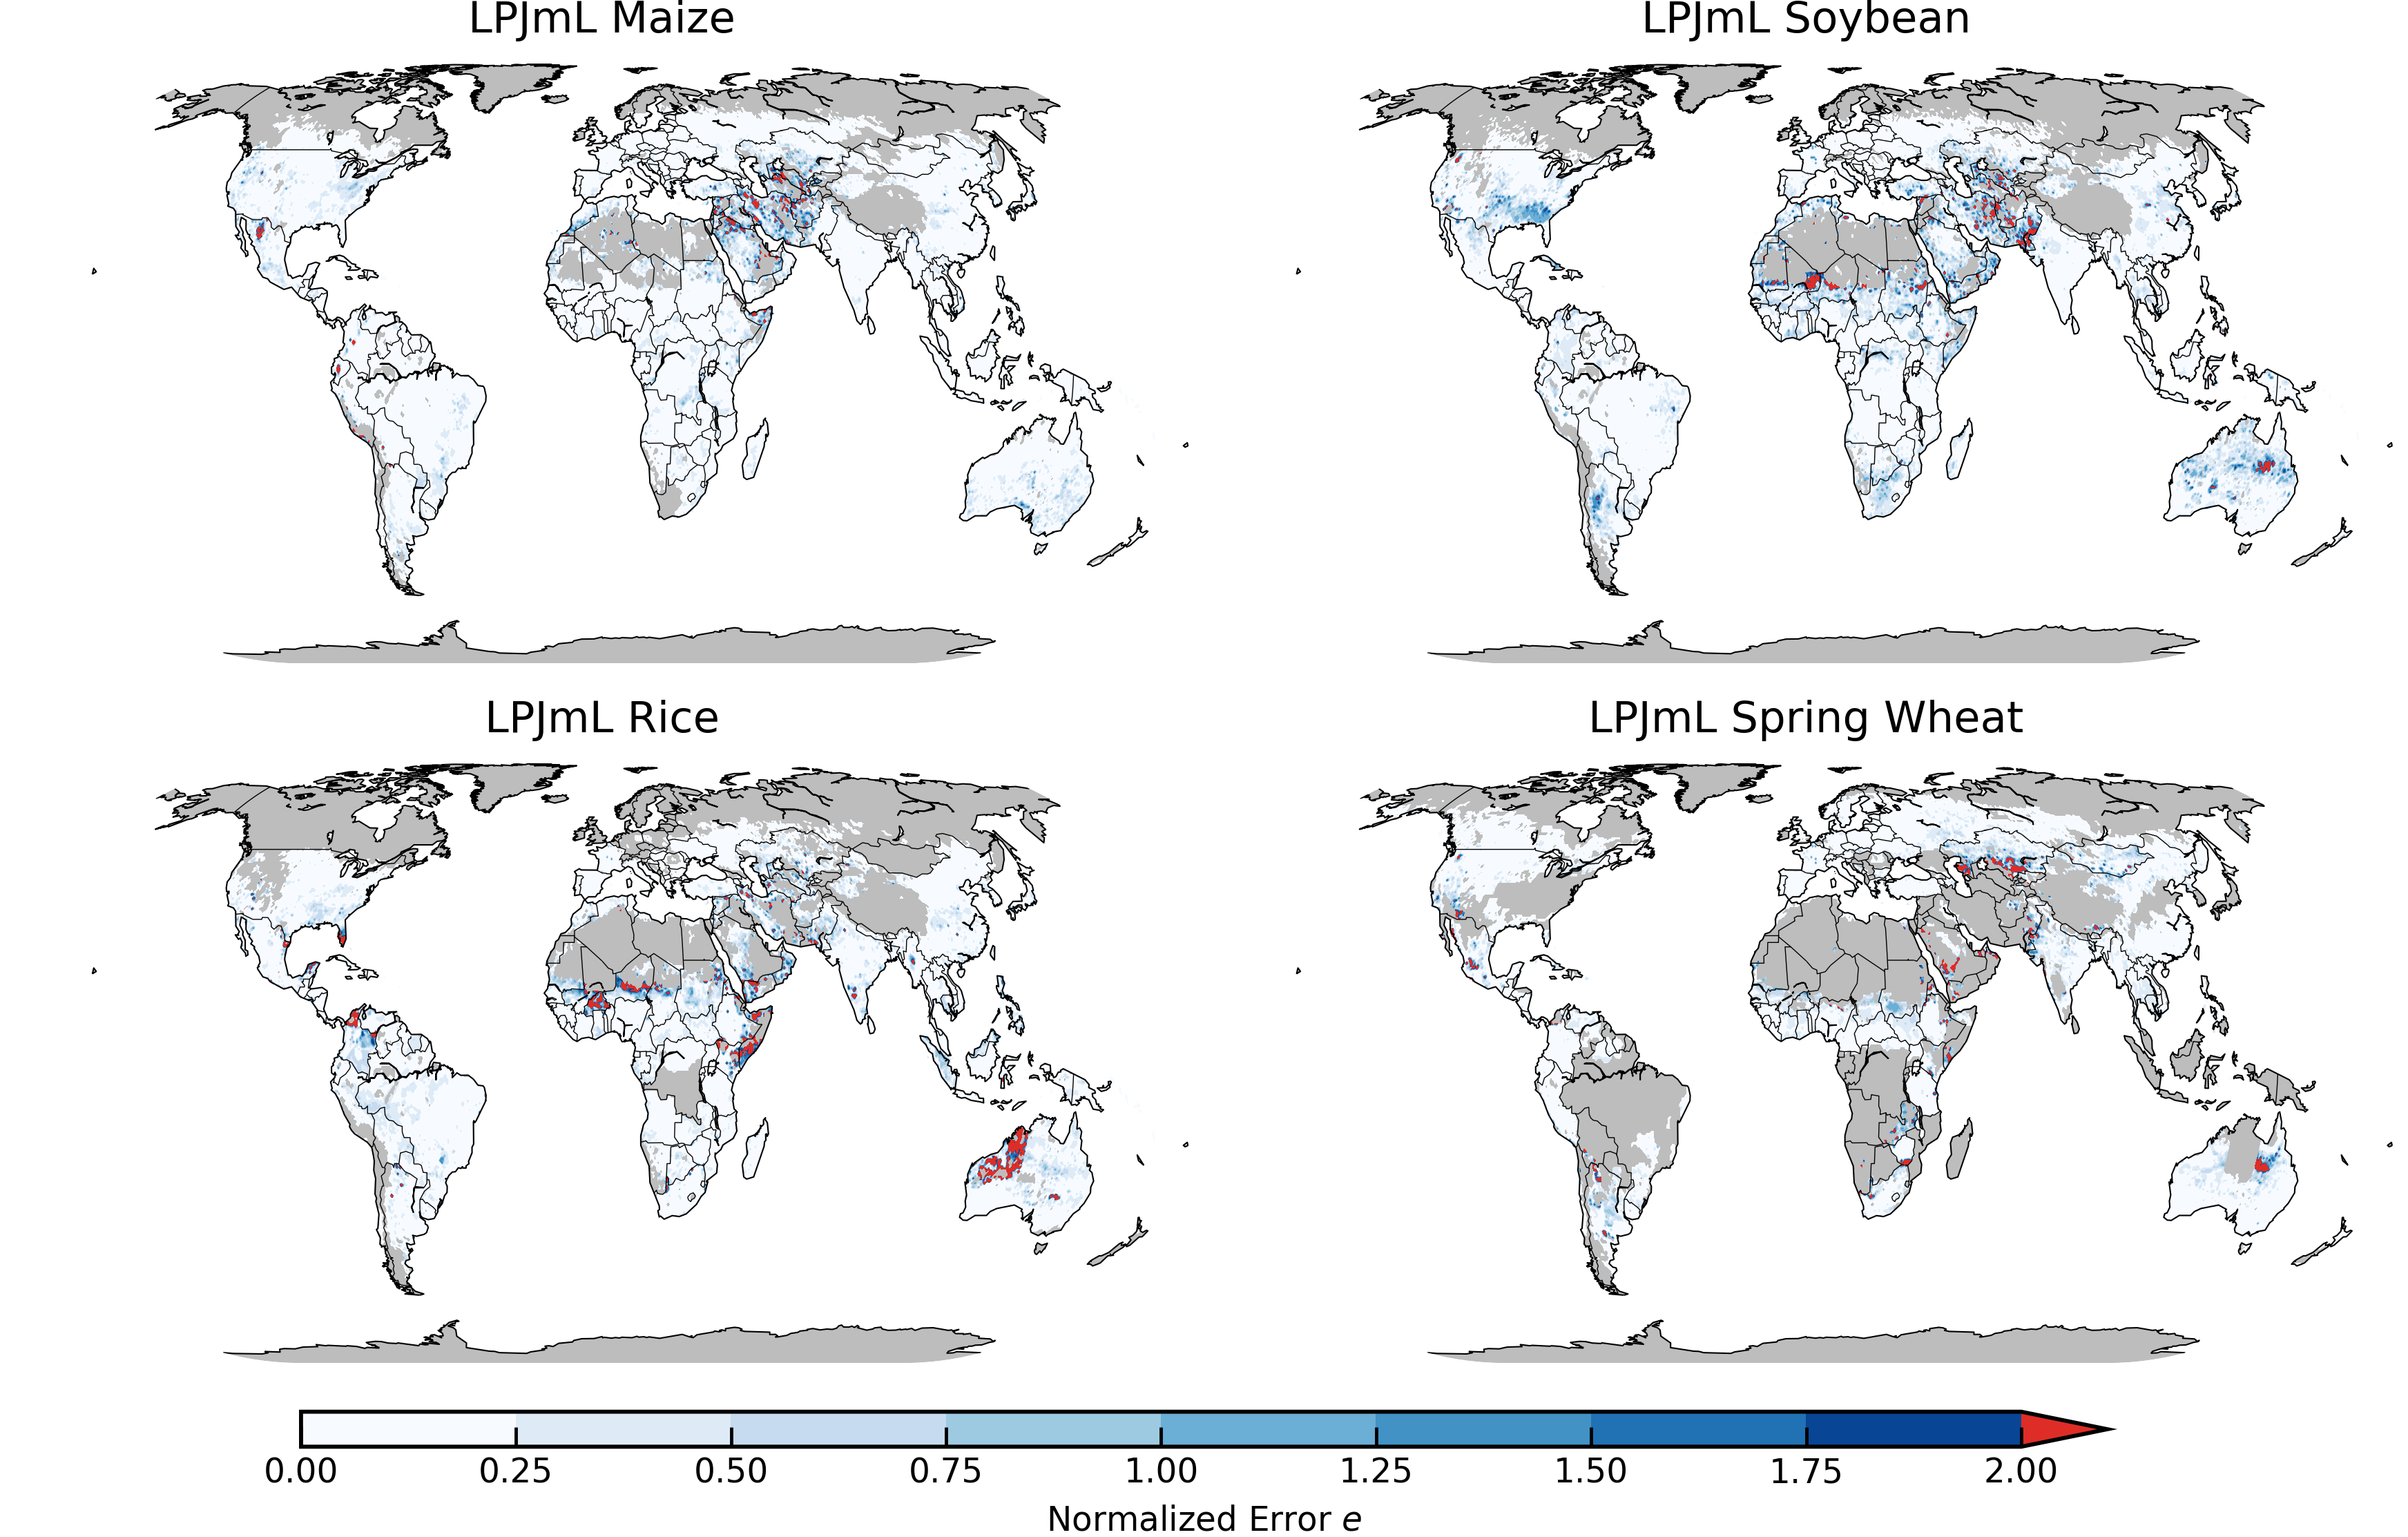
\includegraphics[width=15.5cm]{LPJmL_spatial_error.png}
  \caption{Normalized error $e$ for LPJmL. Same convention as main text Figure 8.}
\end{figure}

\begin{figure}[h!]
  \centering
  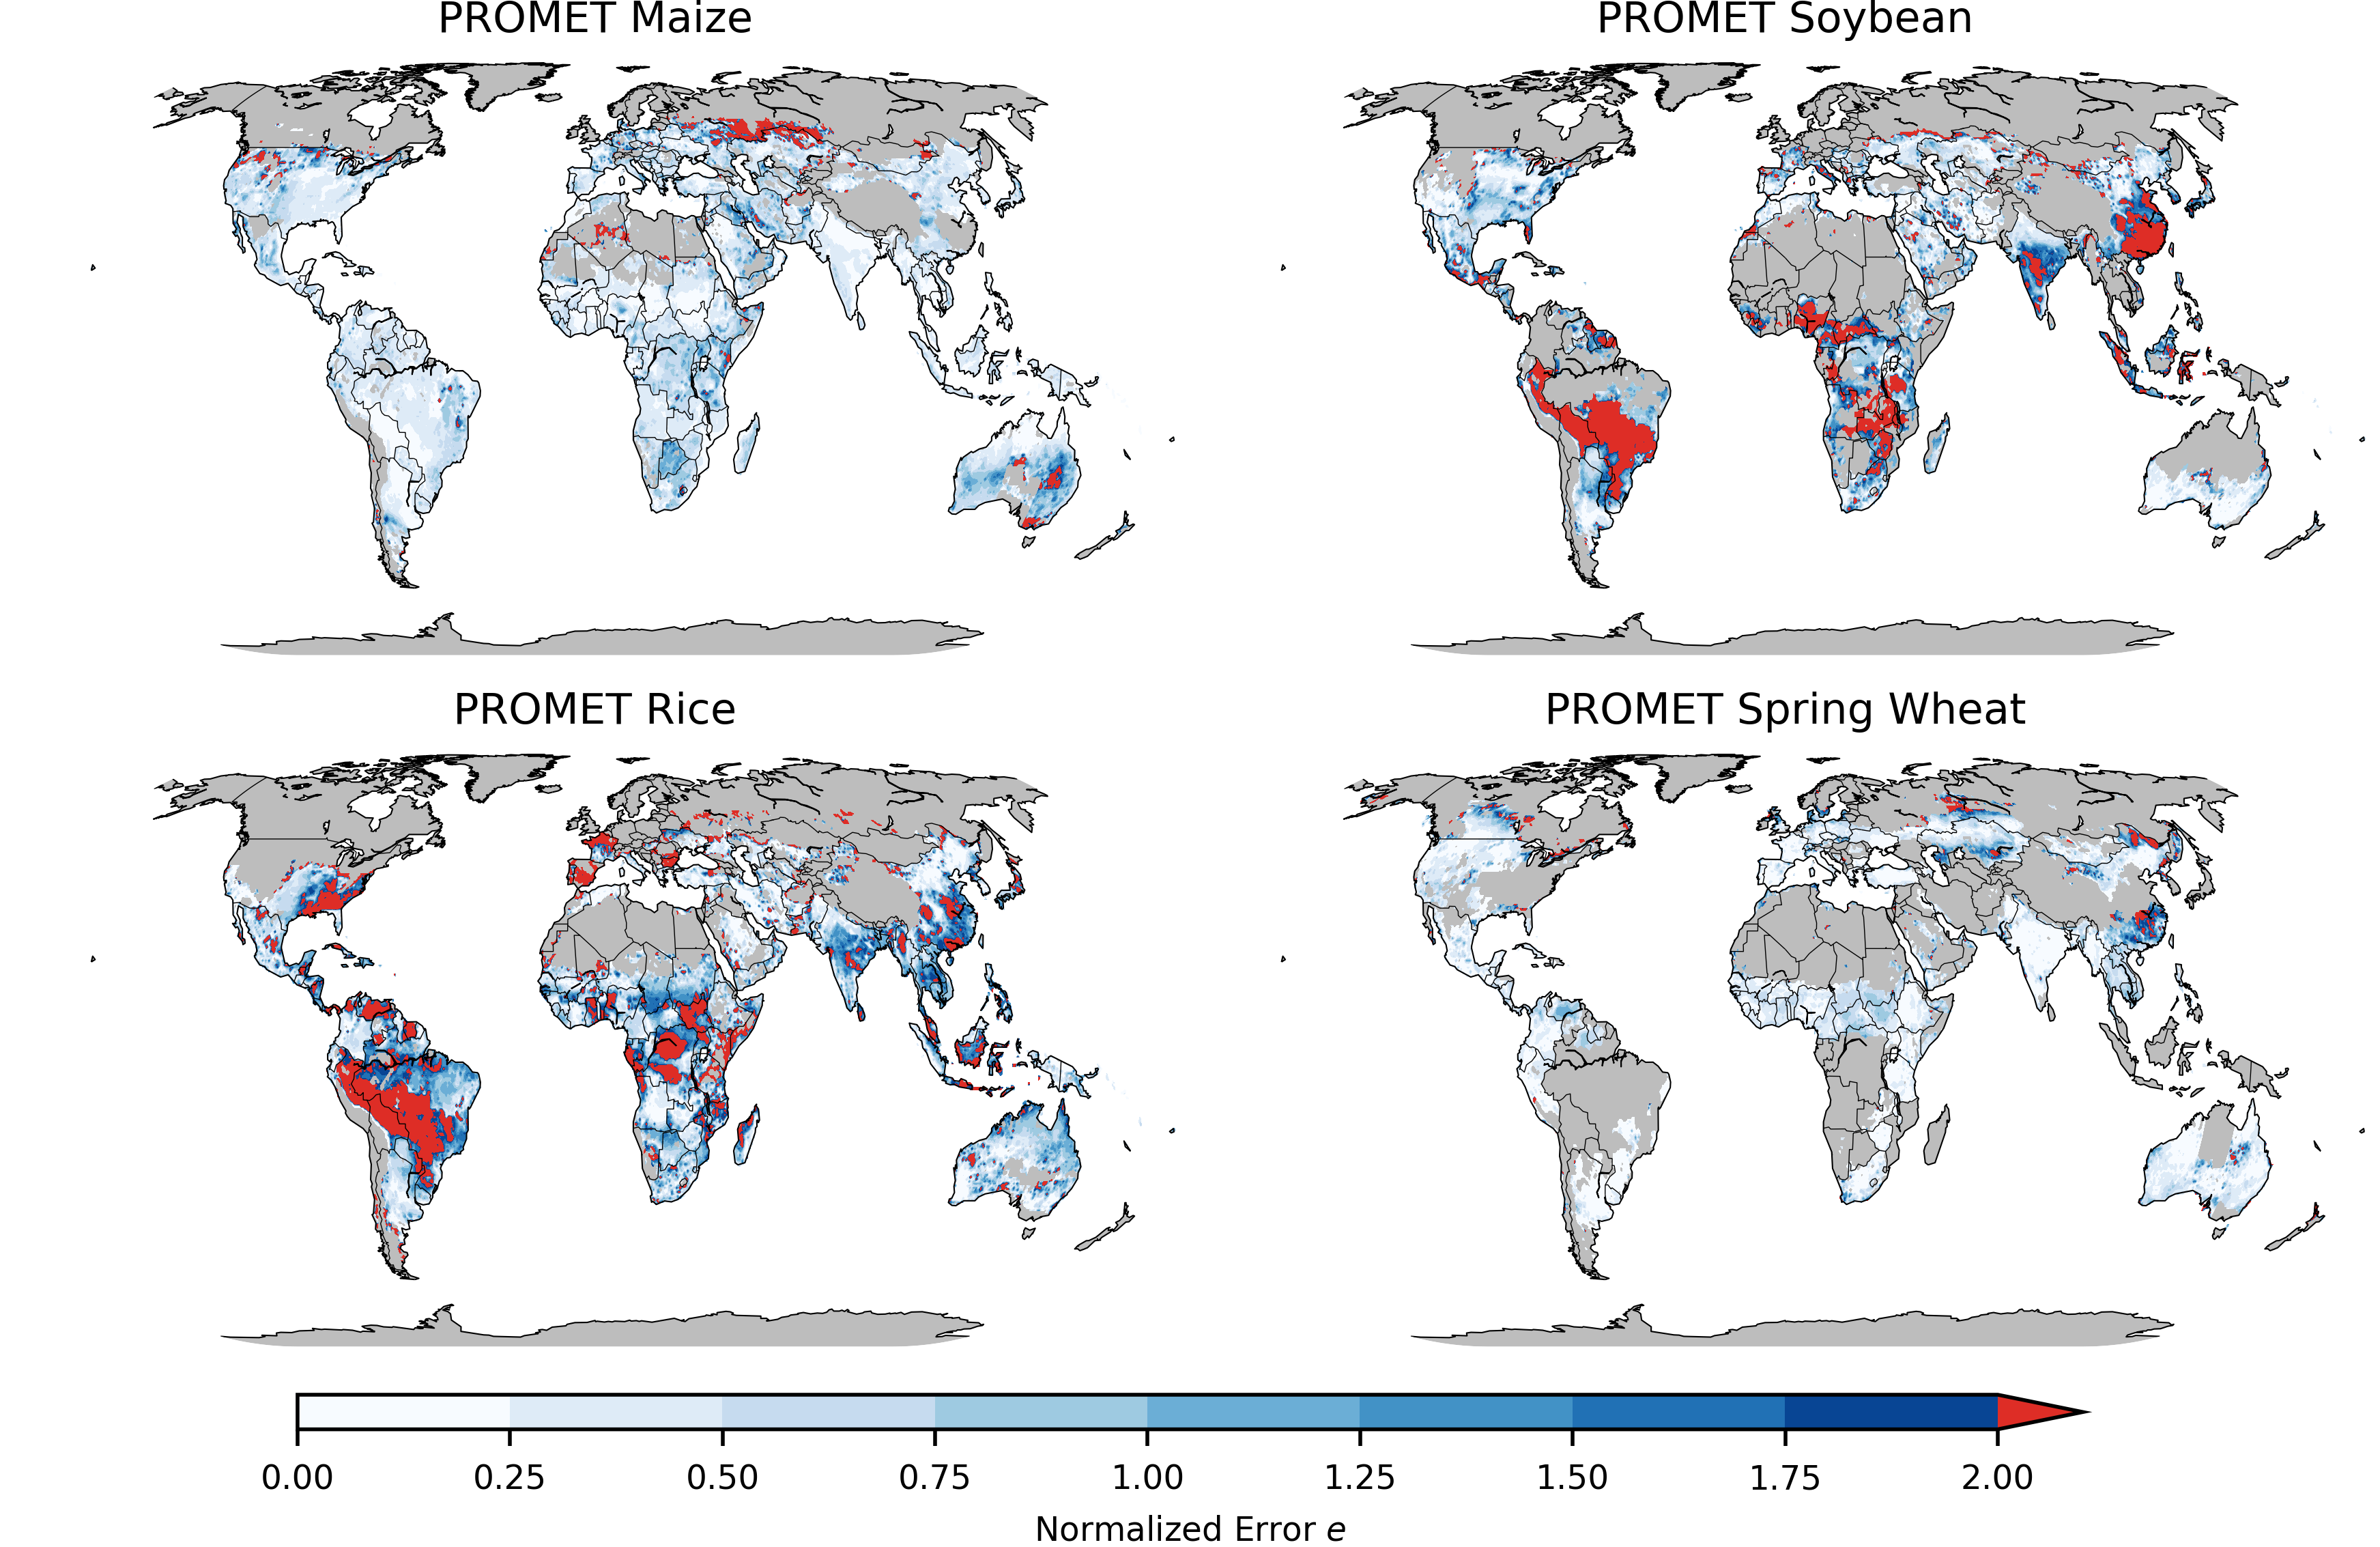
\includegraphics[width=15.5cm]{PROMET_spatial_error.png}
  \caption{Normalized error $e$ for PROMET. Same convention as main text Figure 8.}
\end{figure}

\begin{figure}[h!]
  \centering
  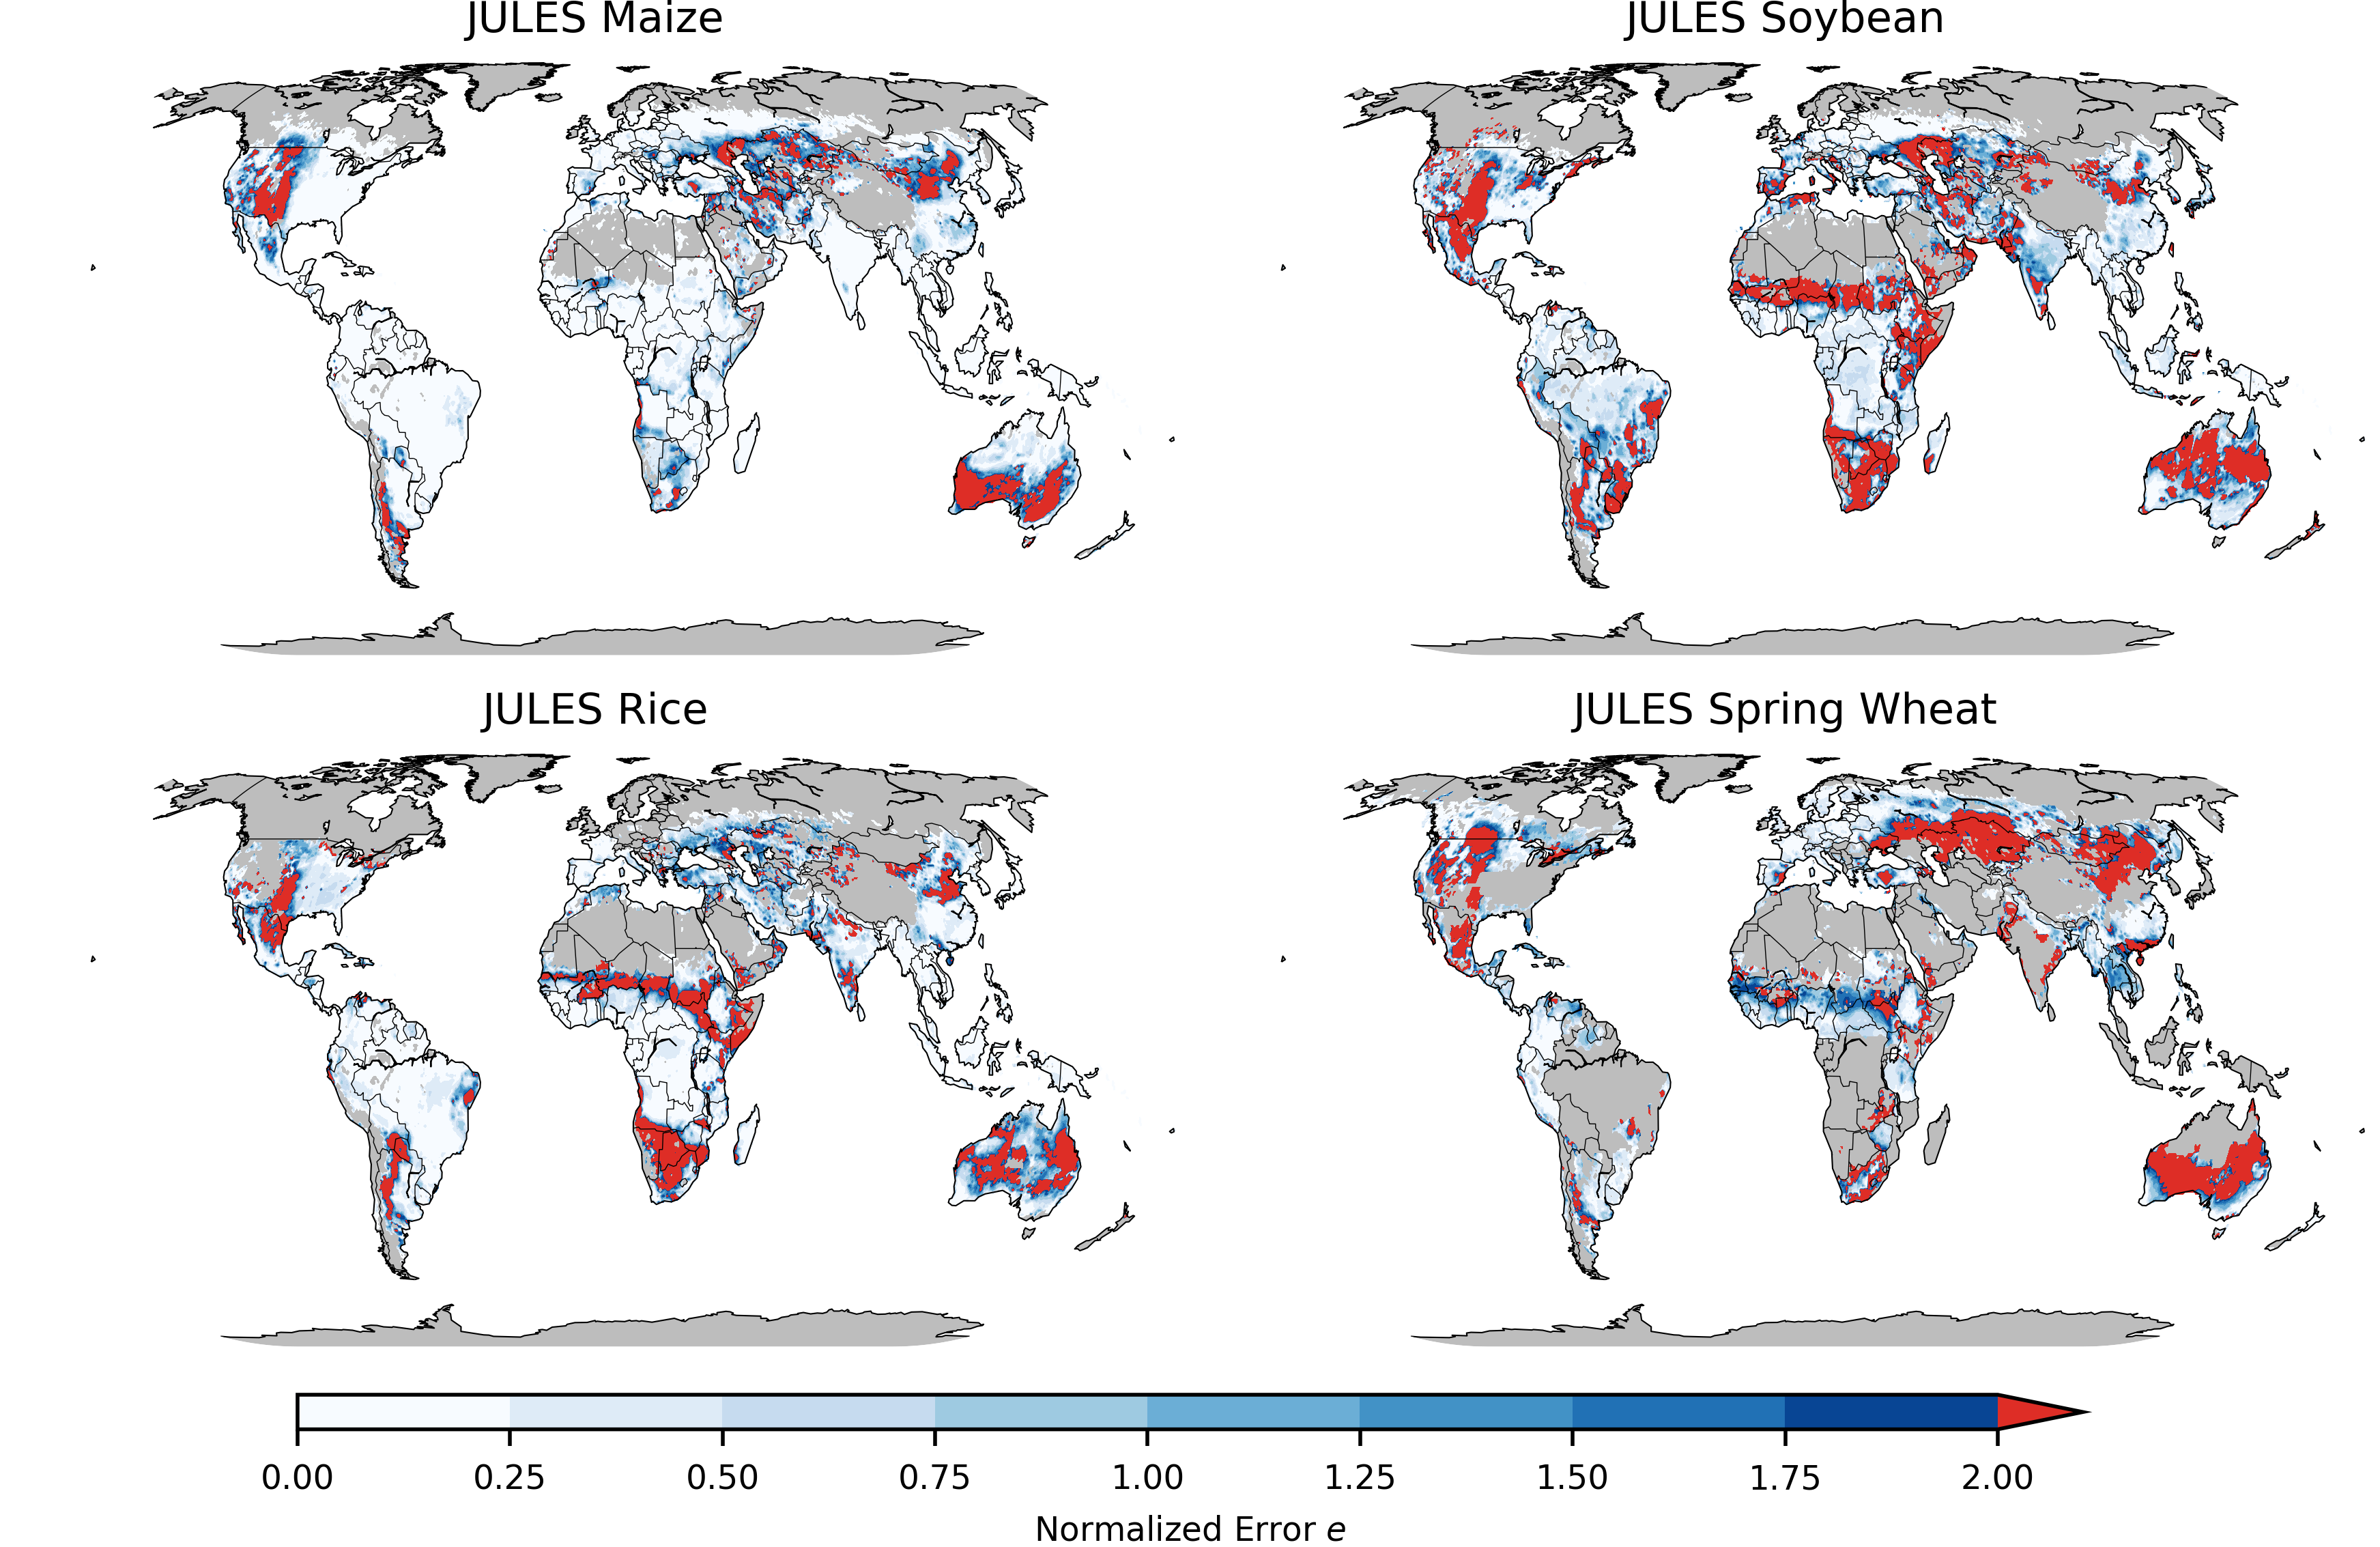
\includegraphics[width=15.5cm]{JULES_spatial_error.png}
  \caption{Normalized error $e$ for JULES. Same convention as main text Figure 8.}
\end{figure}

\begin{figure}[h!]
  \centering
  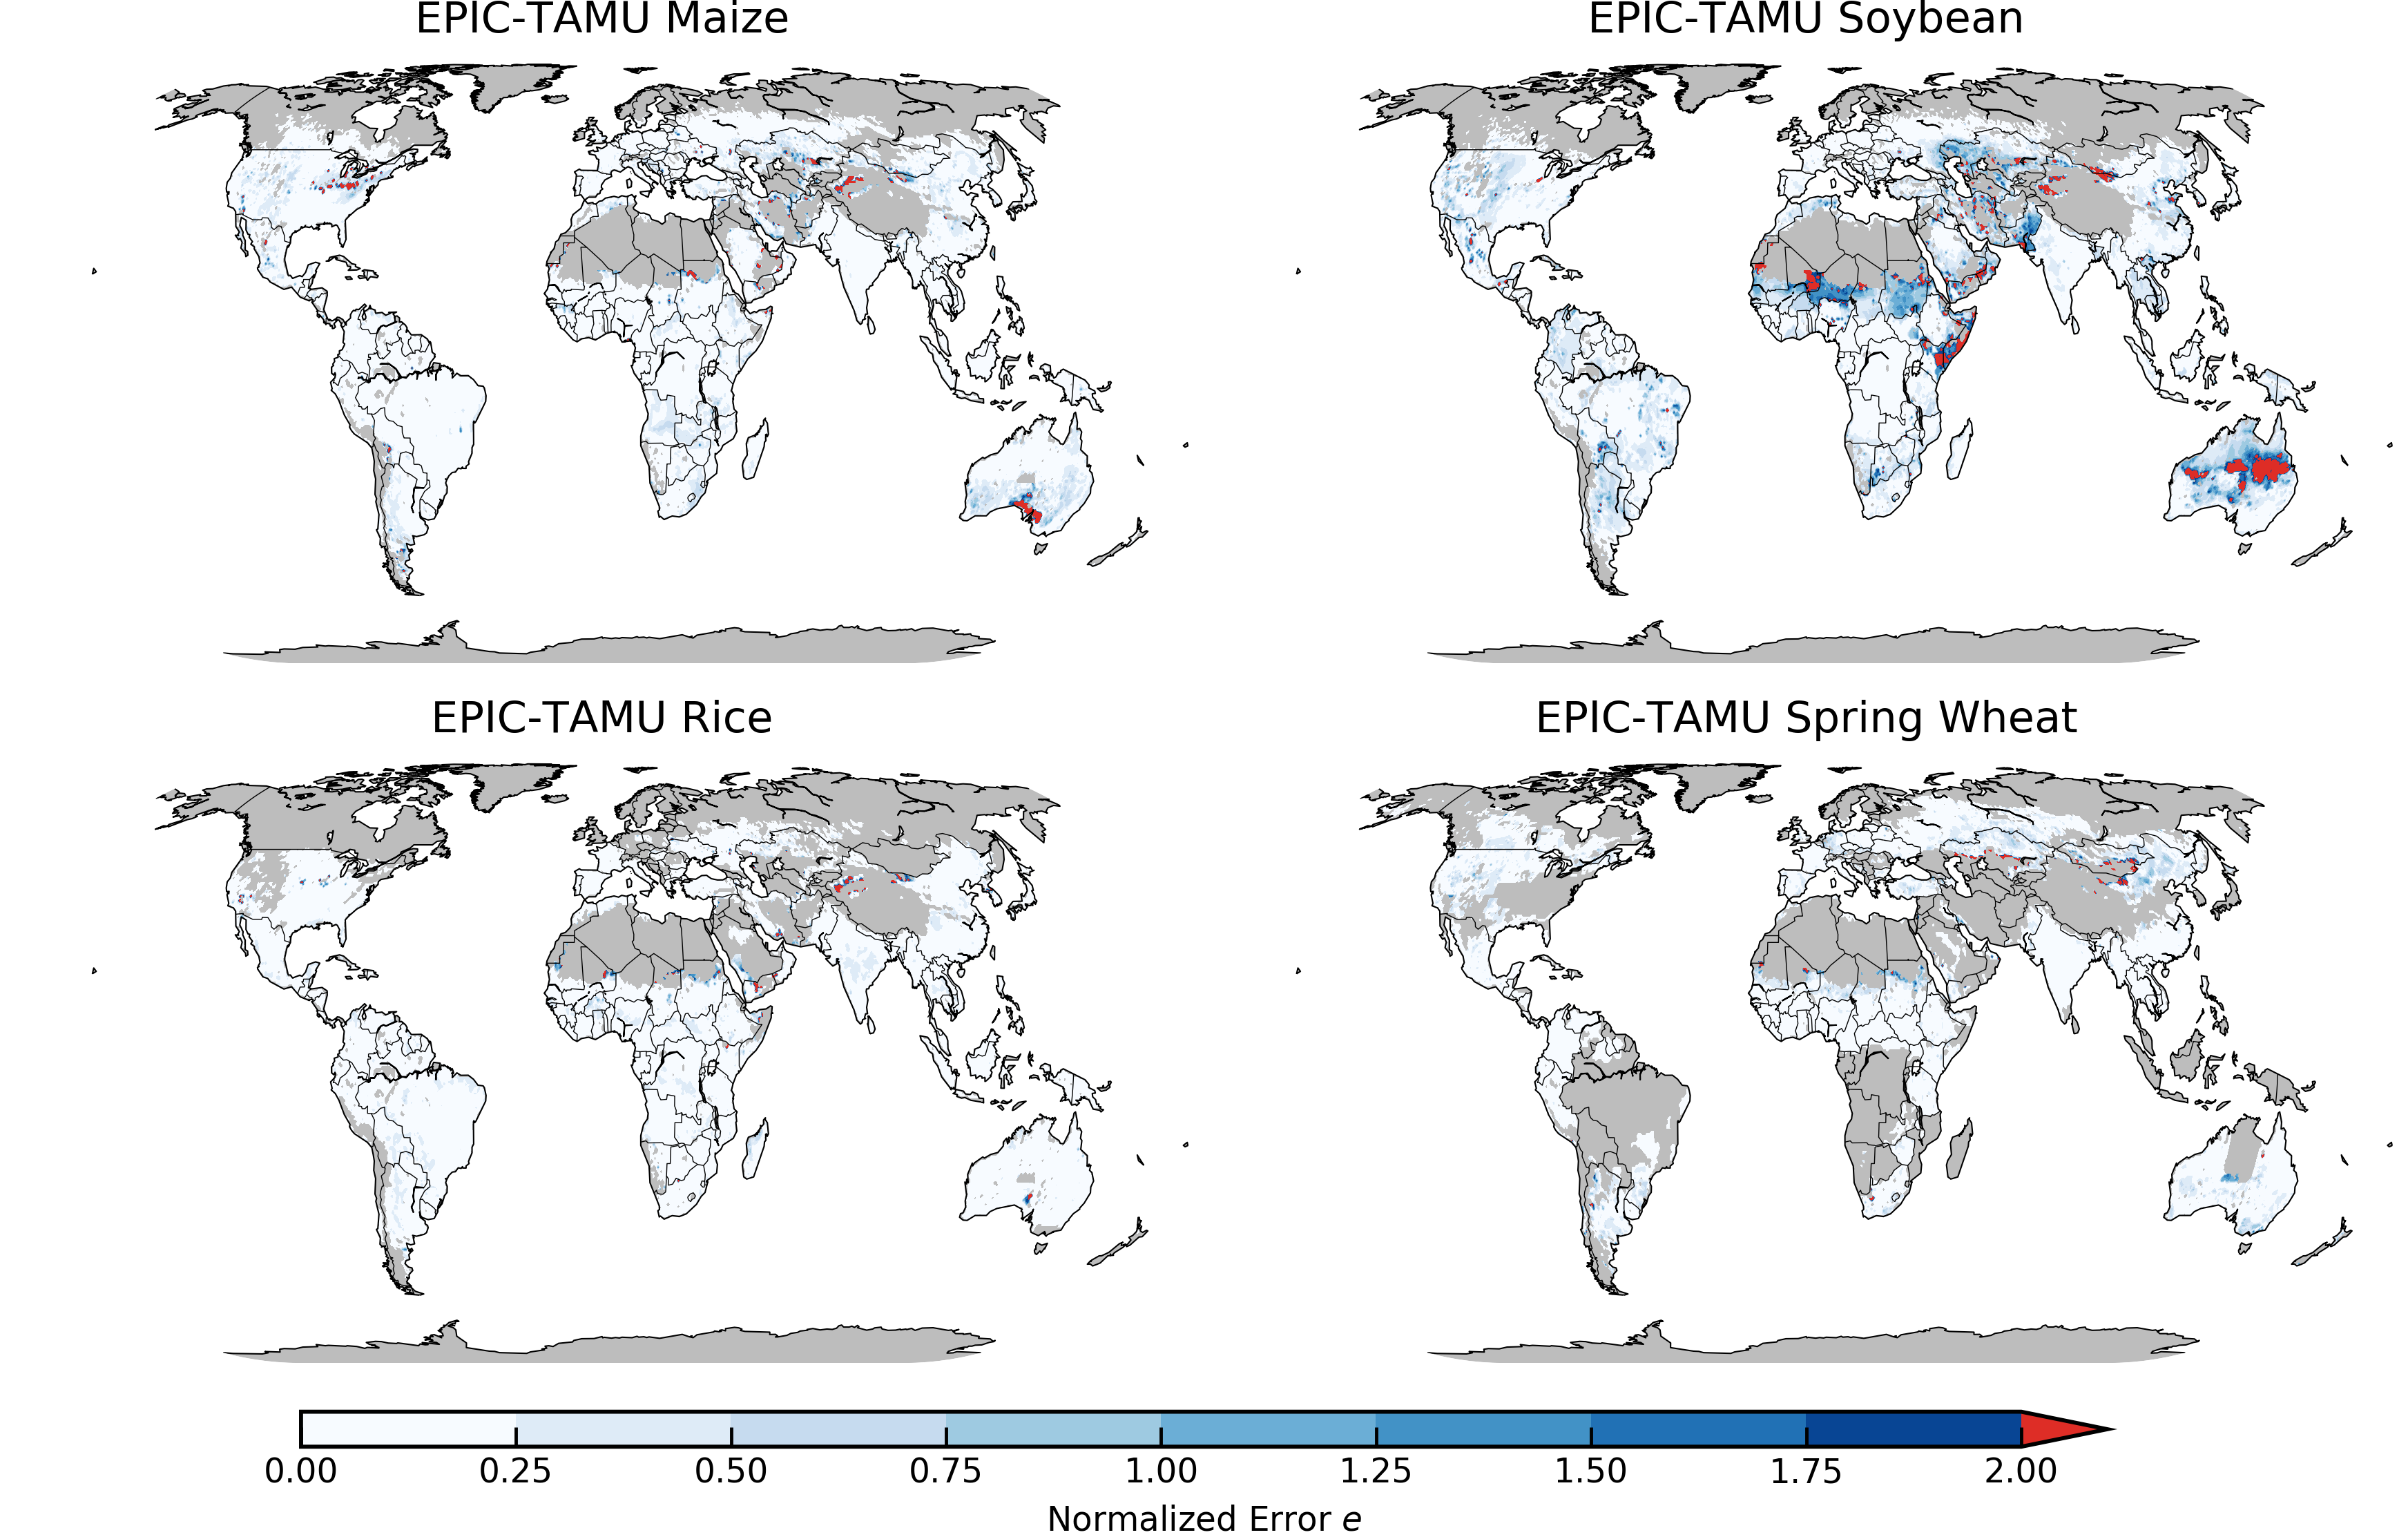
\includegraphics[width=15.5cm]{EPIC-TAMU_spatial_error.png}
  \caption{Normalized error $e$ for EPIC-TAMU. Same convention as main text Figure 8.}
\end{figure}

\begin{figure}[h!]
  \centering
  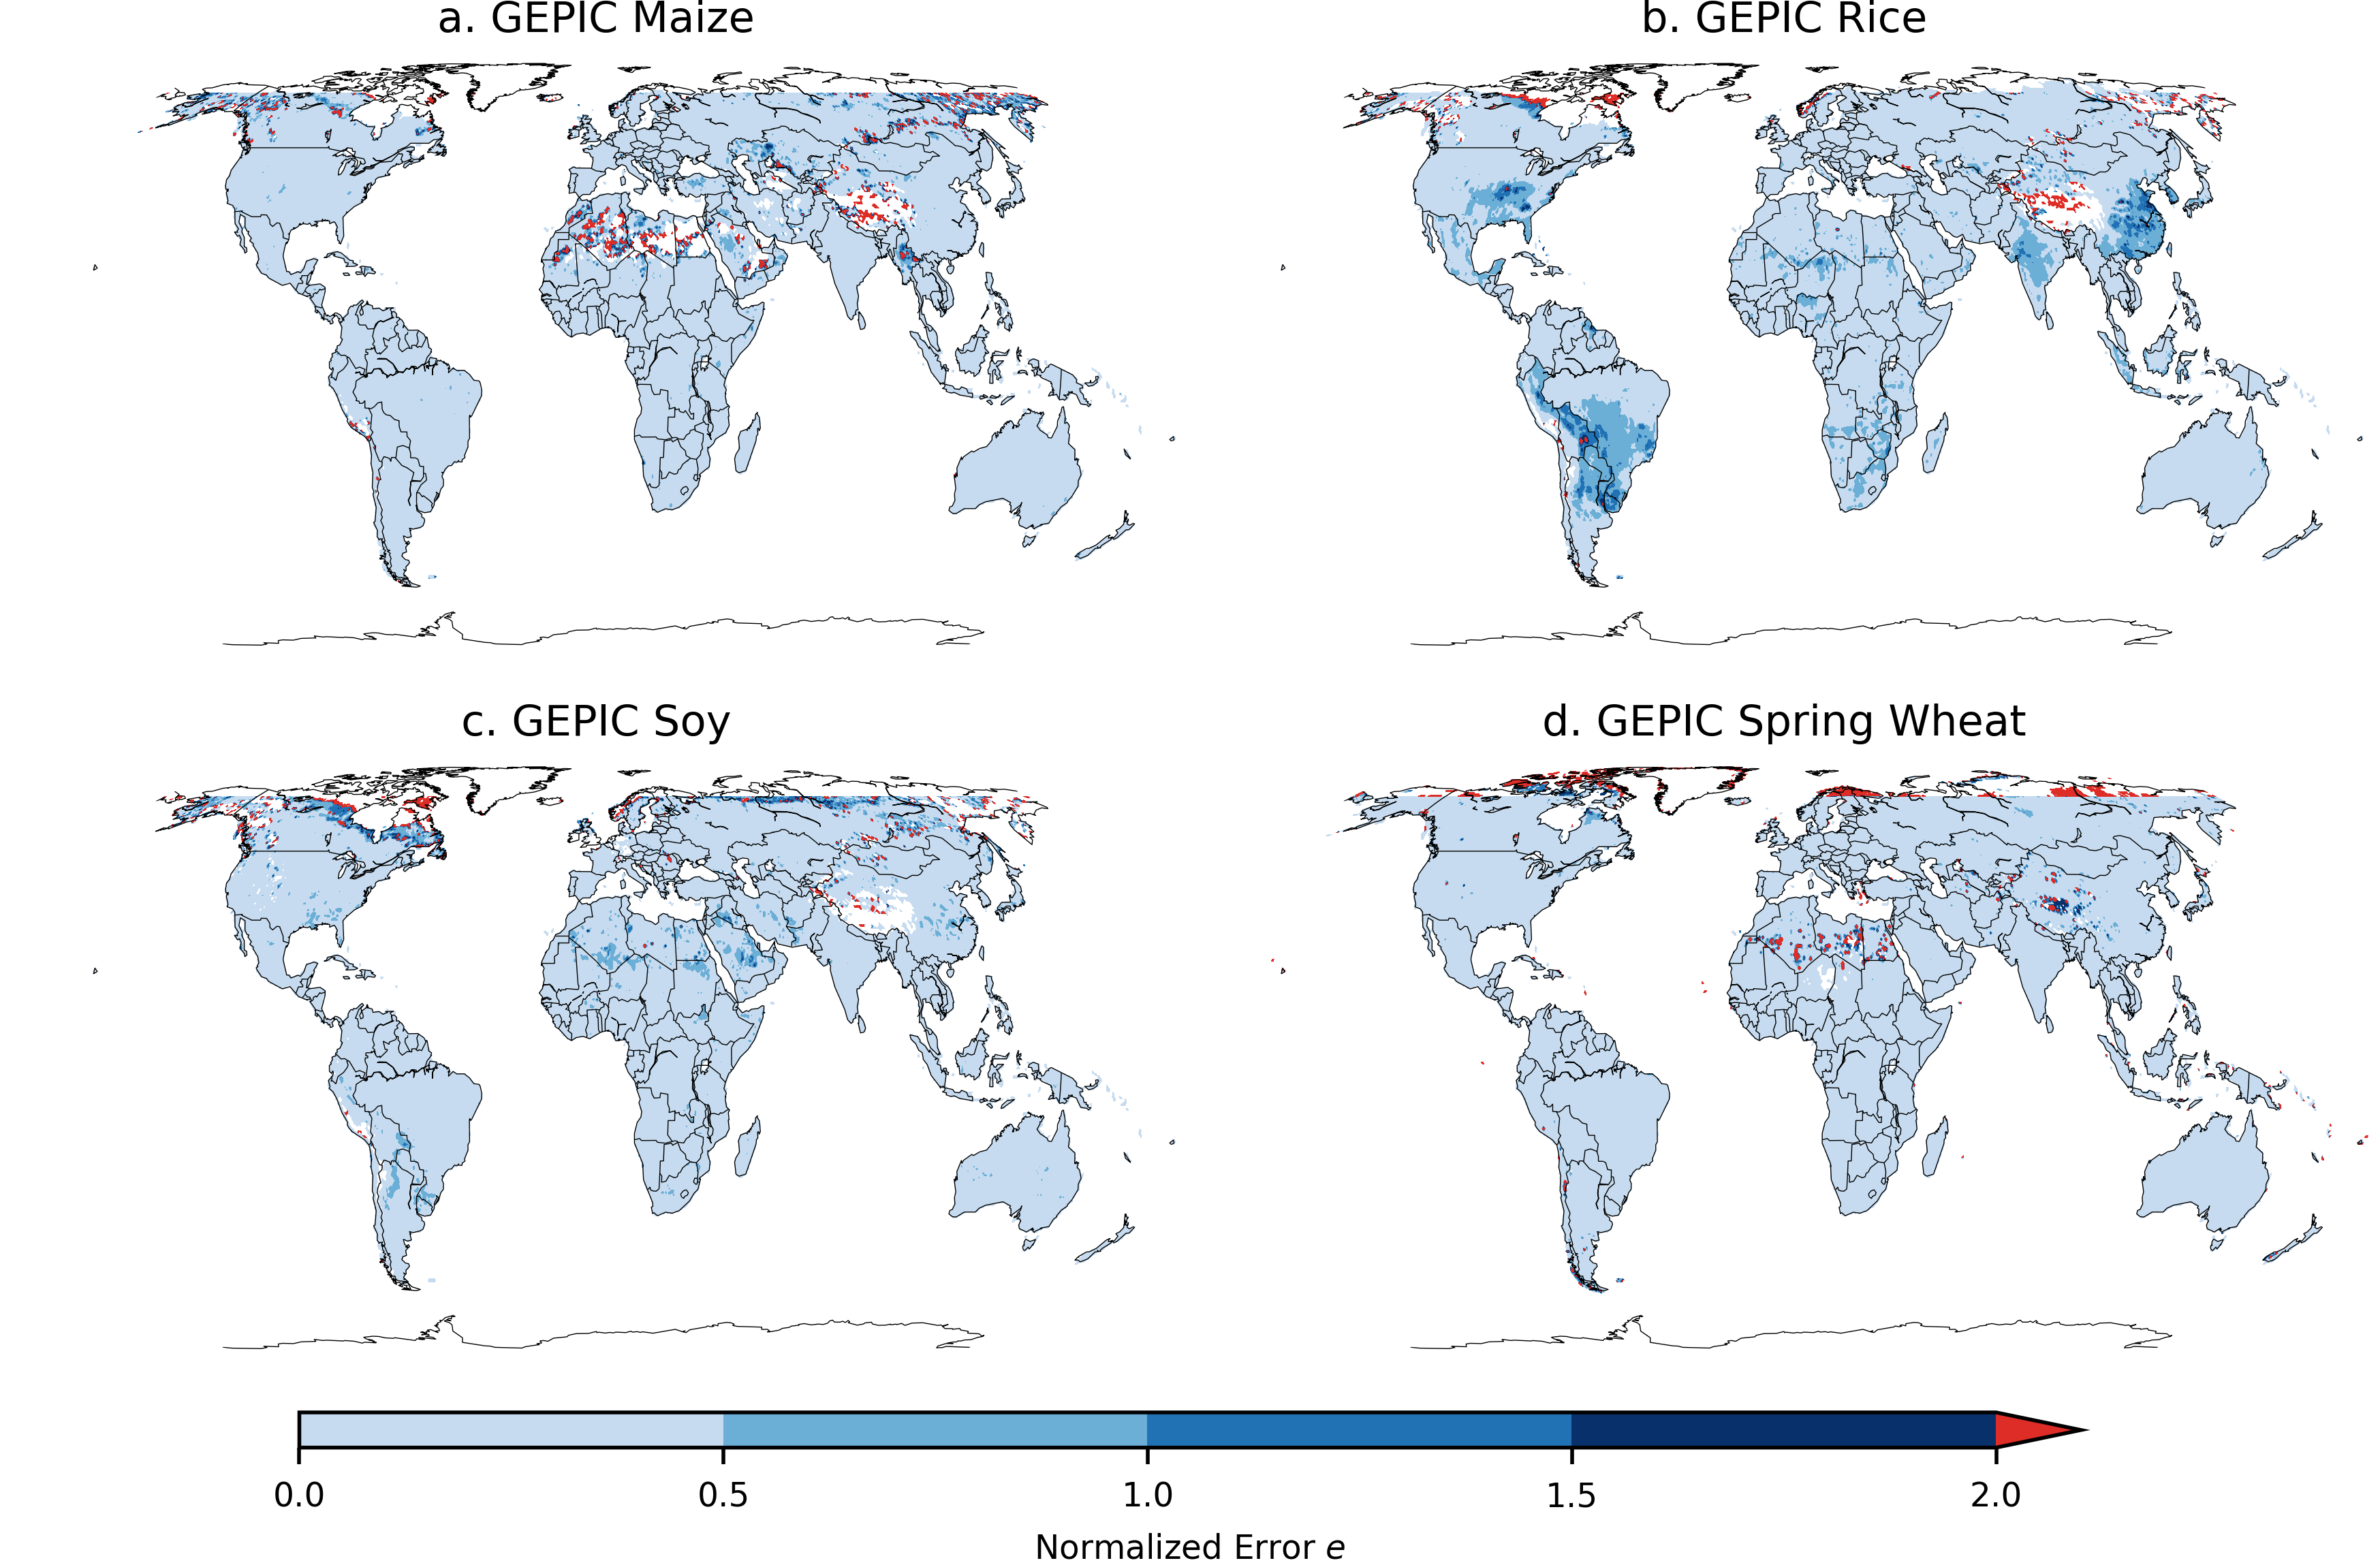
\includegraphics[width=15.5cm]{GEPIC_spatial_error.png}
  \caption{Normalized error $e$ for GEPIC. Same convention as main text Figure 8.}
\end{figure}

\begin{figure}[h!]
  \centering
  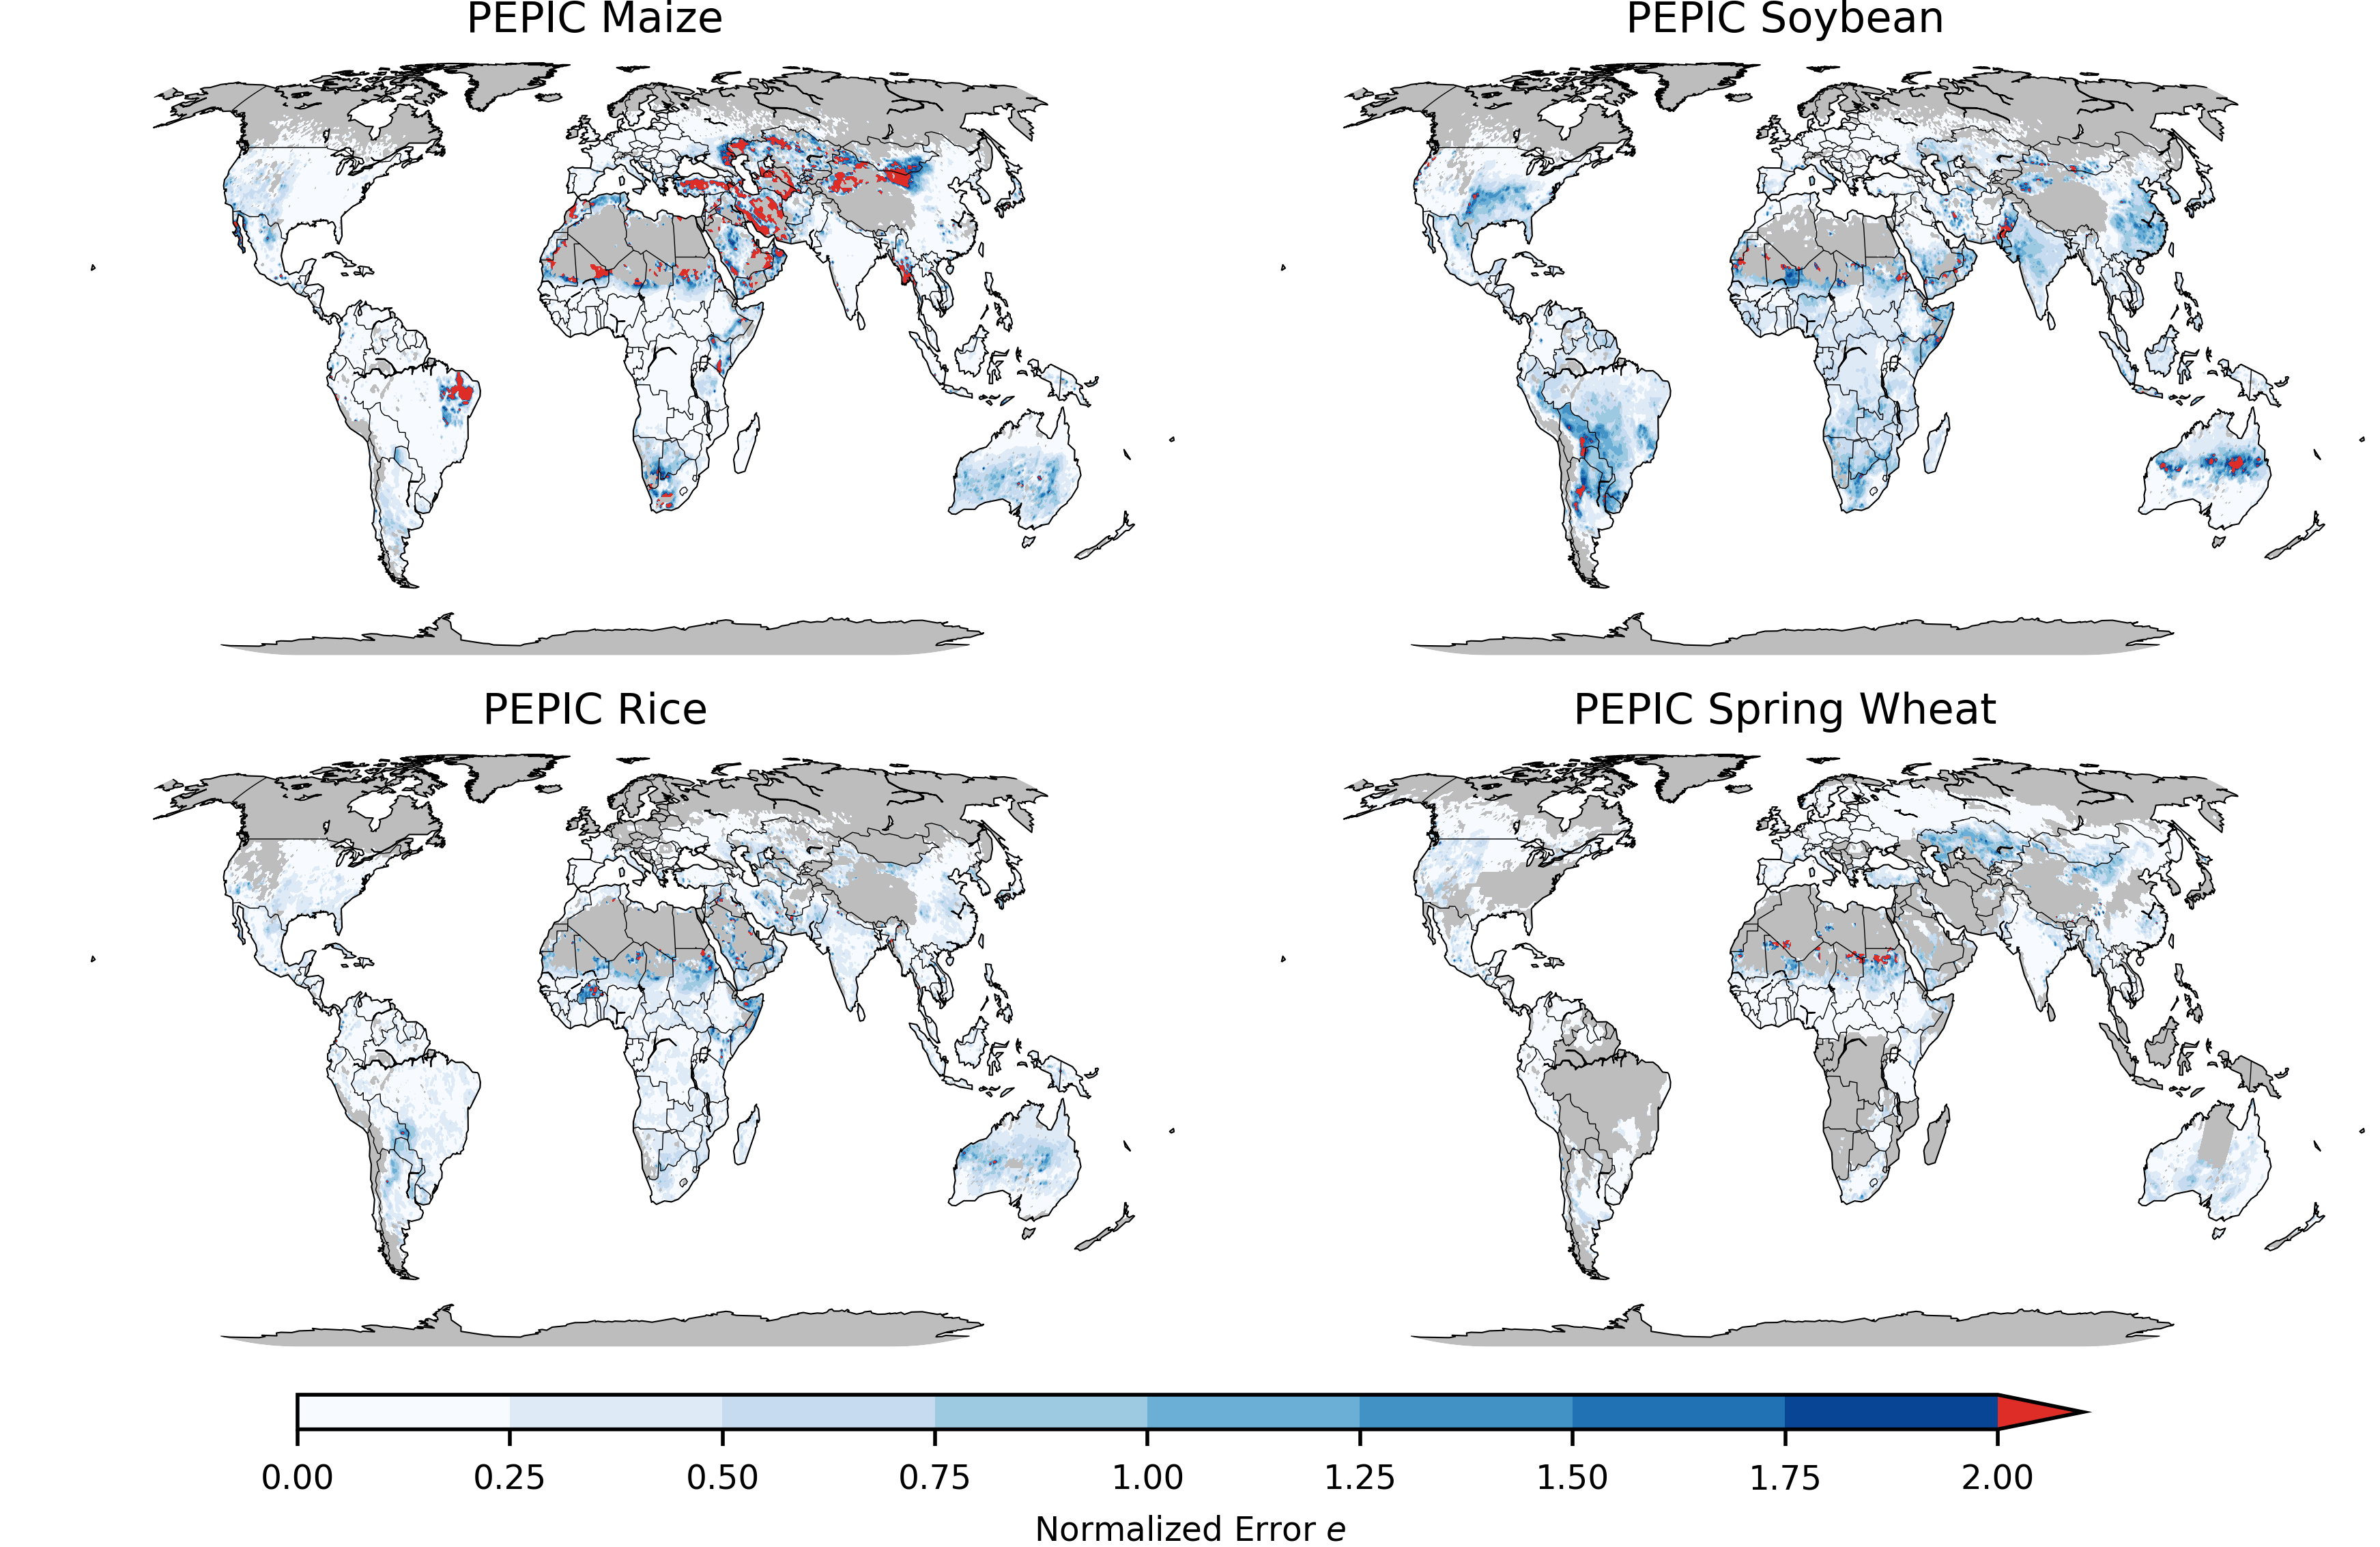
\includegraphics[width=15.5cm]{PEPIC_spatial_error.png}
  \caption{Normalized error $e$ for PEPIC. Same convention as main text Figure 8.}
\end{figure}

%%%%%%%%%%%%%%%%%%%%%%%%%%%%%%%%%%%%%%%%%%%%%%%%%%%%%%%%%%%%%%%%%%%%%%%%%%%%%%%%%%%%%%%
%%%%%%%%%%%%%%%%%%%%%%%%%%%%%%%%%%%%%%%%%%%%%%%%%%%%%%%%%%%%%%%%%%%%%%%%%%%%%%%%%%%%%%%
%%%%%%%%%%%%%%%%%%%%%%%%%%%%%%%%%%%%%%%%%%%%%%%%%%%%%%%%%%%%%%%%%%%%%%%%%%%%%%%%%%%%%%%
\clearpage
\section{Cross validation error for all models}

\begin{figure}[h!]
  \centering
  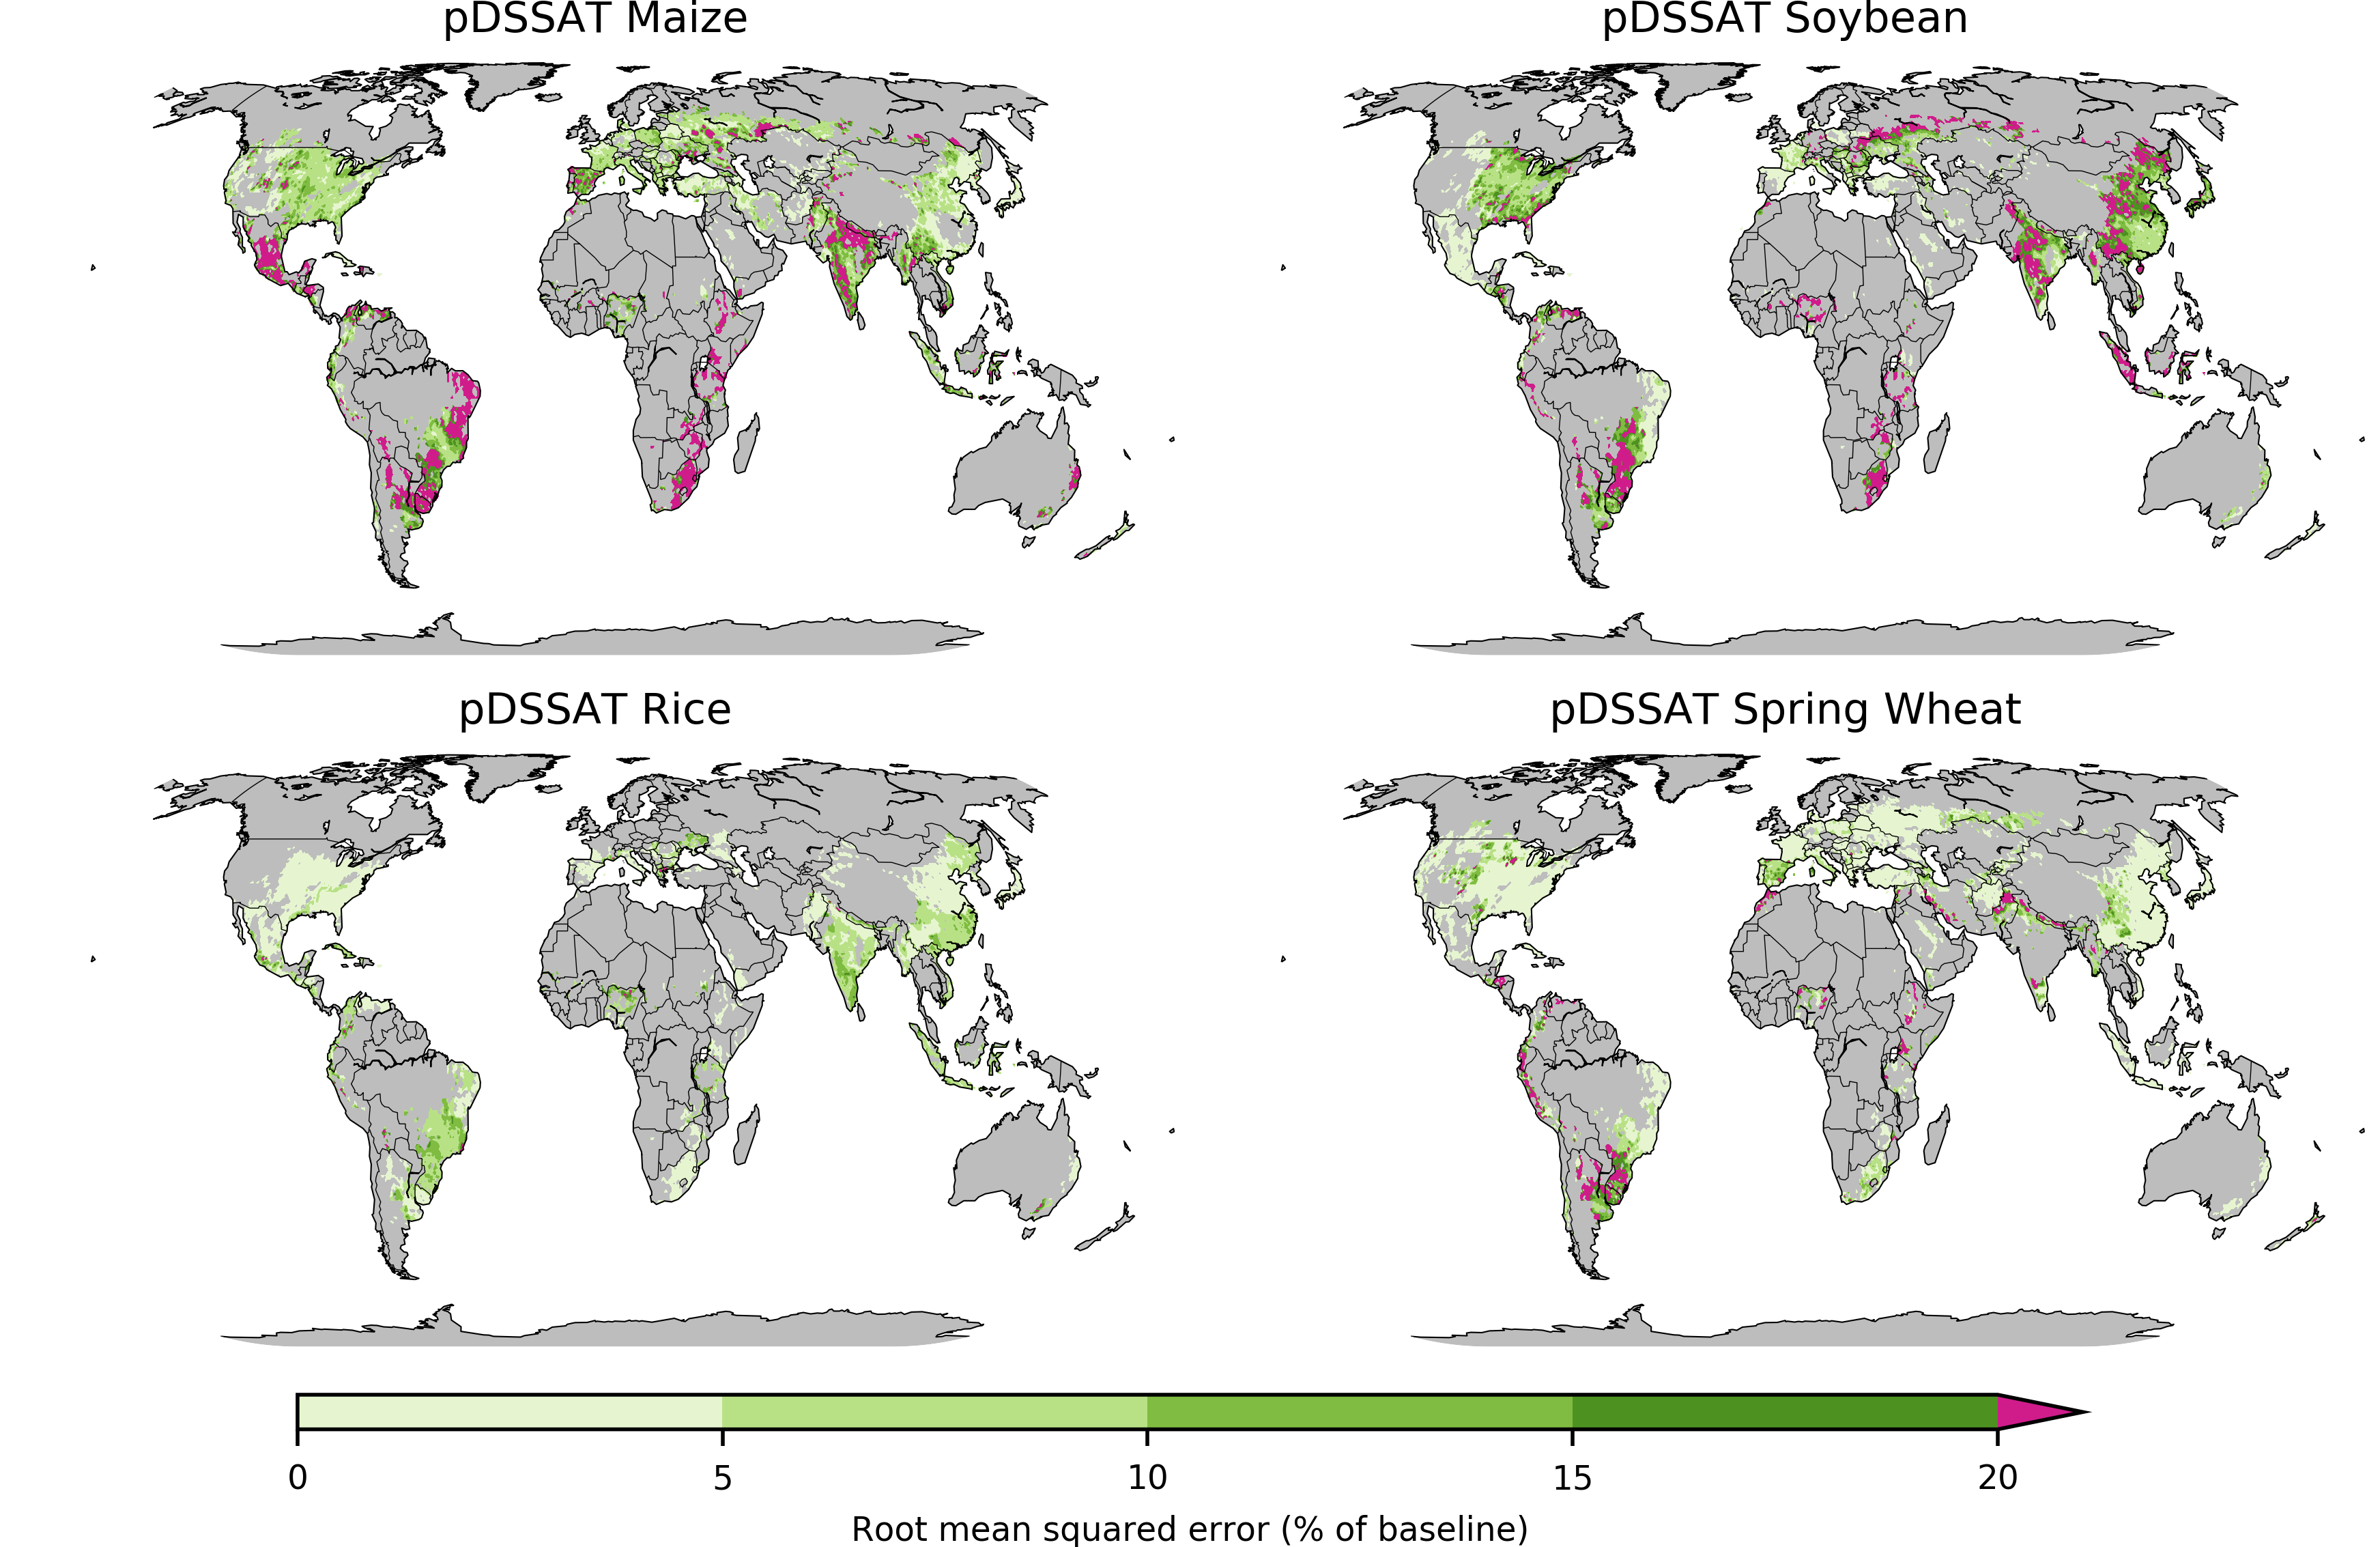
\includegraphics[width=15.5cm]{pDSSAT_spatial_MSE_ton_ha.png}
  \caption{Root mean squared error for three-fold cross validation for the pDSSAT model for rainfed crops. Values shown as a percentage of baseline yield in each gridcell.}
\end{figure}

\begin{figure}[h!]
  \centering
  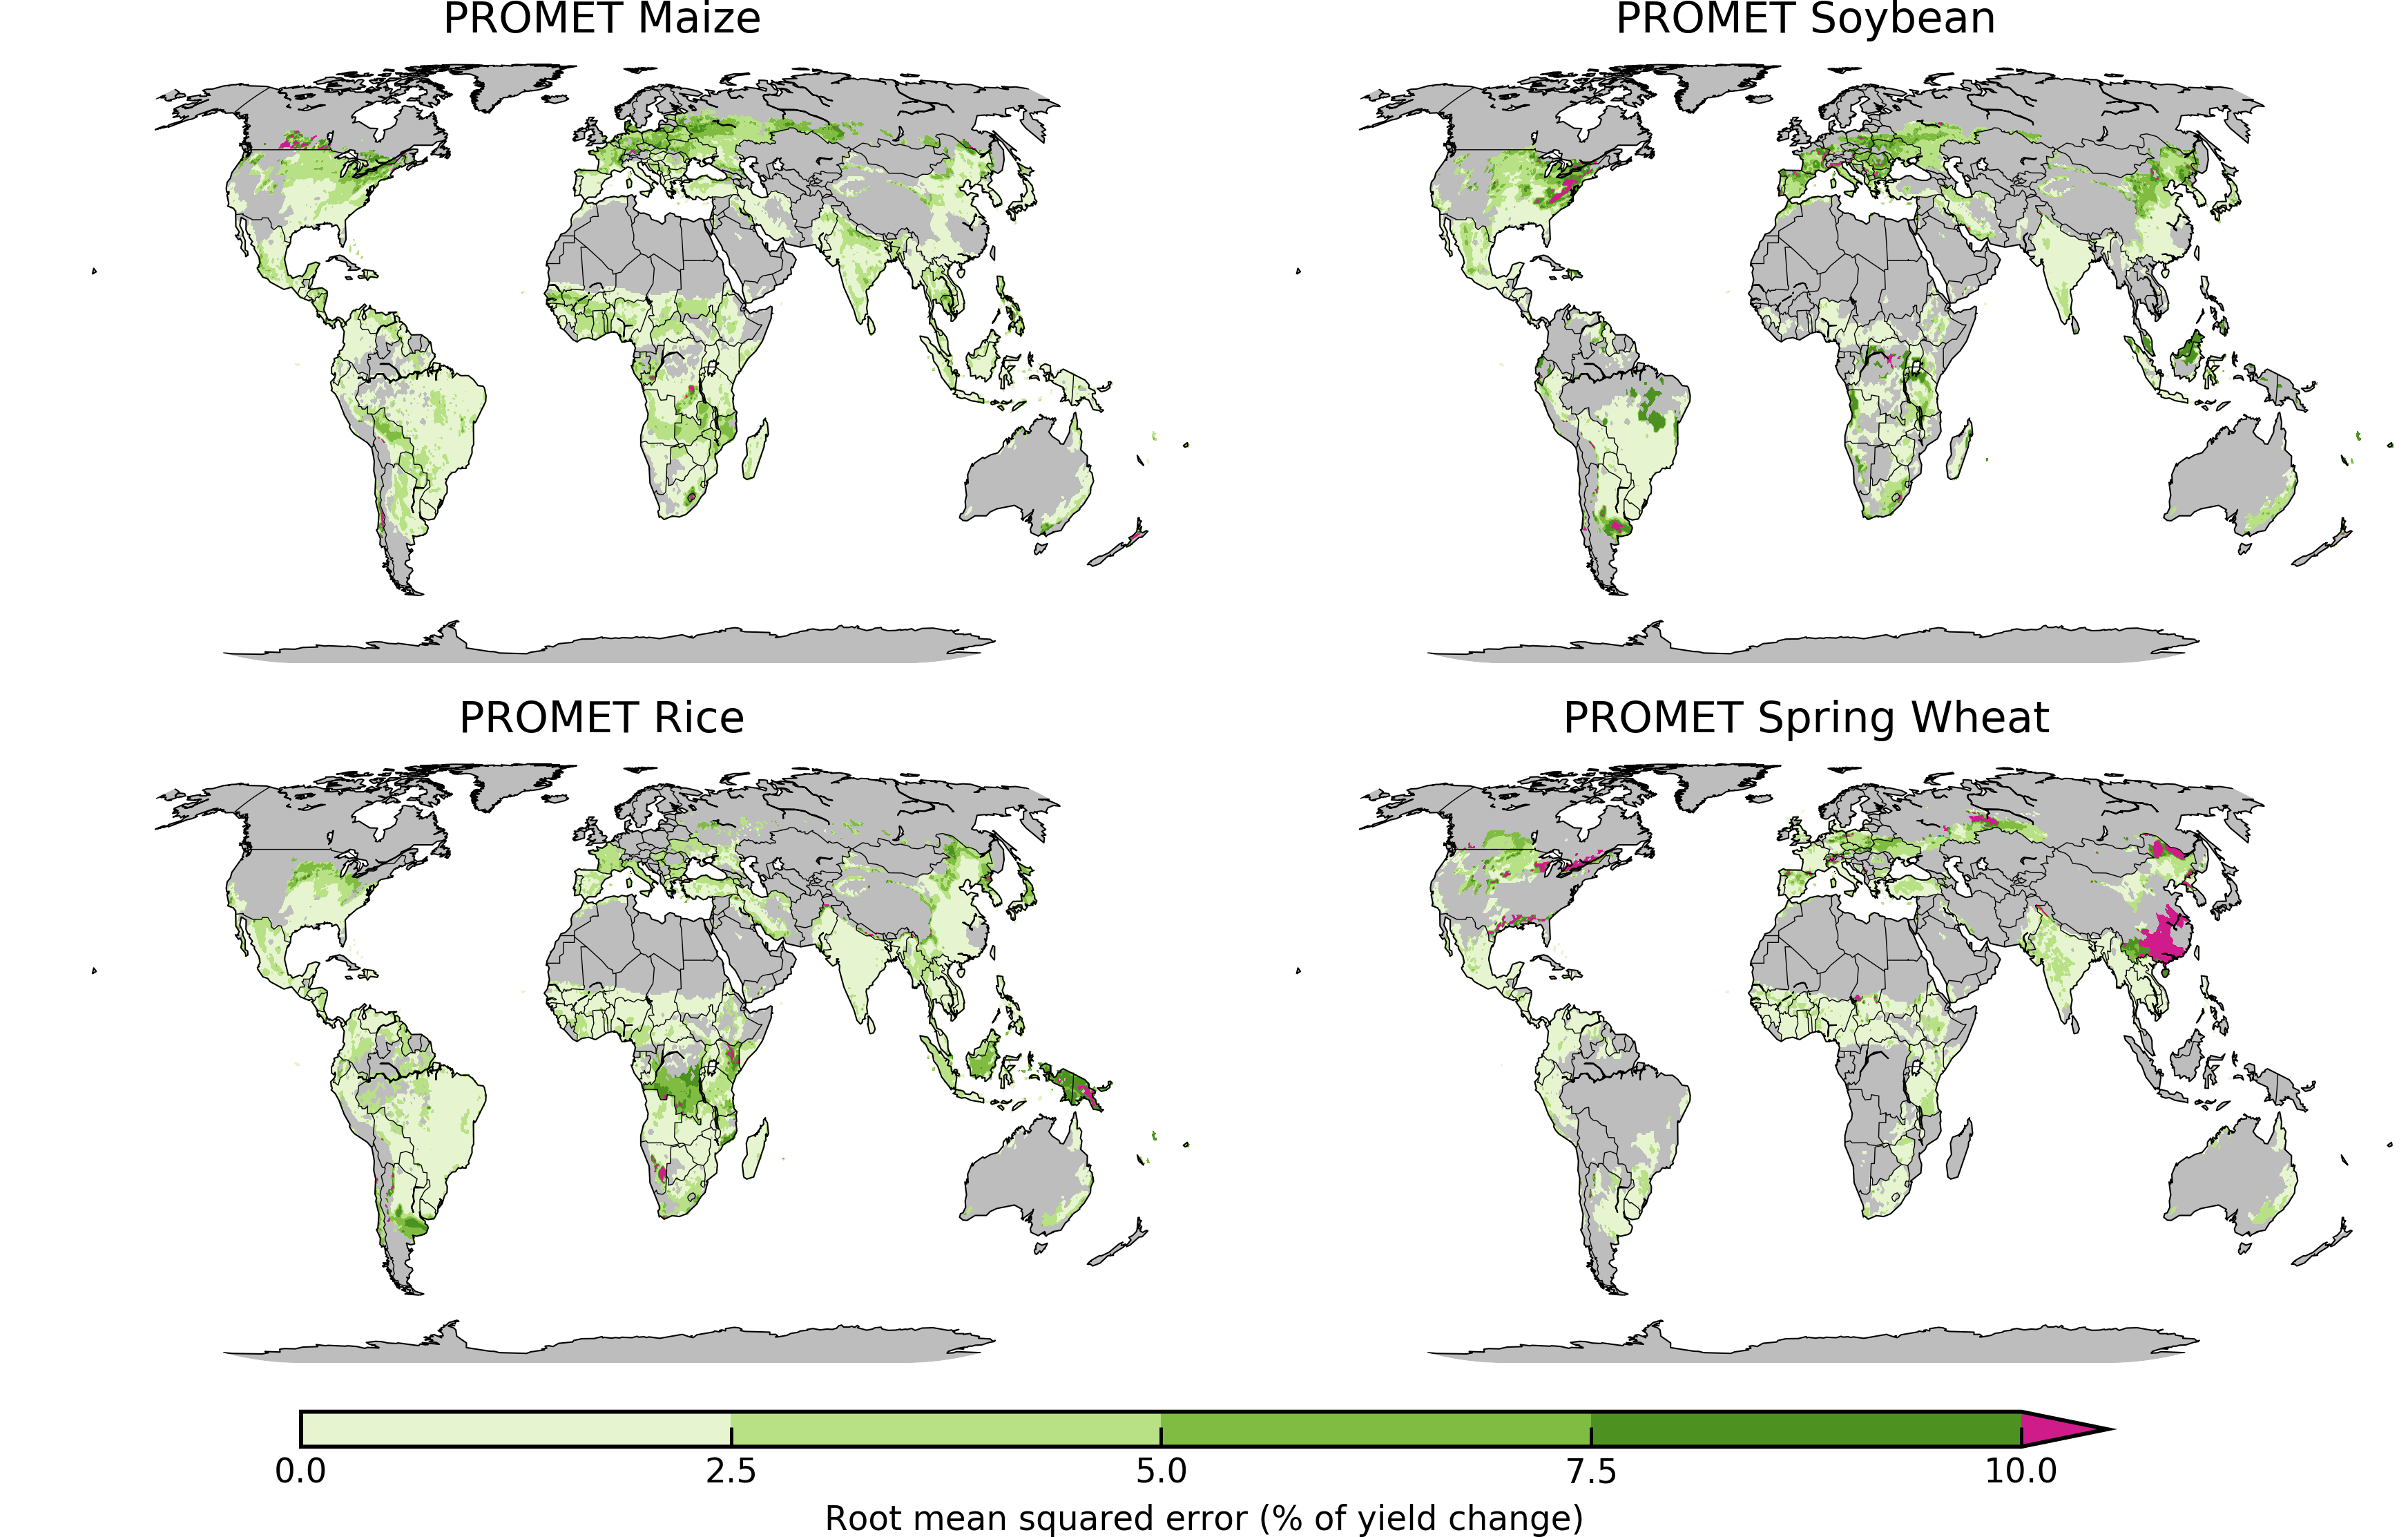
\includegraphics[width=15.5cm]{PROMET_spatial_MSE_ton_ha.png}
  \caption{Map of root mean squared error for three fold cross validation process for the PROMET model for rainfed crops. Values shown as a percentage of baseline yield in each gridcell.}
\end{figure}

\begin{figure}[h!]
  \centering
  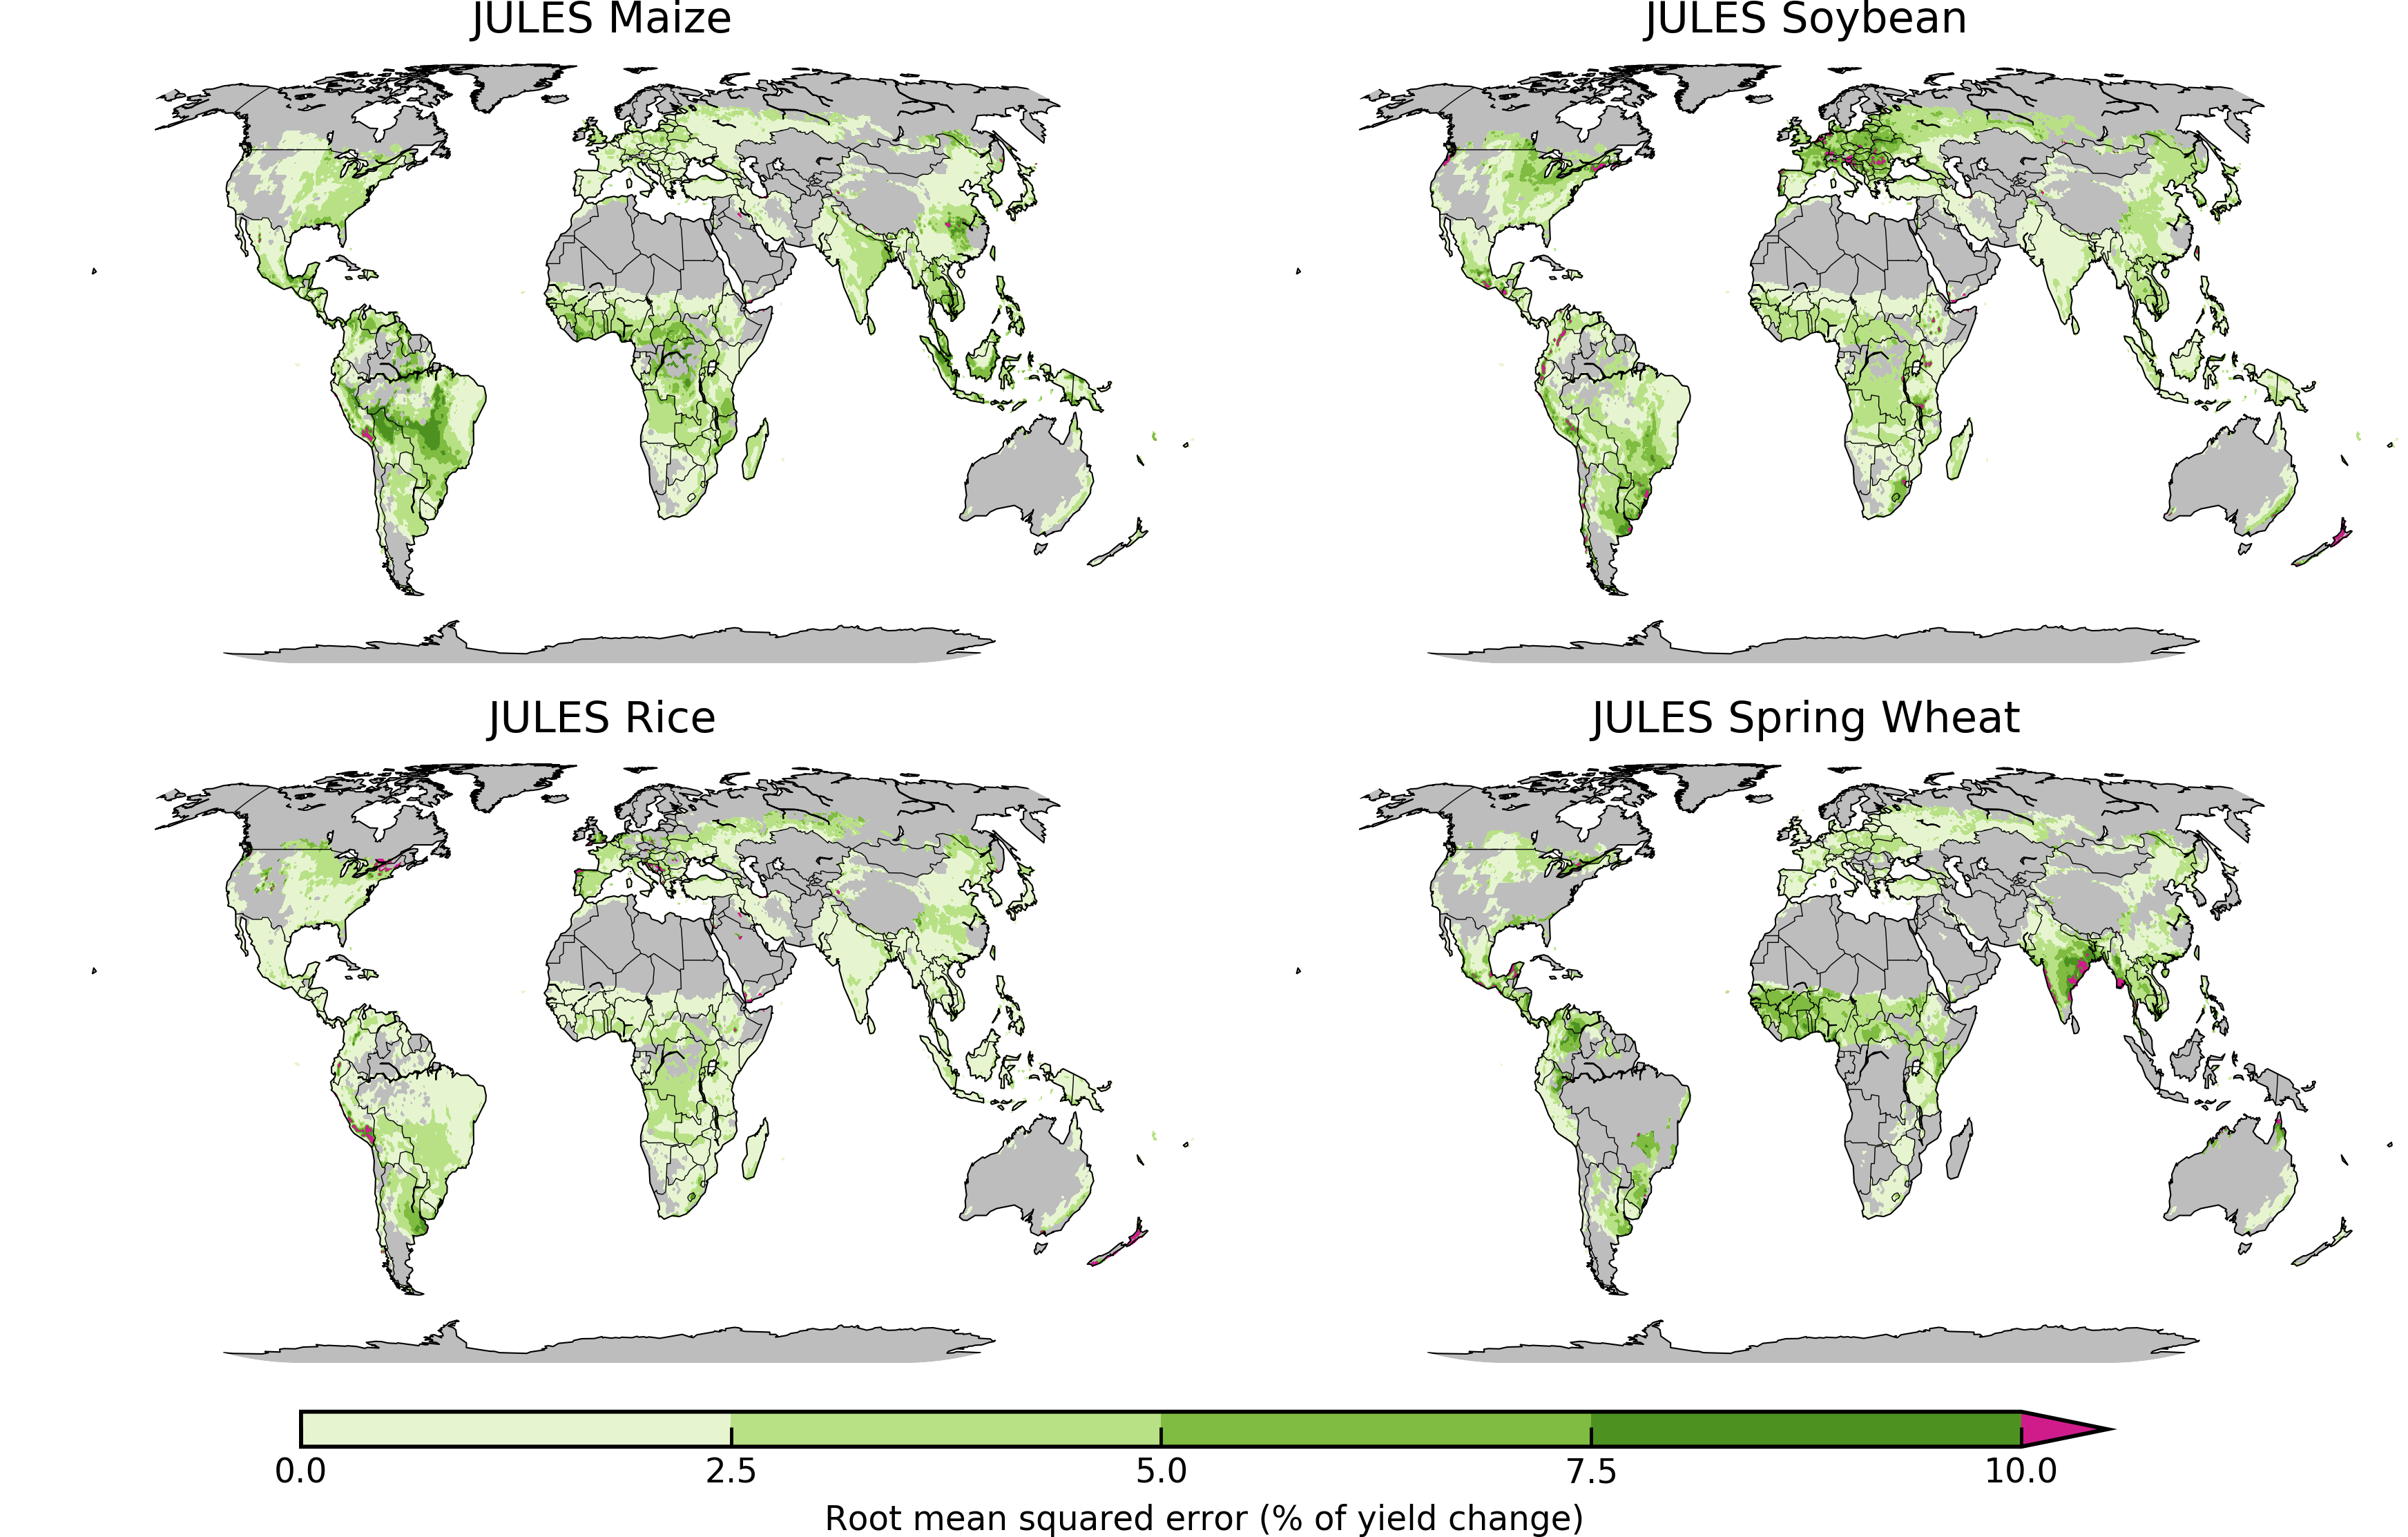
\includegraphics[width=15.5cm]{JULES_spatial_MSE_ton_ha.png}
  \caption{Map of root mean squared error for three fold cross validation process for the JULES model for rainfed crops. Values shown as a percentage of baseline yield in each gridcell.}
\end{figure}

\begin{figure}[h!]
  \centering
  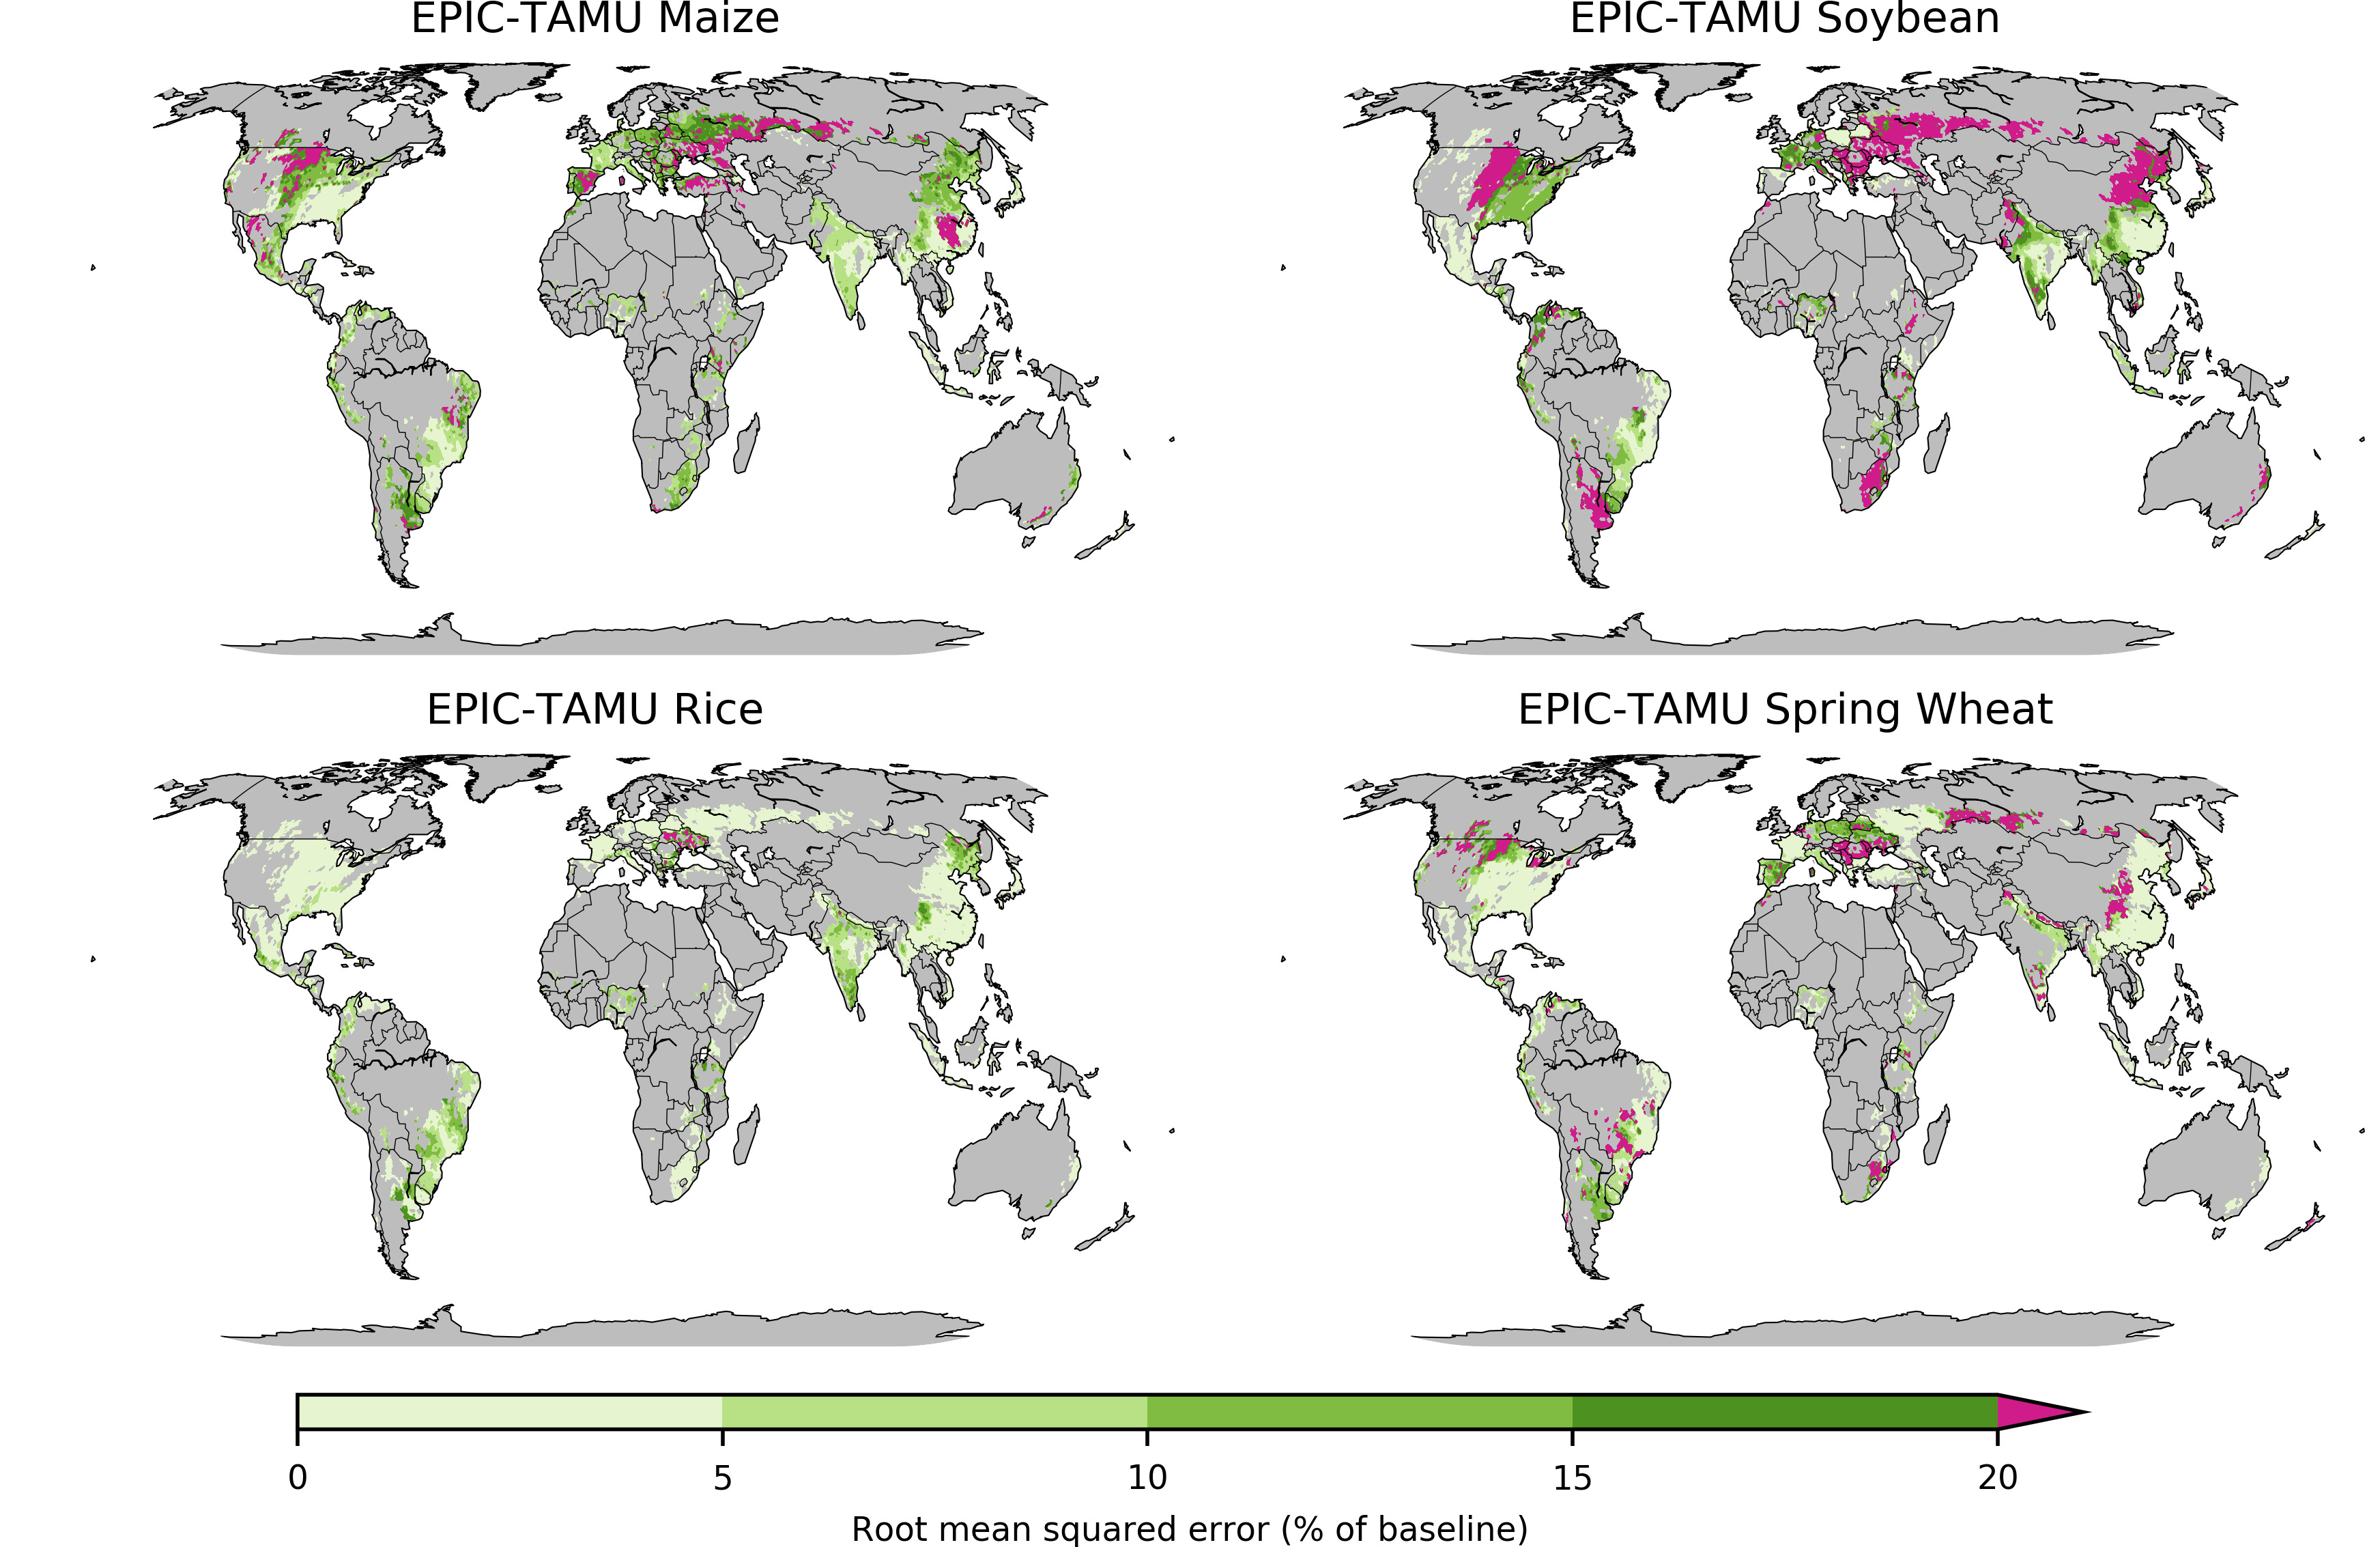
\includegraphics[width=15.5cm]{EPIC-TAMU_spatial_MSE_ton_ha.png}
  \caption{Map of root mean squared error for three fold cross validation process for the EPIC-TAMU model for rainfed crops. Values shown as a percentage of baseline yield in each gridcell.}
\end{figure}

\begin{figure}[h!]
  \centering
  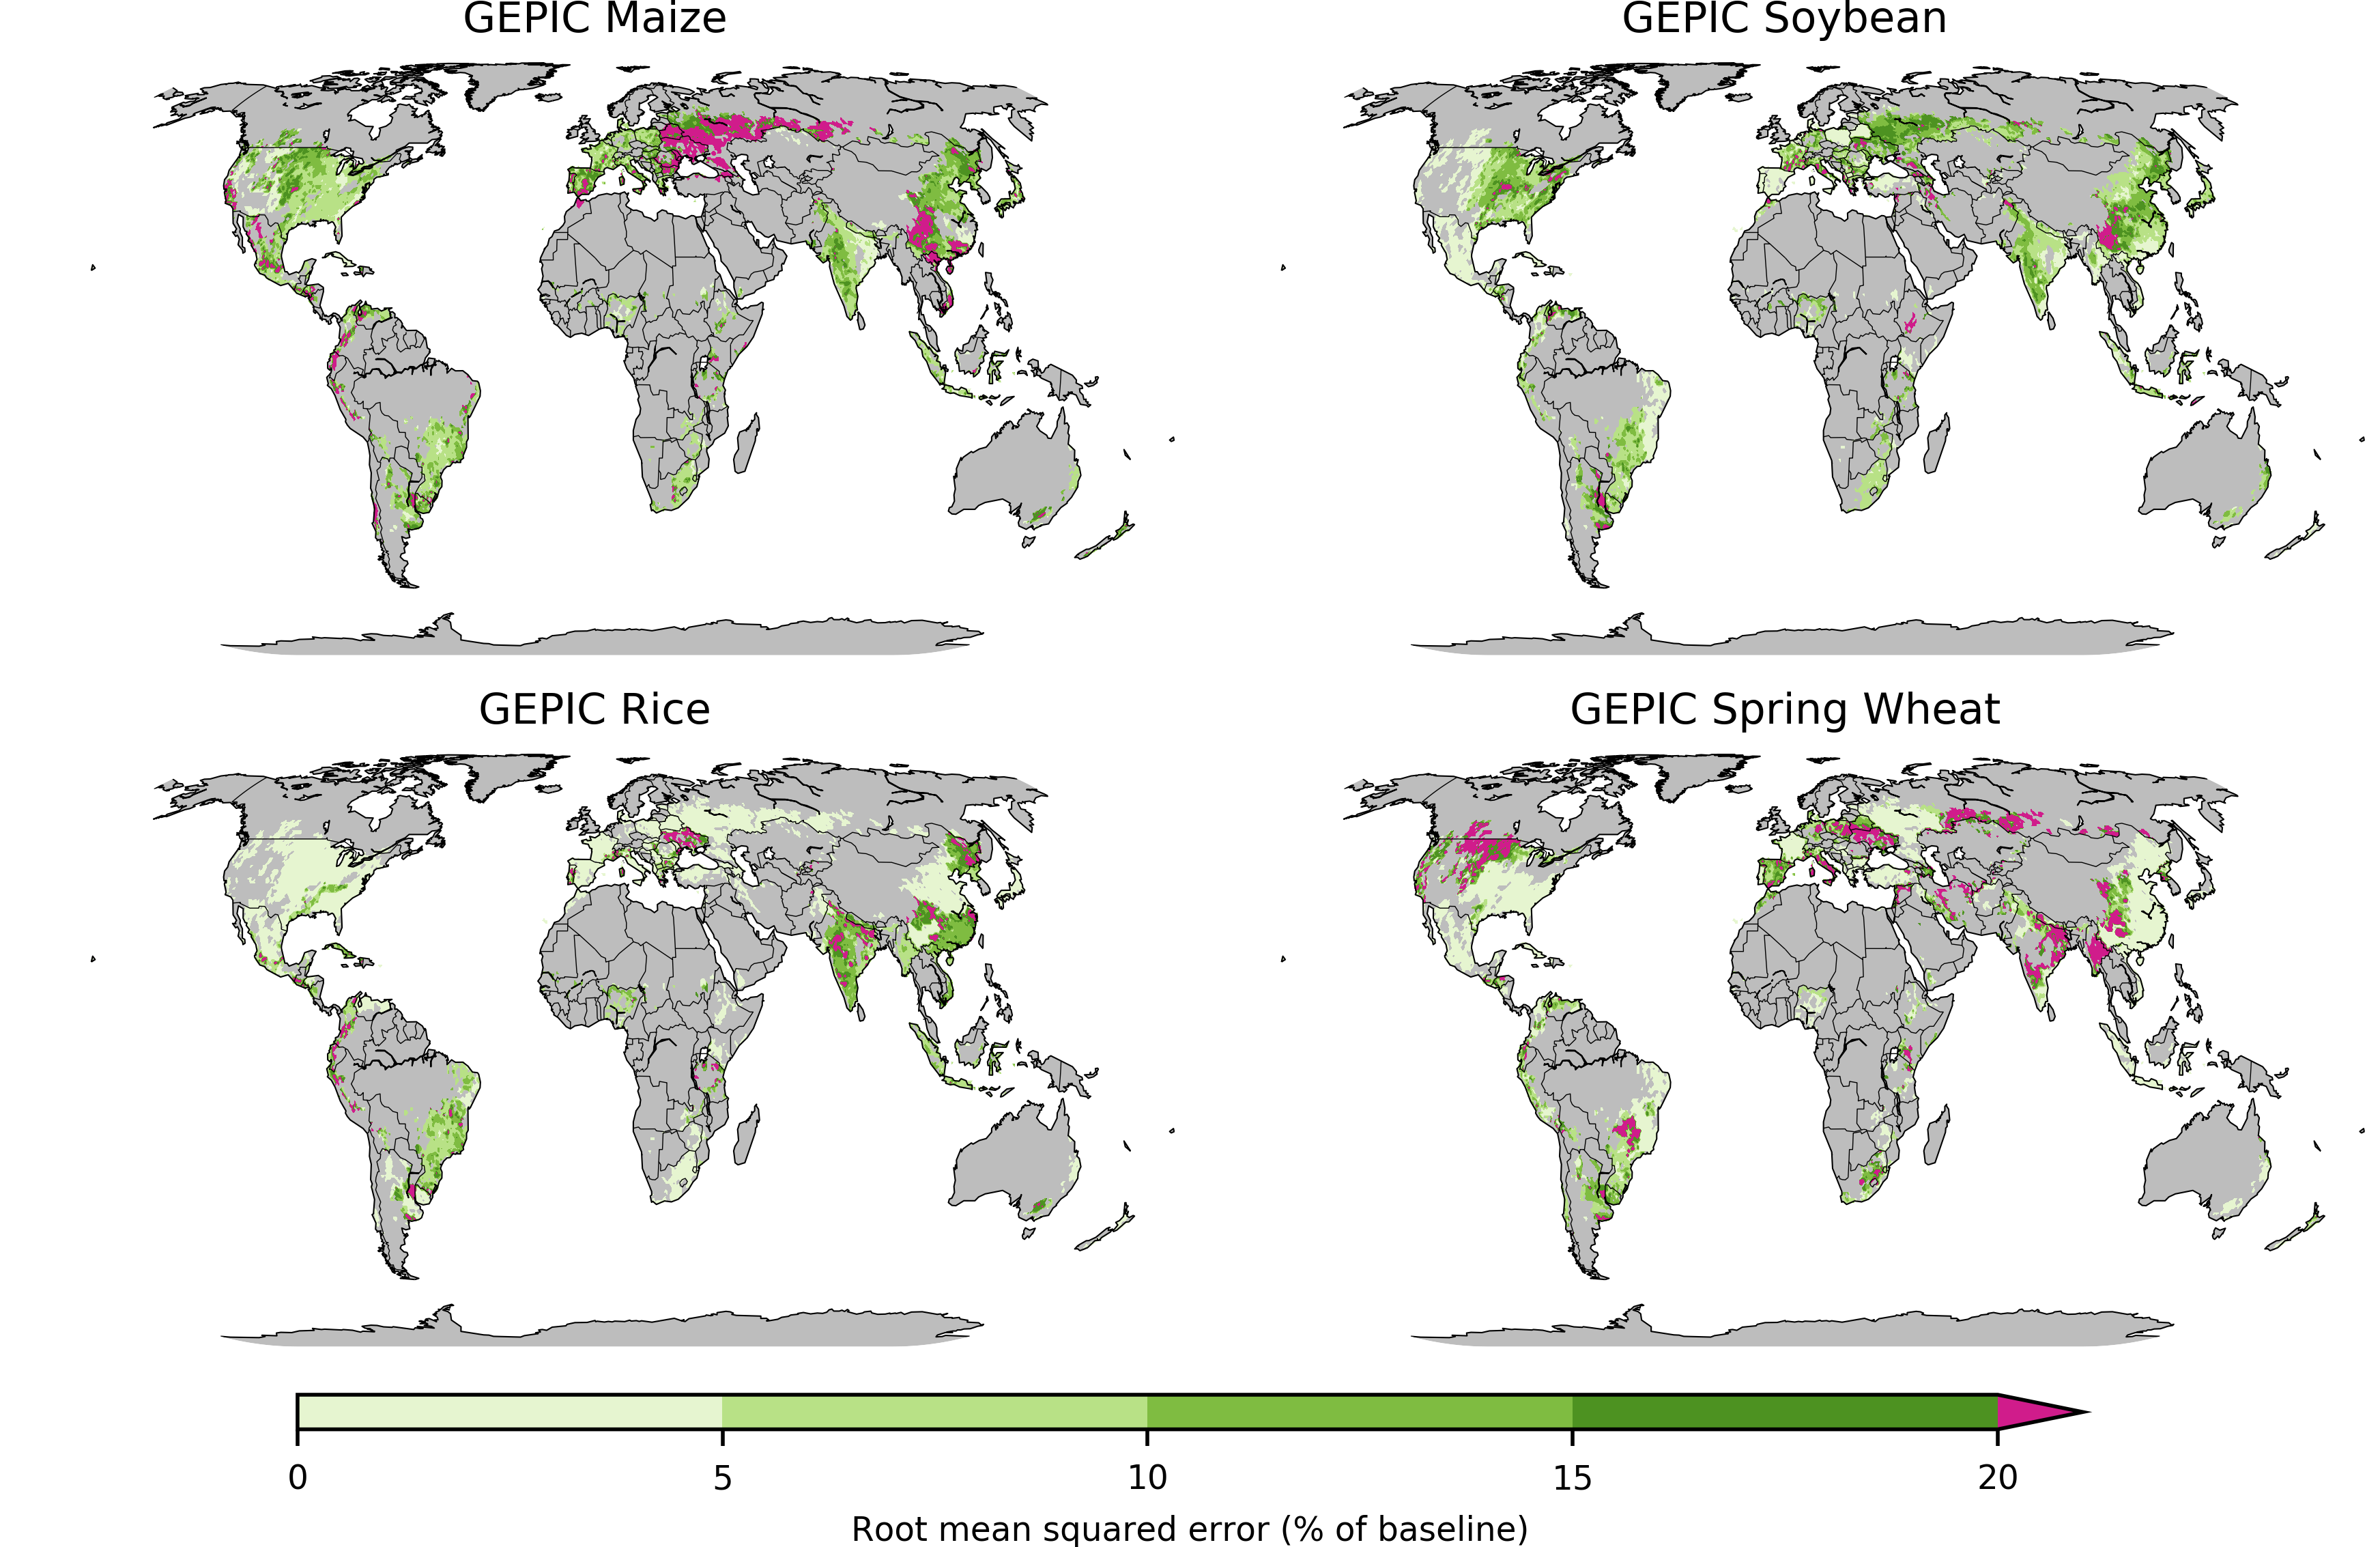
\includegraphics[width=15.5cm]{GEPIC_spatial_MSE_ton_ha.png}
  \caption{Map of root mean squared error for three fold cross validation process for the GEPIC model for rainfed crops. Values shown as a percentage of baseline yield in each gridcell.}
\end{figure}

\begin{figure}[h!]
  \centering
  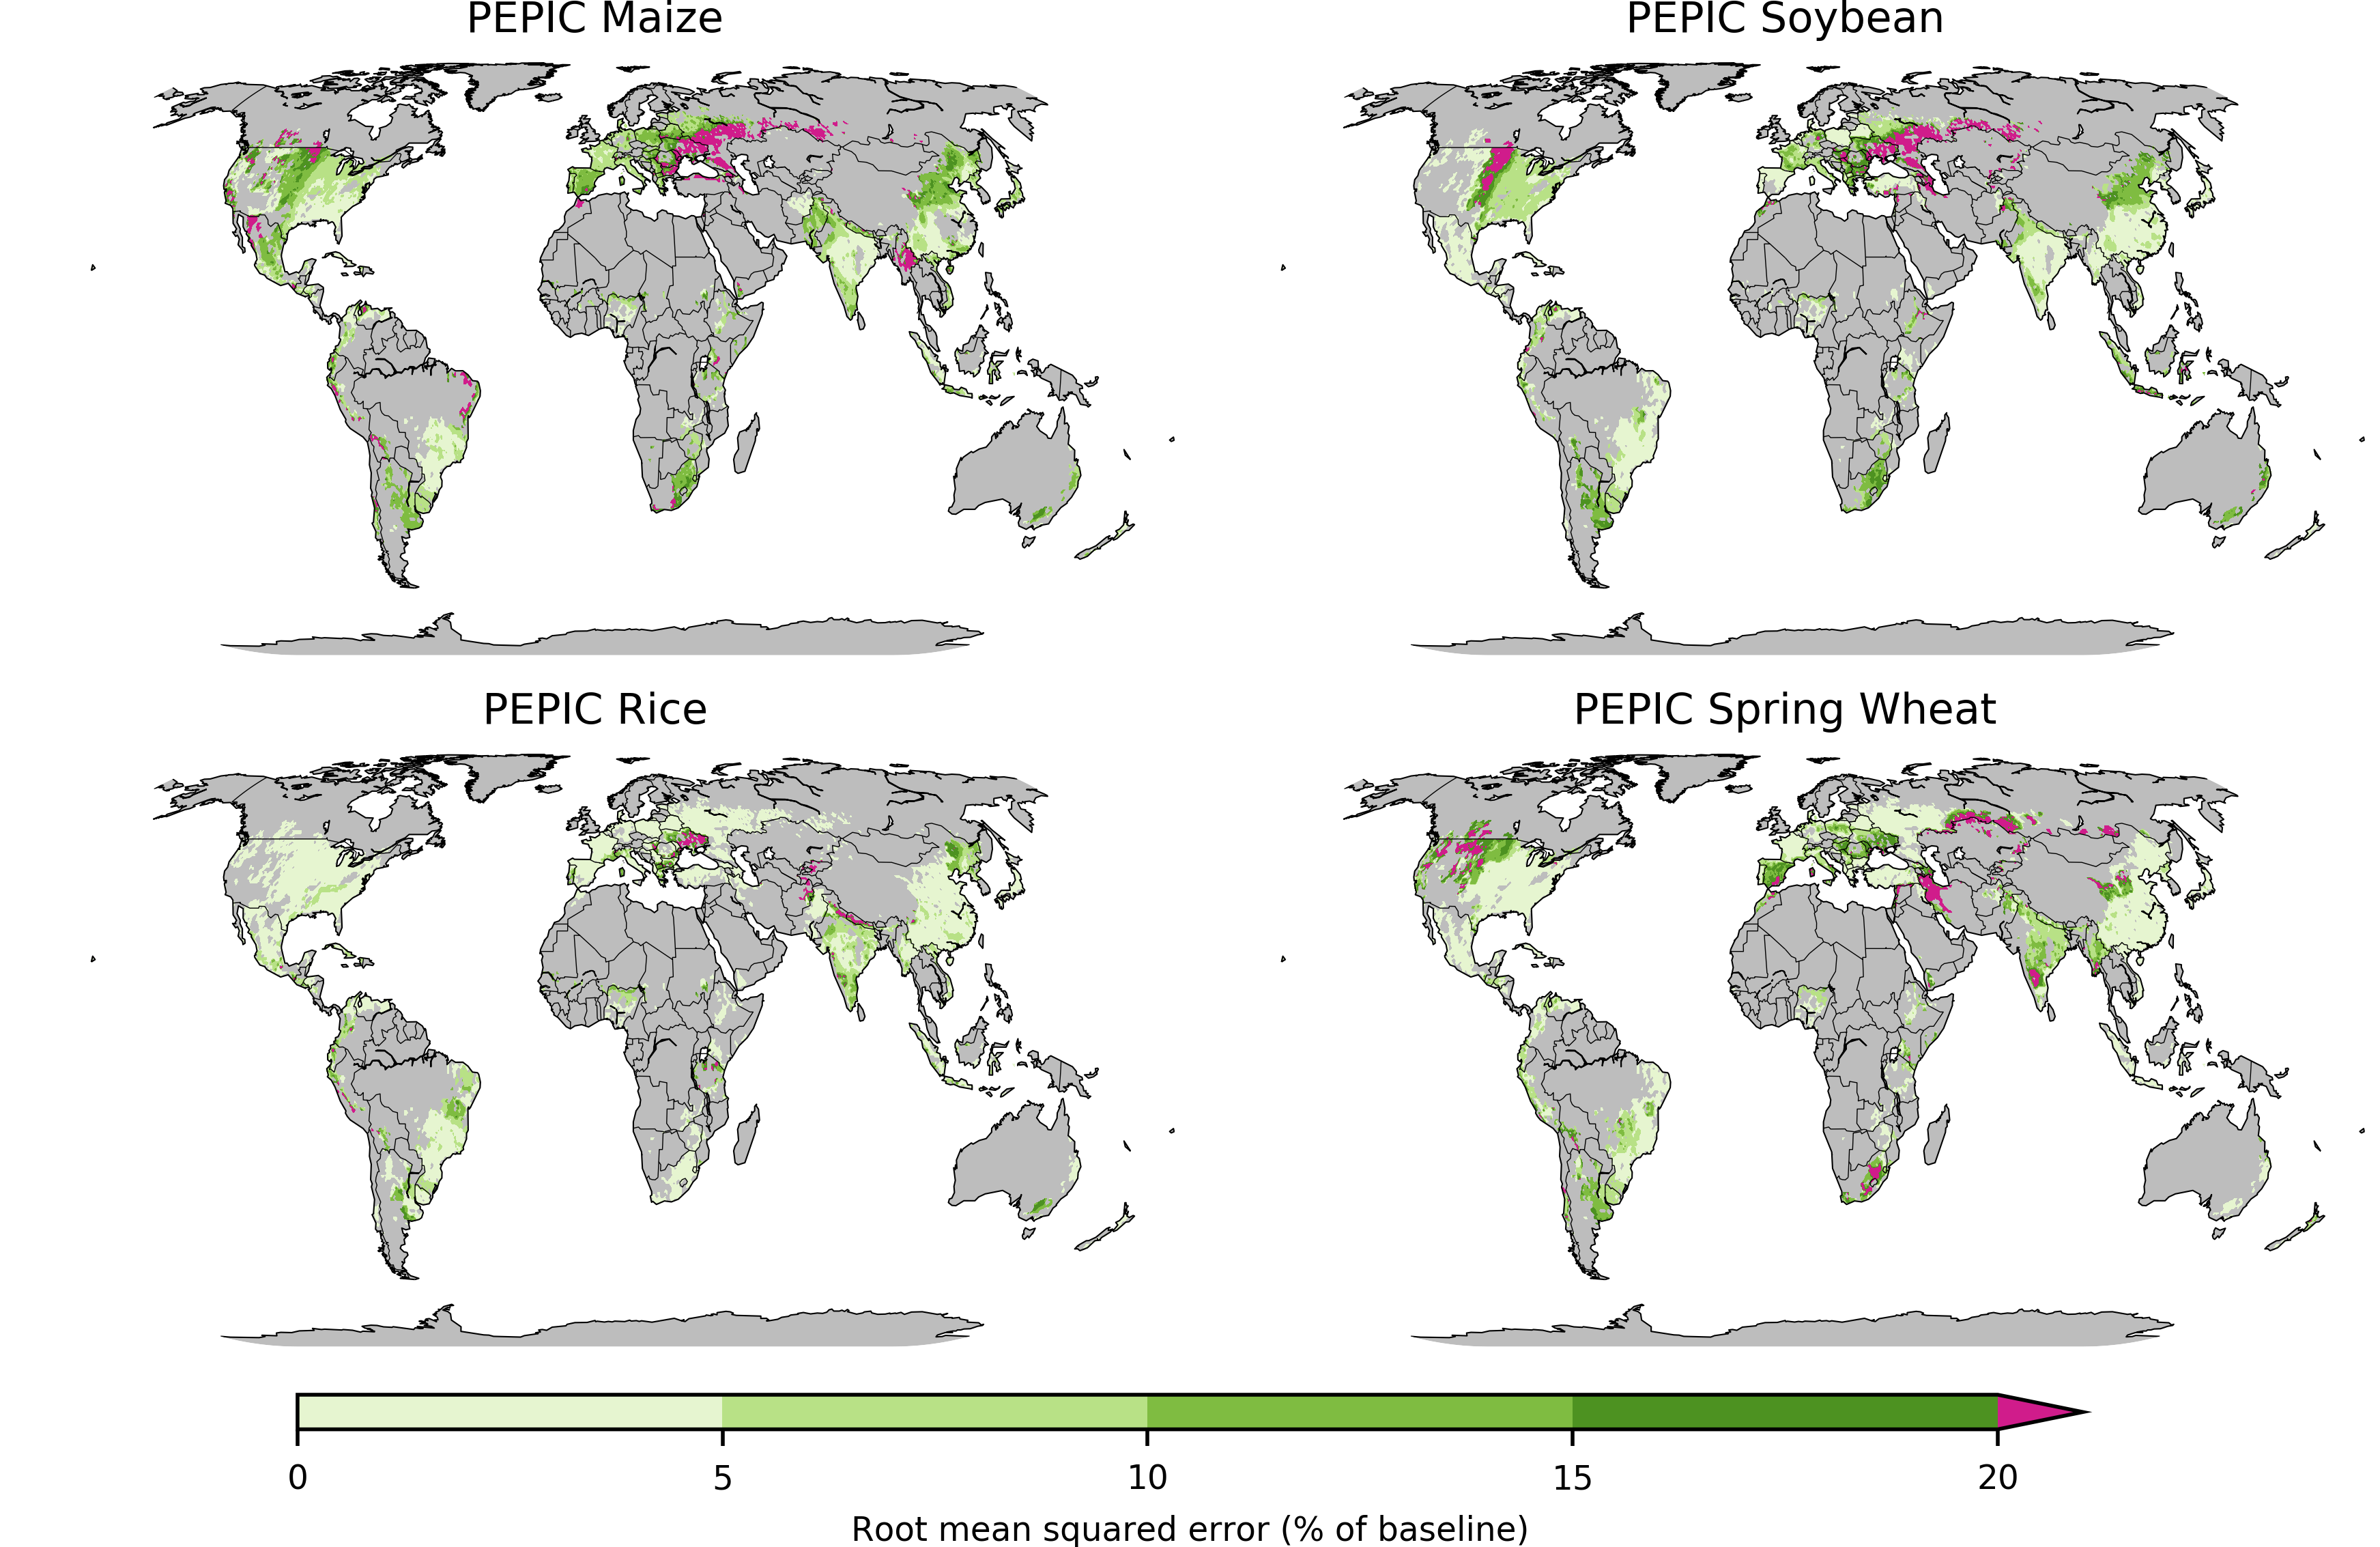
\includegraphics[width=15.5cm]{PEPIC_spatial_MSE_ton_ha.png}
  \caption{Map of root mean squared error for three fold cross validation process for the PEPIC model for rainfed crops. Values shown as a percentage of baseline yield in each gridcell.}
\end{figure}

\end{document}




%%%%%%%%%%%%%%%%%%%%%%%%%%%%%%%%%%%%%%%%%%%%%%%%%%%%%%%%%%%%%%%%%%%%%%%%%%%%%%%%%%%%%%%%%%%%%%%%%%%%%%%%%%%%%%%%
%%%%%%%%%%%%%%%%%%%%%%%%%%%%%%%%%%%%%%%%%%%%%%%%%%%%%%%%%%%%%%%%%%%%%%%%%%%%%%%%%%%%%%%%%%%%%%%%%%%%%%%%%%%%%%%%
%%%%%%%%%%%%%%%%%%%%%%%%%%%%%%%%%%%%%%%%%%%%%%%%%%%%%%%%%%%%%%%%%%%%%%%%%%%%%%%%%%%%%%%%%%%%%%%%%%%%%%%%%%%%%%%%
%%%%%%%%%%%%%%%%%%%%%%%%%%%%%%%%%%%%%%%%%%%%%%%%%%%%%%%%%%%%%%%%%%%%%%%%%%%%%%%%%%%%%%%%%%%%%%%%%%%%%%%%%%%%%%%%
